\documentclass{article}  
\usepackage{graphicx}
\usepackage[utf8]{inputenc}
\usepackage[T1]{fontenc}
\usepackage{float}
\usepackage[italian]{babel}
\usepackage{listings}
\usepackage[usenames]{color}
\usepackage{natbib}
\usepackage{siunitx}
\usepackage[strict]{changepage}
\usepackage{physics}
\usepackage{wrapfig}
\usepackage[a4paper, top=2cm, bottom=2cm, right=2cm, left=2cm]{geometry}
\usepackage{array}
\usepackage{color}
\usepackage{colortbl}
\usepackage{amsmath}
\usepackage{amssymb}
\usepackage{multirow}
\usepackage{enumitem}
\usepackage{hyperref}
\usepackage{times}
\usepackage{booktabs}
\usepackage{subfig}
\usepackage{multirow}



\title{Relazione di laboratorio: studio di catena elettronica}
\author{Docente: dott. Garfagnini, dott. Lunardon \\
Gruppo 14}
\date{Anno accademico 2019/20}

\begin{document}



\maketitle

    \begin{itemize}
        \item[$\circ$] Aidin Attar - 1170698 - aidin.attar@studenti.unipd.it
        \item[$\circ$] Ema Baci - 1171107 – ema.baci@studenti.unipd.it
        \item[$\circ$] Alessandro Bianchetti – 1162147 – alessandro.bianchetti@studenti.unipd.it
    \end{itemize}

\vspace{3 cm}
\begin{large}\textsc{\textbf{Scopo dell'esperienza}: studio della catena elettronica come modello di rivelatore per radiazione ionizzante} 
\end{large}
\vspace{8.5cm}

\begin{figure}[H]
\centering

\includegraphics[scale=0.5, angle=0]{unipd_logo.png}
\end{figure}

%\newpage \tableofcontents \newpage

\twocolumn

\subsection*{Descrizione dell'apparato} La seguente esperienza è stata svolta sul banco di lavoro 1. L'apparato di misura consiste di 
un oscilloscopio digitale Tektronix TBS 1102B EDU, un generatore di funzioni Tektronix AFG 1022, un alimentatore di tensione continua stabilizzato,
due multimetri digitali (Metrix 32292 e Agilent U1230) e una scheda Arduino Due. 
Si è inoltre fatto uso di due integrati TL082C contenenti in tutto 4 amplificatori operazionali.

I circuiti studiati sono stati costruiti sulla basetta millefori alimentando gli amplificatori operazionali come nello schema riportato 
in Figura \ref{fig:alimentazione}

I valori misurati di resistenze e capacità utilizzate verranno riportati in seguito, mentre la procedura per identificare le incertezze
è descritta in appendice.

Infine si è fatto uso di due sonde con fattore di attenuazione 10x precedentemente compensate per la visualizzazione del 
segnale nei due canali dell'oscilloscopio.

Per l'analisi dati sono stati utilizzati programmi scritti in c++, root ed Excel.

\begin{center}
\begin{figure}[ht]
\centering
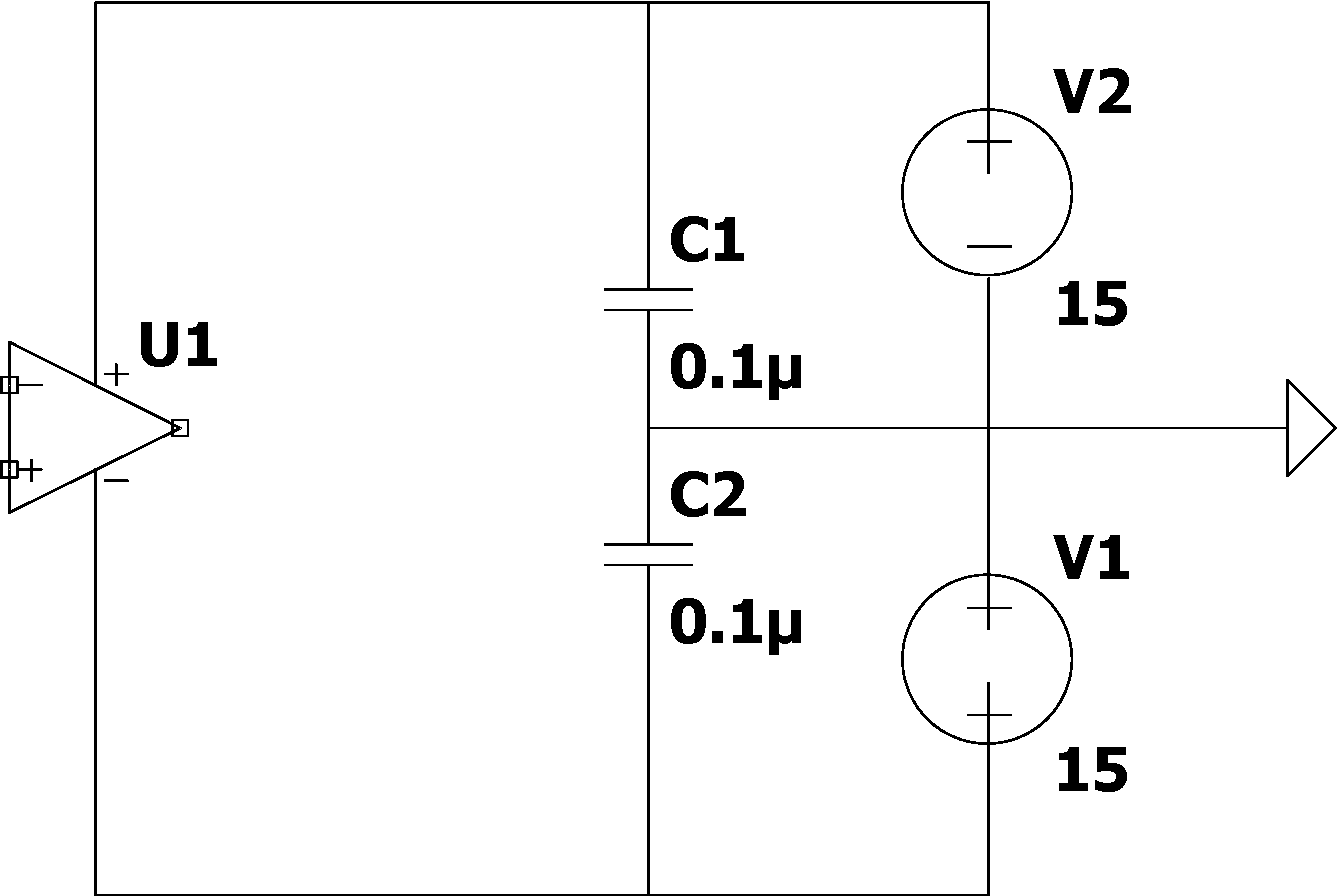
\includegraphics[scale=0.28, angle=0]{alimentazione.pdf}
\caption{ schema per l'alimentazione dell'operazionale }
\label{fig:alimentazione}
\end{figure}
\end{center} 

\section{Preamplificatore di carica}

\subsection{Breve discussione del circuito}

Lo scopo dell'esperienza completa è costruire un circuito che possa rilevare piccoli segnali, amplificarli tanto da poterli processare con più facilità
e poi amplificarli ulteriormente per offrirli allo sperimentatore. Il primo passo della realizzazione di tale \textit{catena elettronica} è il circuito
preamplificatore. Qui il generatore di funzioni è utilizzato proprio per simulare piccoli segnali di cui sopra analoghi a quelli che proverrebbero tipicamente 
da esperienze di spettrocopia: si forniscono dunque in ingresso impulsi di tensione (PULSE) come quelli che produrrebbe il passaggio di una radiazione ionizzante in 
un volume di gas. 
Si è dunque costruito il circuito come in Figura \ref{fig:preamp}
\begin{center}
\begin{figure}[ht]
\centering
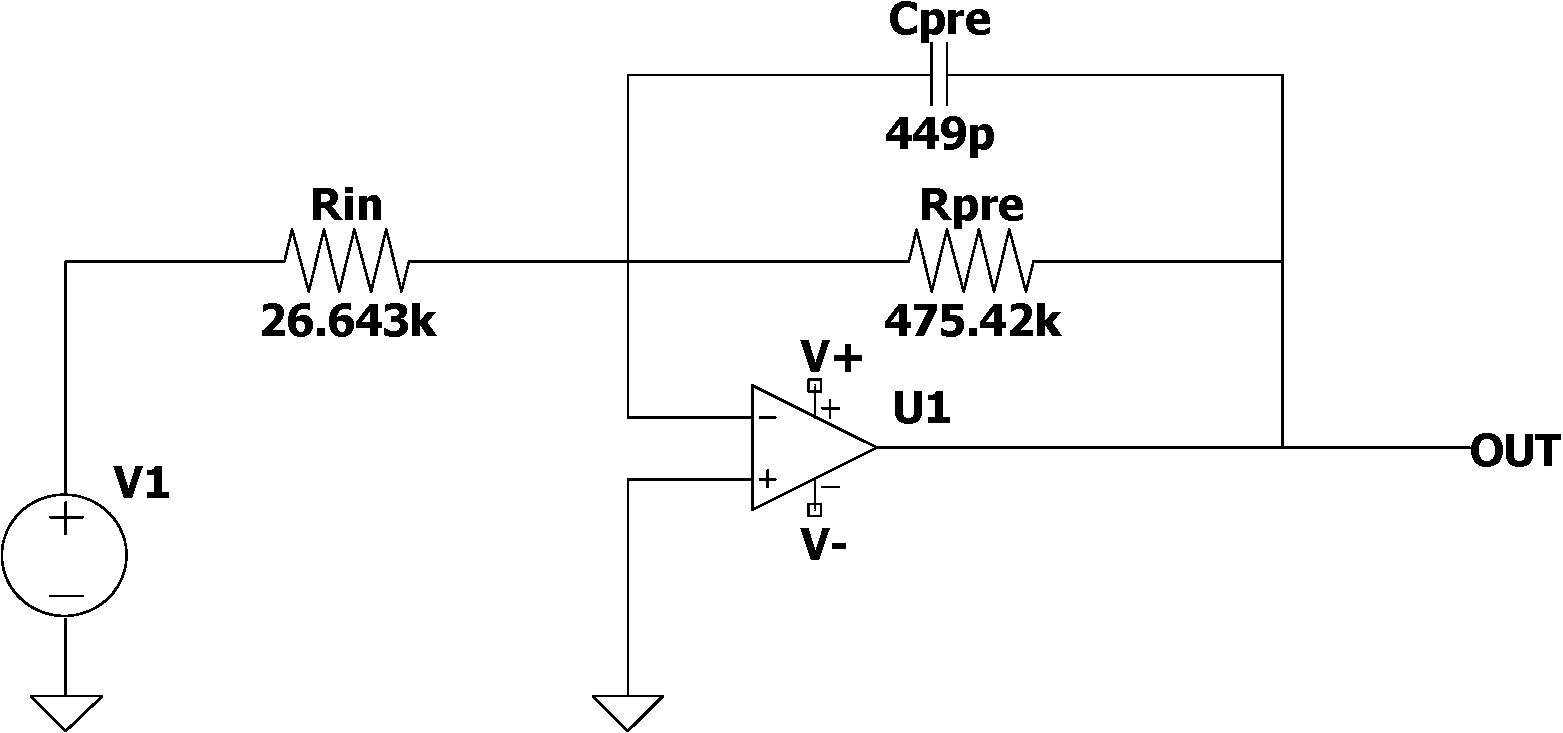
\includegraphics[scale=0.3, angle=0]{preamp.pdf}
\caption{ circuito amplificatore di carica }
\label{fig:preamp}
\end{figure}
\end{center}
La funzione di trasferimento è data, nel formalismo di Laplace, da
\begin{equation}
    \label{eqn:preamp_Laplace}
    H(s) = -\frac{R_{pre}}{R_{in}} \frac{1}{1+sR_{pre}C_{pre}}
\end{equation}
in cui possiamo effettuare la sostituzione $s \longleftrightarrow i\omega$ per riprodurre la soluzione stazionaria. Considerando poi
solamente il modulo, e definendo il tempo caratteristico $\tau_{pre}=R_{pre}C_{pre}$, avremo
\begin{equation}
    \label{eqn:preamp_trasf}
    H(\omega) = \frac{R_{pre}}{R_{in}} \frac{1}{\sqrt{1+\omega^2\tau_{pre}^2}}
\end{equation}

Si osserva inoltre che inserendo nella formula \ref{eqn:preamp_Laplace} la trasformata di Laplace dell'impulso di tensione, pari a 
$V_{in}$/s, si otterrà in uscita, antitrasformando opportunamente, un segnale esponenziale corrispondente a

\begin{equation}
    \label{eqn:Vout1_preamp}
    V_{pre}^{pulse}(t) = -\frac{R_{pre}}{R_{in}}V_{in}(1-e^{-\frac{t}{\tau_{pre}}})
\end{equation}

Quest'ultima è valida finché dura l'impulso di tensione: essendo $T_{pulse} << \tau_{pre}$, potremo considerare l'espansione in 
serie di Taylor della \ref{eqn:Vout1_preamp}, ottenendo una discesa lineare. Tale discesa lineare si interromperà all'esaurirsi dell'
impulso in ingresso, lasciando posto alla formula della scarica del condensatore $C_{pre}$, caricato proprio dallo stesso impulso.
Ne risulta un grafico che ha un picco negativo $V_{pre}^{max}$ in corrispondenza di t = $T_{pulse}$, per poi risalire con la curva esponenziale
dettata da

\begin{equation}
    \label{eqn:Vout2_preamp}
    V_{pre}^{RC}(t) = V_{pre}^{max}e^{-\frac{t}{\tau_{pre}}}.
\end{equation}

\subsection{Discussione dati}

Si precisa che sono stati suggeriti dei valori per i parametri del circuito $\tau_{pre,th} = 220 \mu$s e $C_{pre} = 450$ pF, con $R_{pre}$ calcolato di 
conseguenza. Pertanto i valori misurati con il multimetro Metrix 32292 sono
\begin{align*}
    R_{pre} = (475.4 \pm 0.2)\text{k}\Omega \quad \sigma_{\%}=0.04 \% \\    
    C_{pre} = (149 \pm 14) \text{pF} \quad \sigma_{\%}=3.1 \%    \\
    \tau_{pre,th} = (213 \pm 7)\mu \text{s} \quad \sigma_{\%}=3.1 \%     \\
\end{align*}
Si è dunque impostato un impulso della durata di $T_{pulse}$ = $2 \mu$s: sapendo inoltre che la carica da iniettare 
corrispondeva a $Q_{in}^{th}$ = 80 pC e che la resistenza di ingresso scelta misurava $R_{in}=(26.64\pm0.01)$ k$\Omega$ ($\sigma_{\%}=0.04\%$), 
si è selezionata l'altezza $V_{in}$ dell'impulso in modo che fosse soddisfatta la relazione
\begin{equation}
    \label{eqn:Qin}
    Q_{in} = \frac{V_{in}}{R_{in}} T_{pulse}.
\end{equation}
Ne si è ricavato $V_{in}^{th} =1.06 $V. Per controllare la correttezza del circuito si è misurato il picco $V_{pre}^{max}$,
dato, utilizzando l'approssimazione della \ref{eqn:Vout1_preamp}, da
\begin{equation}
    \label{eqn:Vpre_max}
    V_{pre}^{max} = -\frac{R_{pre}}{R_{in}} V_{in} \frac{T_{pulse}}{\tau_{pre}} = - \frac{Q_{in}}{C_{pre}}
\end{equation}
da cui, inserendo il valore misurato $V_{in}^{th}=(1.02\pm 0.02) $V, si ricava $V_{pre,th}^{max} =  (-170 \pm 6) $mV. Invece dalla 
misura si ottiene $V_{pre,sper}^{max} = (-176 \pm 4) $mV, per cui $\lambda = 0.76$ e lo scostamento percentuale è $\epsilon = 3.2 \%$, 
ossia il valore misurato è ottimamente compatibile con quello atteso.

Si è inoltre la verificata la linearità tra $Q_{in}$ e $V_{pre}^{max}$ descritta da \ref{eqn:Vpre_max} variando la durata dell'impulso
in ingresso e quindi la carica iniettata nel circuito secondo \ref{eqn:Qin}. Si riportano quindi in grafico i punti, la retta 
interpolante e i principali parametri di bontà del fit. 

\begin{center}
\begin{figure}[H]
\centering
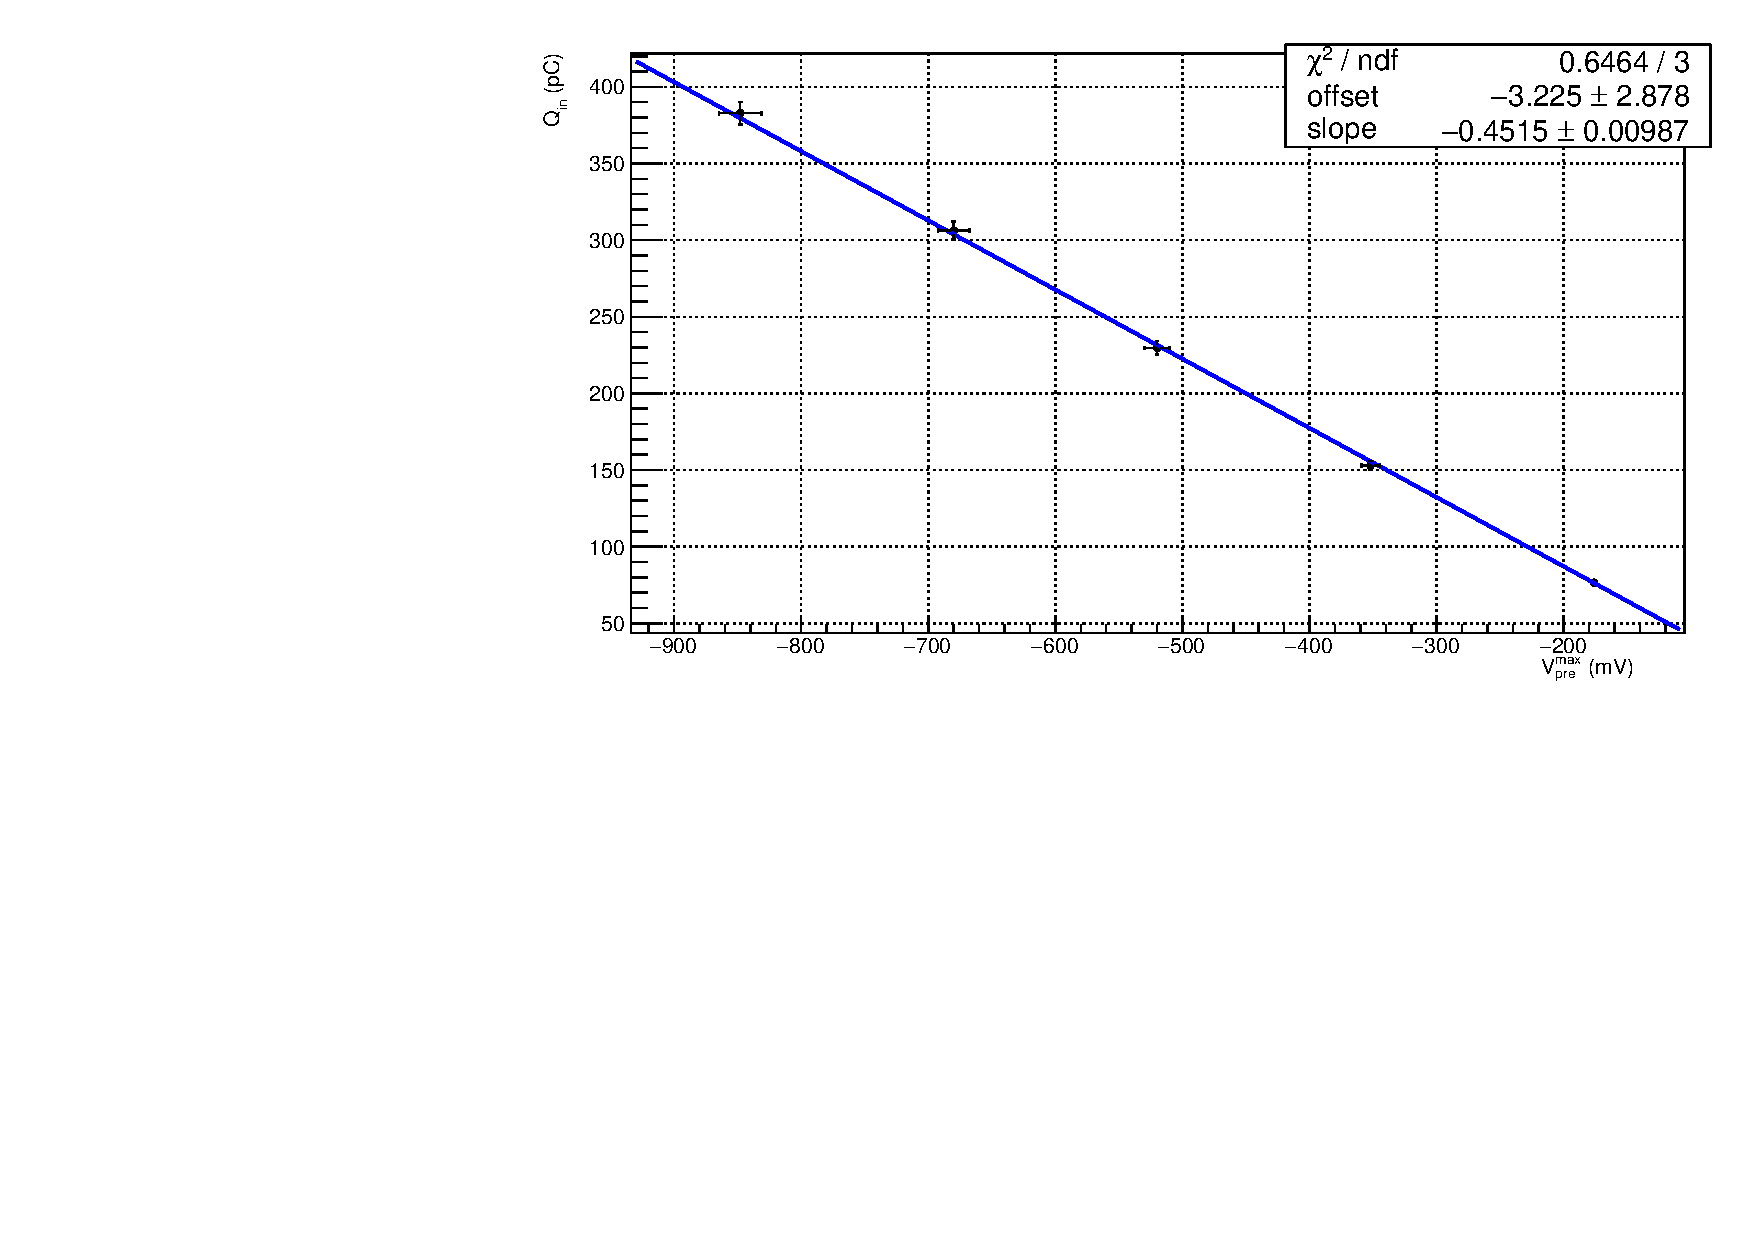
\includegraphics[scale=0.4, angle=0]{fitpreamp.pdf}
\setlength{\belowcaptionskip}{-20pt}
\caption{carica iniettata e picco di tensione in uscita}
\label{fig:QinvsVpre}
\end{figure}
\end{center}

\begin{center}
    \begin{figure}[H]
        \centering
        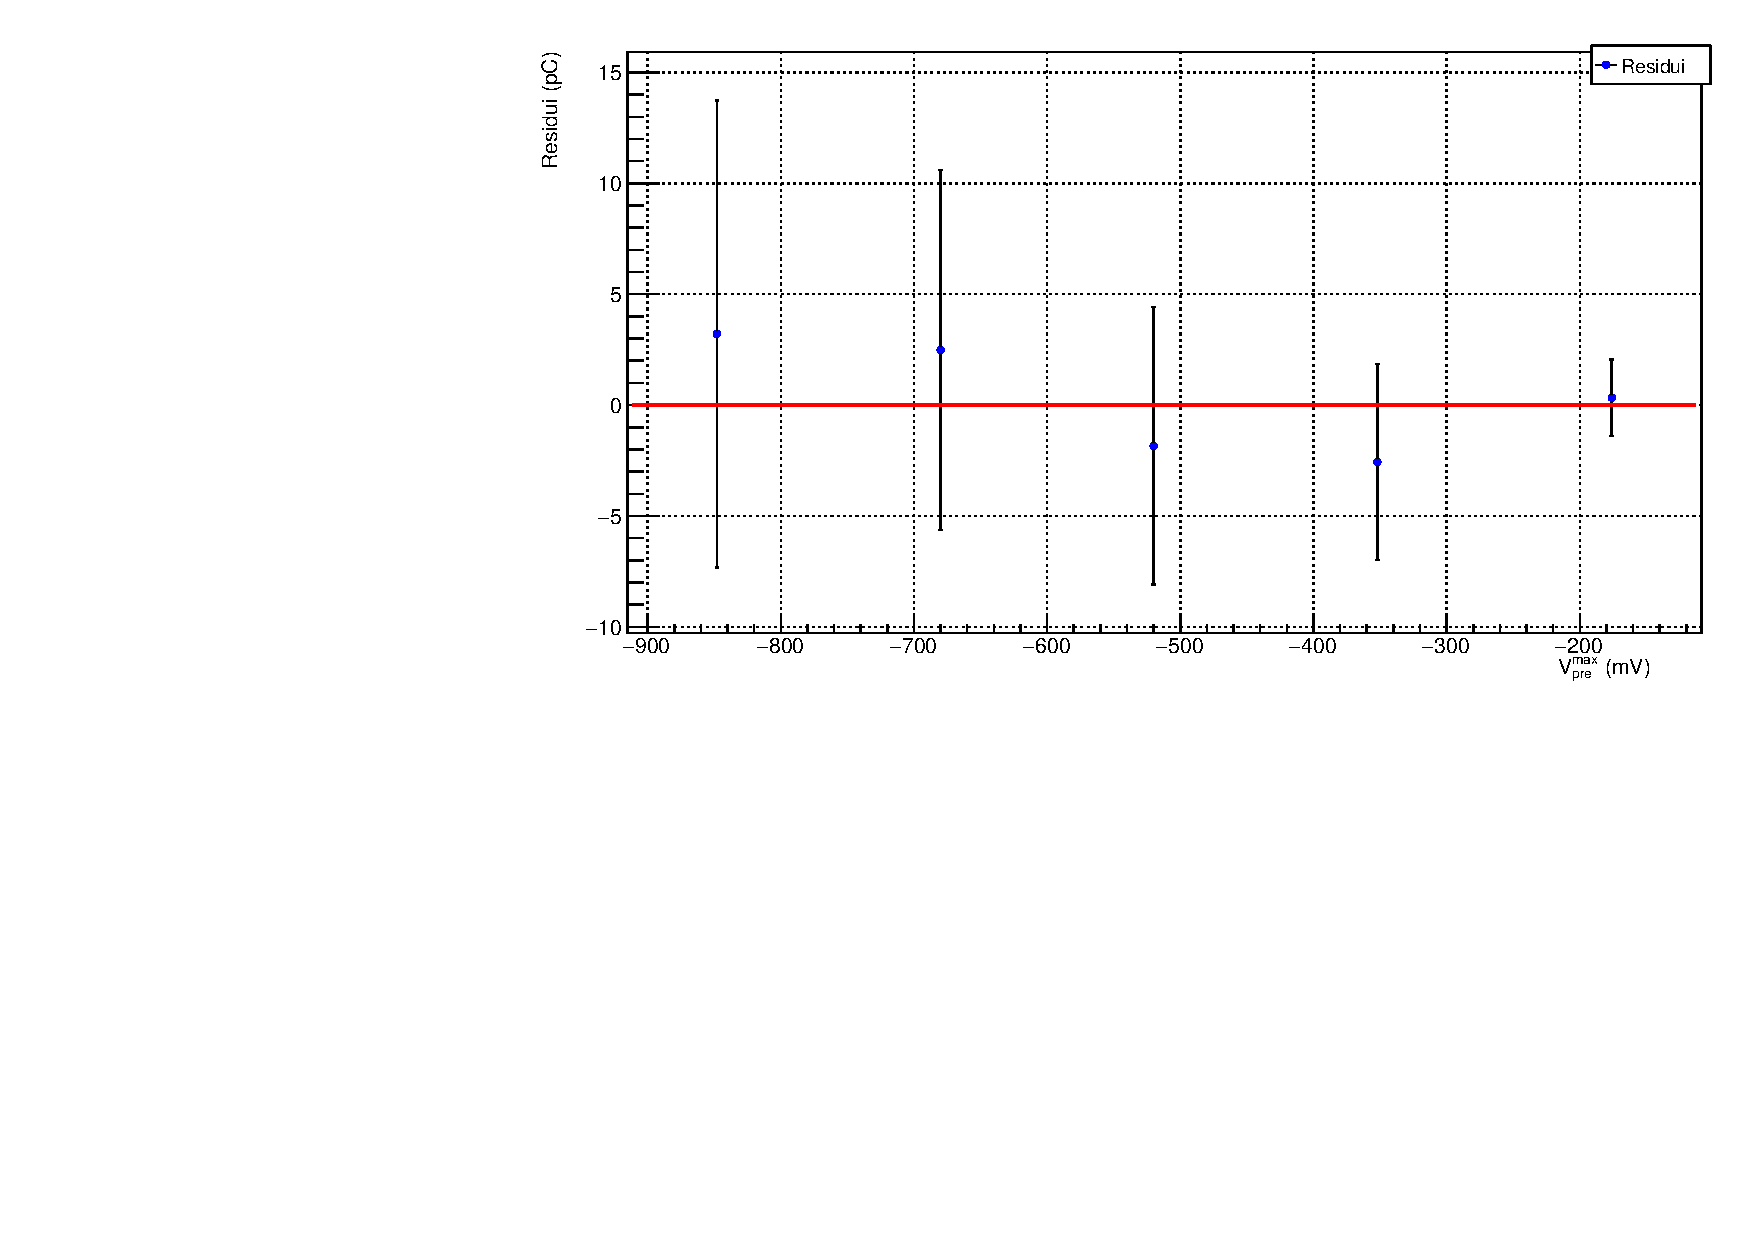
\includegraphics[scale=0.4, angle=0]{residuipreamp.pdf}
        \setlength{\belowcaptionskip}{-20pt}
        \caption{grafico dei residui della relazione tra $Q_{in}$ e $V_{pre}^{max}$}
        \label{fig:QinvsVpre_res}
    \end{figure}
\end{center}

\begin{table}[ht]
    \centering
    \begin{tabular}{ccccc}
        \toprule
        $\sigma_{y, post}$    &$\chi^{(2)}$    &$\lambda_{\chi}$   &$\rho$ &t      \\
        \midrule
        3.0 pC                  &0.65            &0.96               &-0.9998&-109.14\\
        \bottomrule
    \end{tabular}
    \caption{parametri di verifica della bontà del fit}
\end{table}

Si specifica che il fit è stato effettuato utilizzando
gli errori di entrambe le coordinate, poichè nessuno dei 
due errori relativi è risultato trascurabile rispetto all'altro.
Gli estimatori danno tutti risposta positiva, quindi possiamo concludere che la relazione lineare è ben verificata.
Inoltre dal valore di pendenza, considerando la legge lineare \ref{eqn:Vpre_max}, è possibile ottenere una stima sperimentale della capacità $C_{pre}$, 
da confrontare con il valore misurato. Si ricava quindi $C_{pre,sper} = (452\pm 10)$pF, che ha $\lambda = 0.15 $ rispetto al valore misurato.

Inoltre dallo studio della \ref{eqn:Vout2_preamp}, e in particolare della sua linearizzazione logaritmica, è possibile ricavare
una stima sperimentale di $\tau_{pre}$. Infatti applicando il logaritmo naturale si ottiene
\begin{equation}
    \log V(t) = \log V_{pre}^{max} - \frac{t}{\tau_{pre}}
\end{equation}
per cui si trova una relazione lineare tra $\log V(t)$ e t, da cui $\tau_{pre}$=-1/b con b slope del fit.
Si riporta il grafico di tempi e logaritmi delle tensioni, interpolati linearmente, e il relativo grafico dei residui

\begin{center}
\begin{figure}[H]
\centering
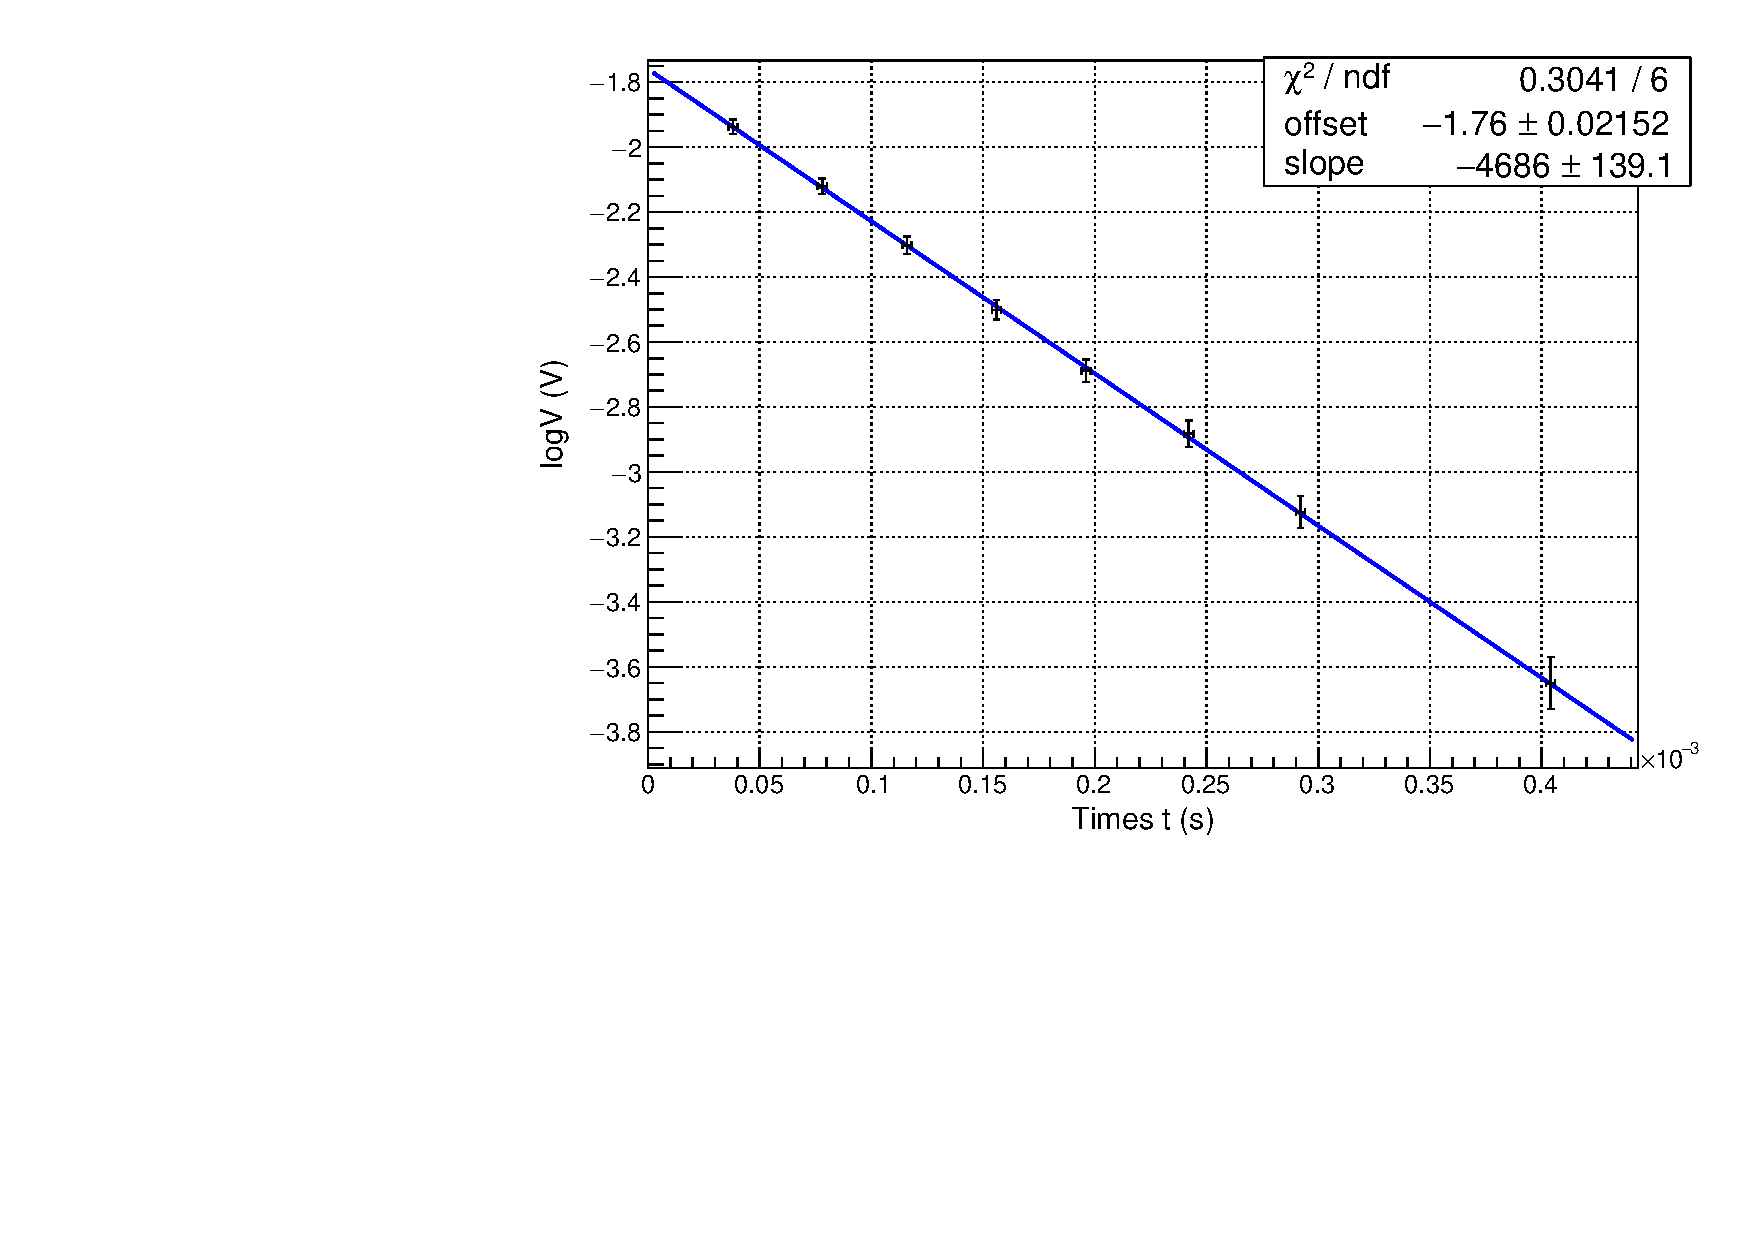
\includegraphics[scale=0.4, angle=0]{preampRC.pdf}
\setlength{\belowcaptionskip}{-20pt}
\caption{relazione lineare tra logaritmi delle tensioni e tempi}
\label{fig:QinvsVsh}
\end{figure}
\end{center}

\begin{center}
\begin{figure}[H]
\centering
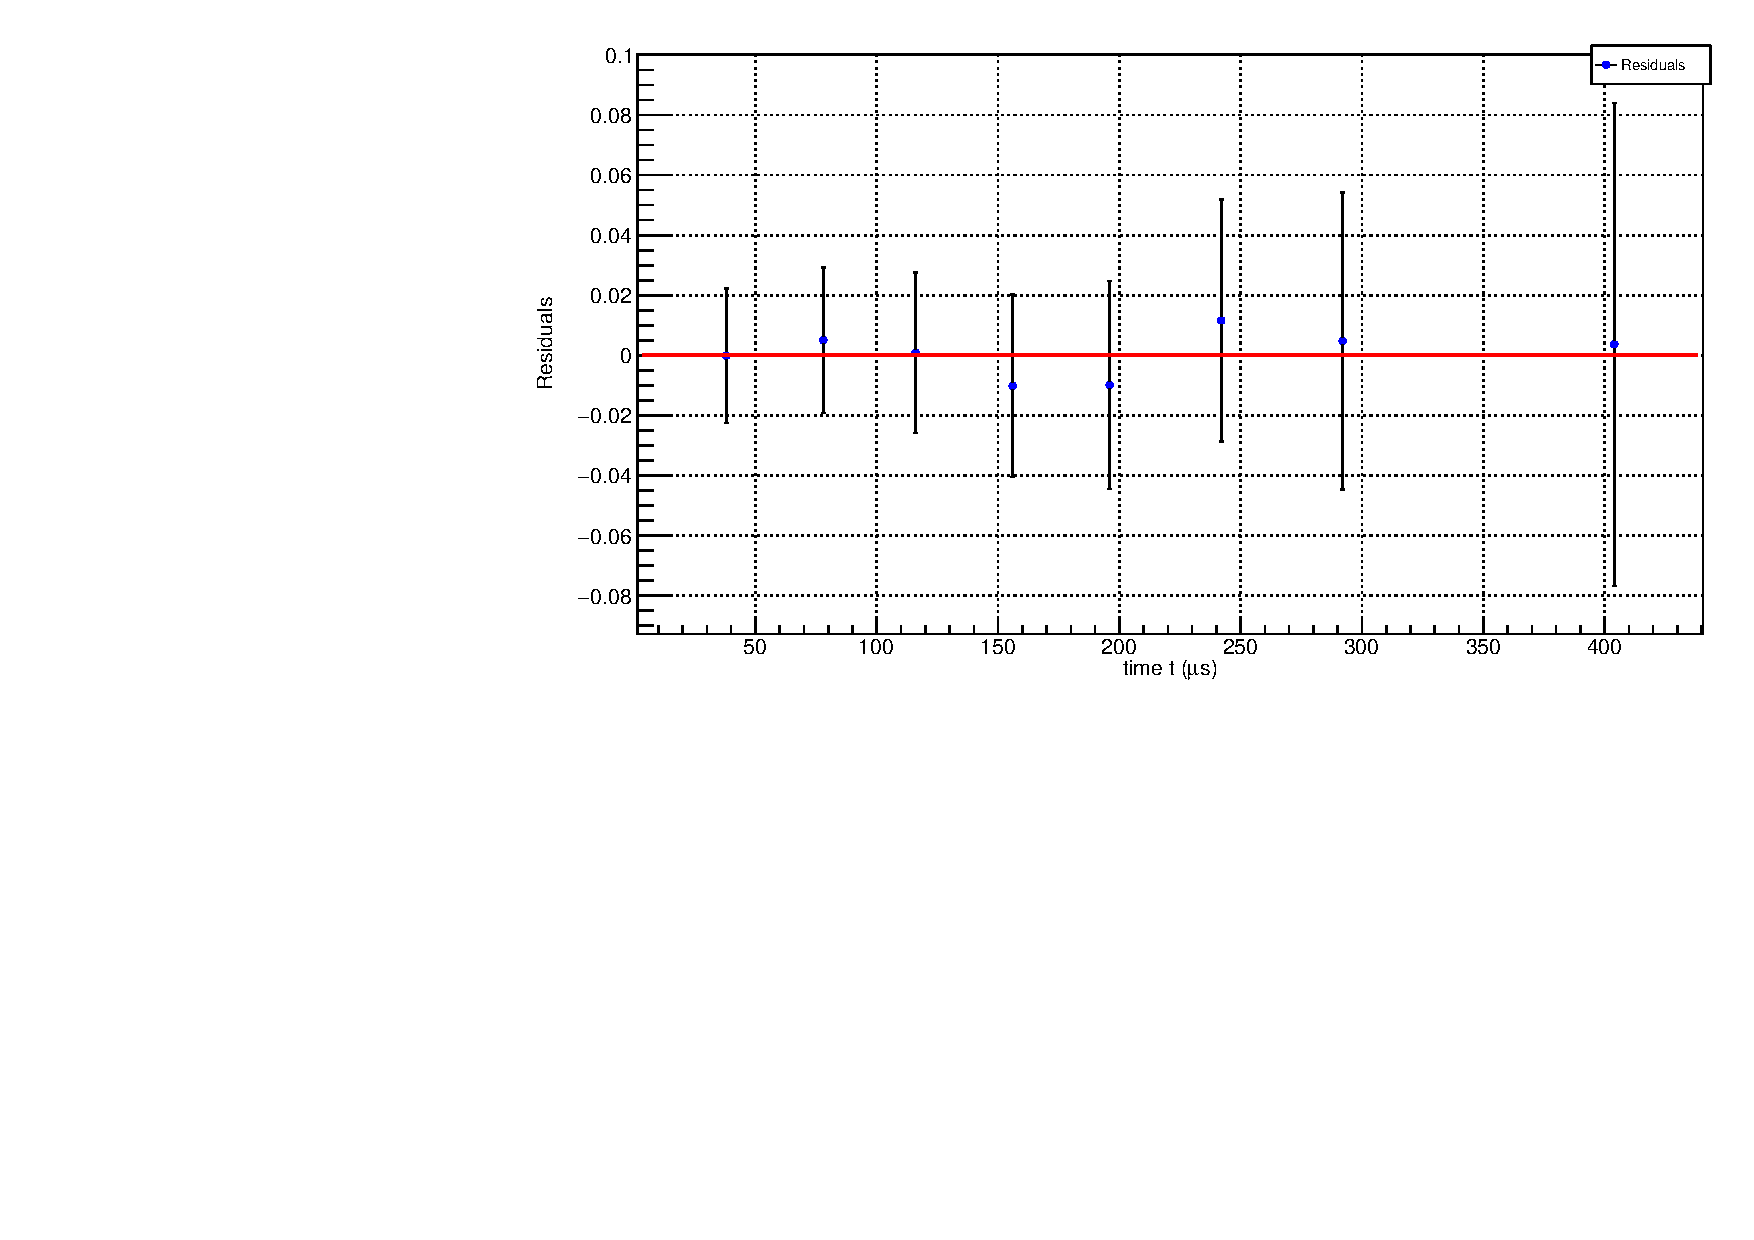
\includegraphics[scale=0.4, angle=0]{preampRCresidui.pdf}
\setlength{\belowcaptionskip}{-20pt}
\caption{grafico dei residui della relazione tra $\log V$ e t}
\label{fig:QinvsVshRESIDUI}
\end{figure}
\end{center}

\begin{table}[ht]
    \centering
    \begin{tabular}{ccccc}
        \toprule
        $\sigma_{y, post}$    &$\chi^{(2)}$    &$\lambda_{\chi}$   &$\rho$  &t   \\
        \midrule
        0.008 V               &0.33            &1.64              &-0.99991&-189.59\\
        \bottomrule
    \end{tabular}
    \caption{parametri di verifica della bontà del fit}
\end{table}

Si osserva la buona riuscita del fit, che verifica la scarica RC del circuito al termine dell'impulso.
Tuttavia è possibile notare una forte sovrastima degli errori sia visivamente osservando il grafico dei
residui in Figura \ref{fig:QinvsVshRESIDUI}, sia osservando il valore molto basso di $\chi^{(2)}$

Dal valore della pendenza, come anticipato prima, ricaviamo una stima di $\tau_{pre}^{sper}$. A scopo di controllo, è inoltre possibile 
ottenere una valutazione di $V_{pre}^{max}$ usando il parametro di offset a sapendo $V_{pre}^{max} = e^a$. Si riportano quindi i due
valori calcolati con i loro errori calcolati per propagazione.

\[\tau_{pre}^{sper} = (213 \pm 6)\mu \text{s} \quad \sigma_{\%} = 2.9 \%    \]
\[V_{pre}^{max} = (-172 \pm 3)\text{mV} \quad \sigma_{\%} = 2.0 \%\]
che risultano ottimamente compatibili con i valori attesi  $\tau_{pre}^{th}$ e $V_{pre,th}^{max}$, in quanto $\lambda_{\tau} = 0.01$
e $\lambda_{V}=0.2$.
 
\medskip

Si è infine effettuato uno studio in frequenza del circuito con lo scopo di verificare la \ref{eqn:preamp_trasf}, variando la frequenza
e verificando il variare del modulo dell'amplificazione di fronte a un ingresso sinusoidale.
Si riporta in particolare il grafico di Bode che raffigura frequenza e amplificazione in dB: ai punti sperimentali si è affiancata
anche la simulazione effettuata su LTspice e il modello teorico rappresentato dalla \ref{eqn:preamp_trasf}.

\begin{center}
    \begin{figure}[H]
        \centering
        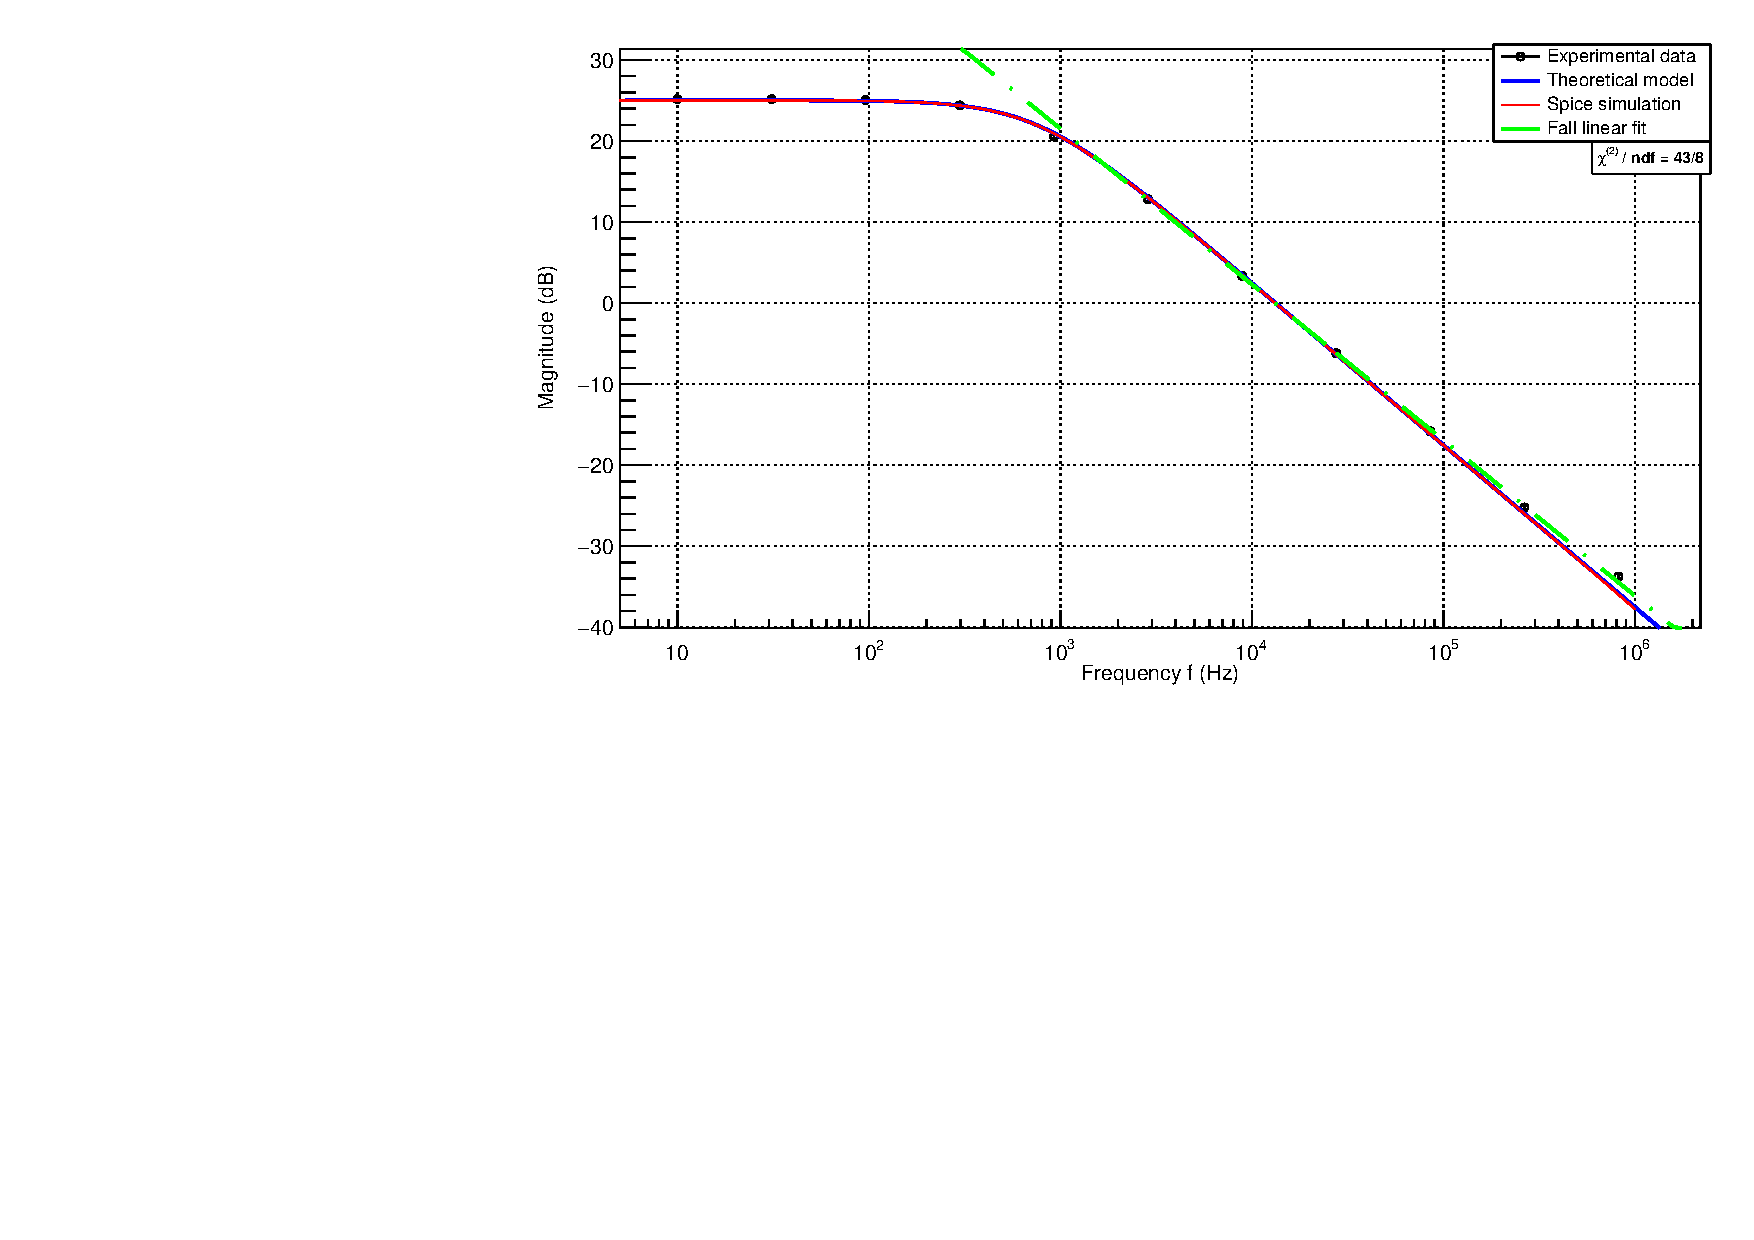
\includegraphics[scale=0.4, angle=0]{bodepreamp.pdf}
        \setlength{\belowcaptionskip}{-20pt}
        \caption{grafico di Bode del circuito preamplificatore}
        \label{fig:bodepreamp}
    \end{figure}
\end{center}



%Si osserva che i dati giacciono correttamente sulla simulazione e anche il modello teorico appare adeguato, nonostante gli ultimi punti si distacchino, seppur in modo
%non notevole, dal grafico. In ogni caso, come si osserva anche dal seguente grafico dei residui, gli errori sono sufficientemente ampi da tenere conto dell'imprecisione
%delle misure a frequenze alte, quando il segnale in uscita si trova all'estremo del range dell'oscilloscopio. Pertanto, il $\chi_{(2)}$ risulta ottimo.

\begin{center}
    \begin{figure}[H]
        \centering
        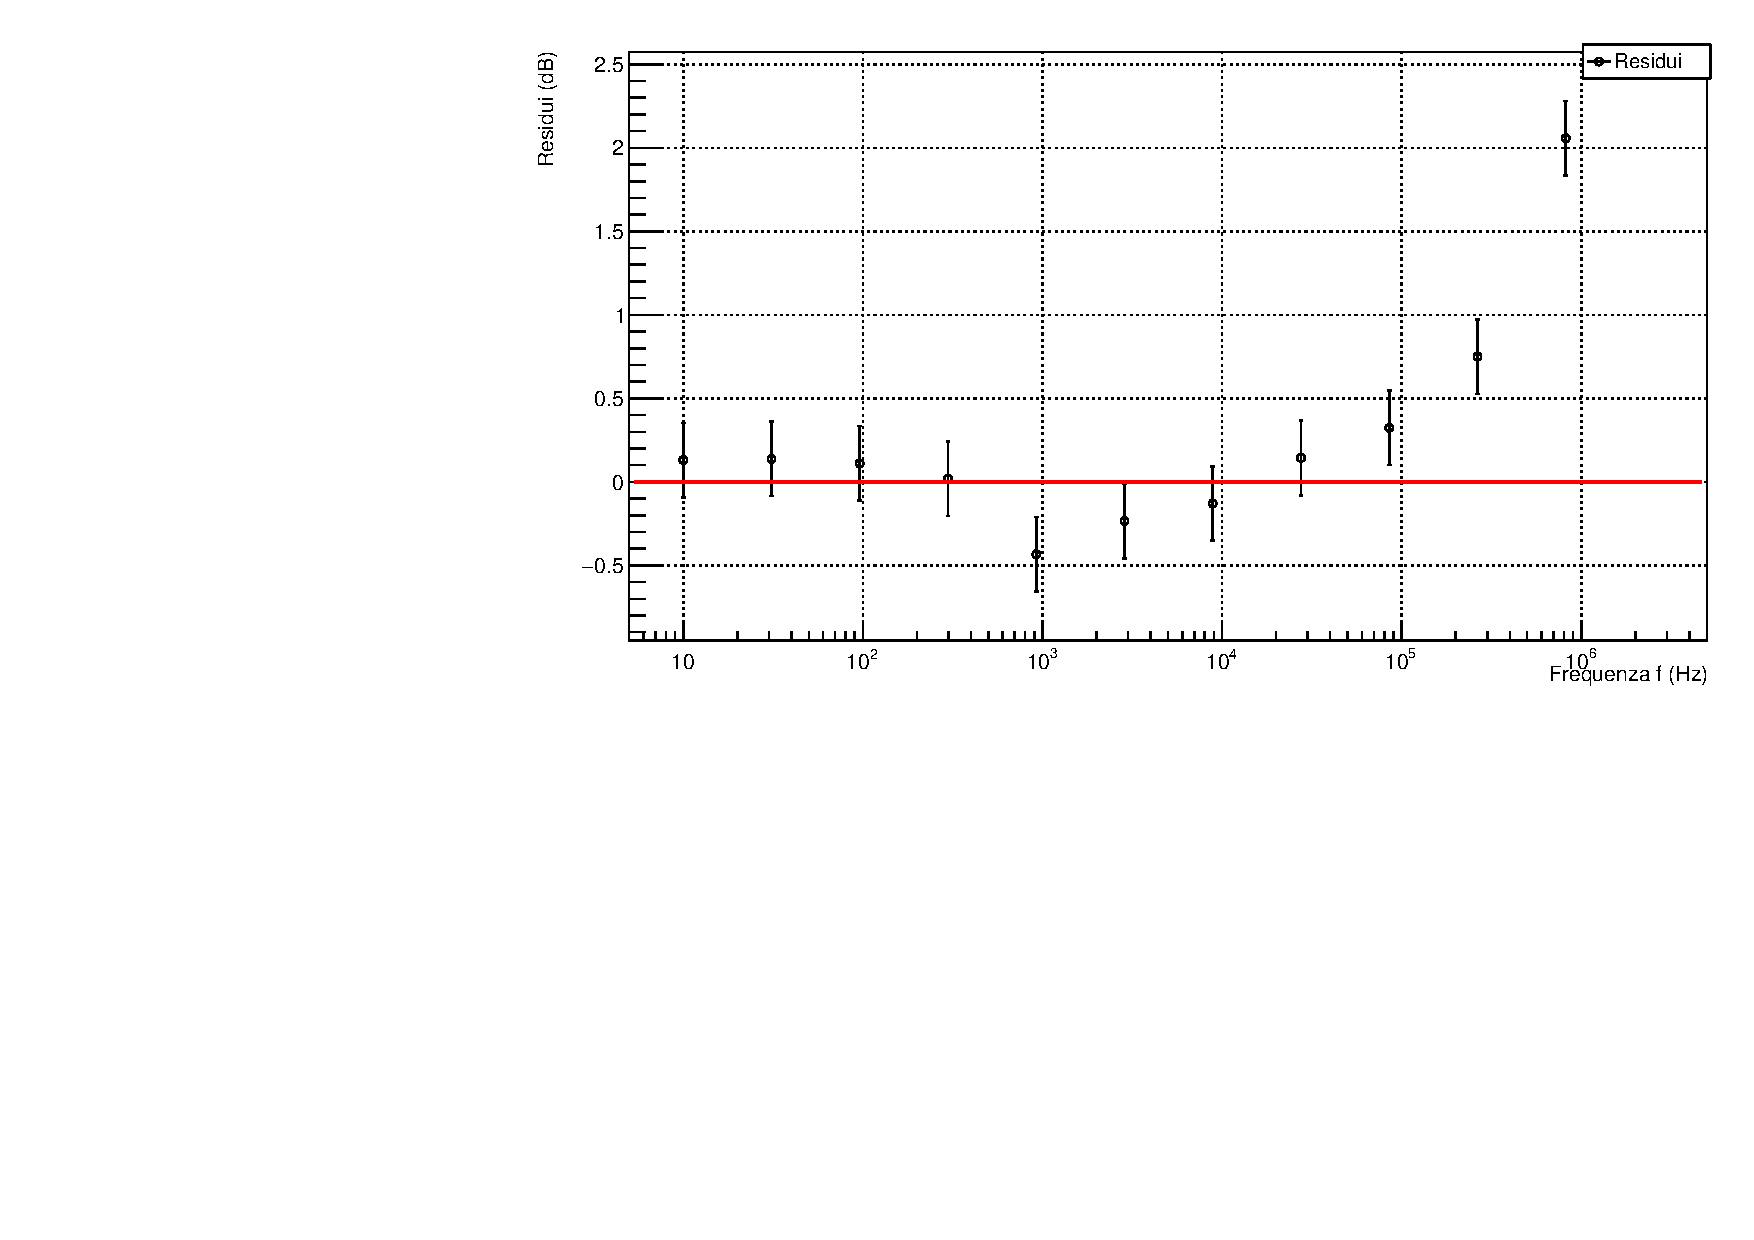
\includegraphics[scale=0.4, angle=0]{bodepreampresidui.pdf}
        \setlength{\belowcaptionskip}{-20pt}
        \caption{residui del grafico di Bode}
        \label{fig:bodepreamp_res}
    \end{figure}
\end{center}

Si osserva che i dati sono rappresentati ottimamente dal modello teorico per basse
frequenze, mentre per alte frequenze tendono a discostarsi, anche in modo 
significativo da esso. Si osserva quindi un valore di $\chi^{(2)} \approx 43$ del tutto 
incompatibile con il suo valore di aspettazione ($gdl = 8$). 

La natura di tali problematiche è da ricercarsi in effetti trascurati, quali capacità parassite della breadboard utilizzata o
altri fenomeni che causano la non idealità dell'esperimento.

Come si può notare in Figura \ref{fig:bodepreamp} si è effettuato anche un
fit lineare della discesa, per verificare che la slope sia effettivamente
compatibile con il valore atteso di $-20 \text{dB}/\text{decade}$. Si ottengono
dunque i seguenti parametri di interpolazione:

\begin{table}[ht]
    \centering
    \begin{tabular}{rcccc}
        \toprule
                &\multicolumn{2}{c}{a$\pm \sigma_a$} &\multicolumn{2}{c}{b$\pm \sigma_b$}\\
                &\multicolumn{2}{c}{(dB)}  &\multicolumn{2}{c}{(dB/decade)}\\
        \midrule
        discesa &\multicolumn{2}{c}{79.1$\pm$0.6}&\multicolumn{2}{c}{-19.2$\pm$0.1}\\
        \bottomrule
    \end{tabular}
    \caption{parametri di interpolazione lineare della discesa}
\end{table}


\begin{center}
        \begin{figure}[H]
            \centering
            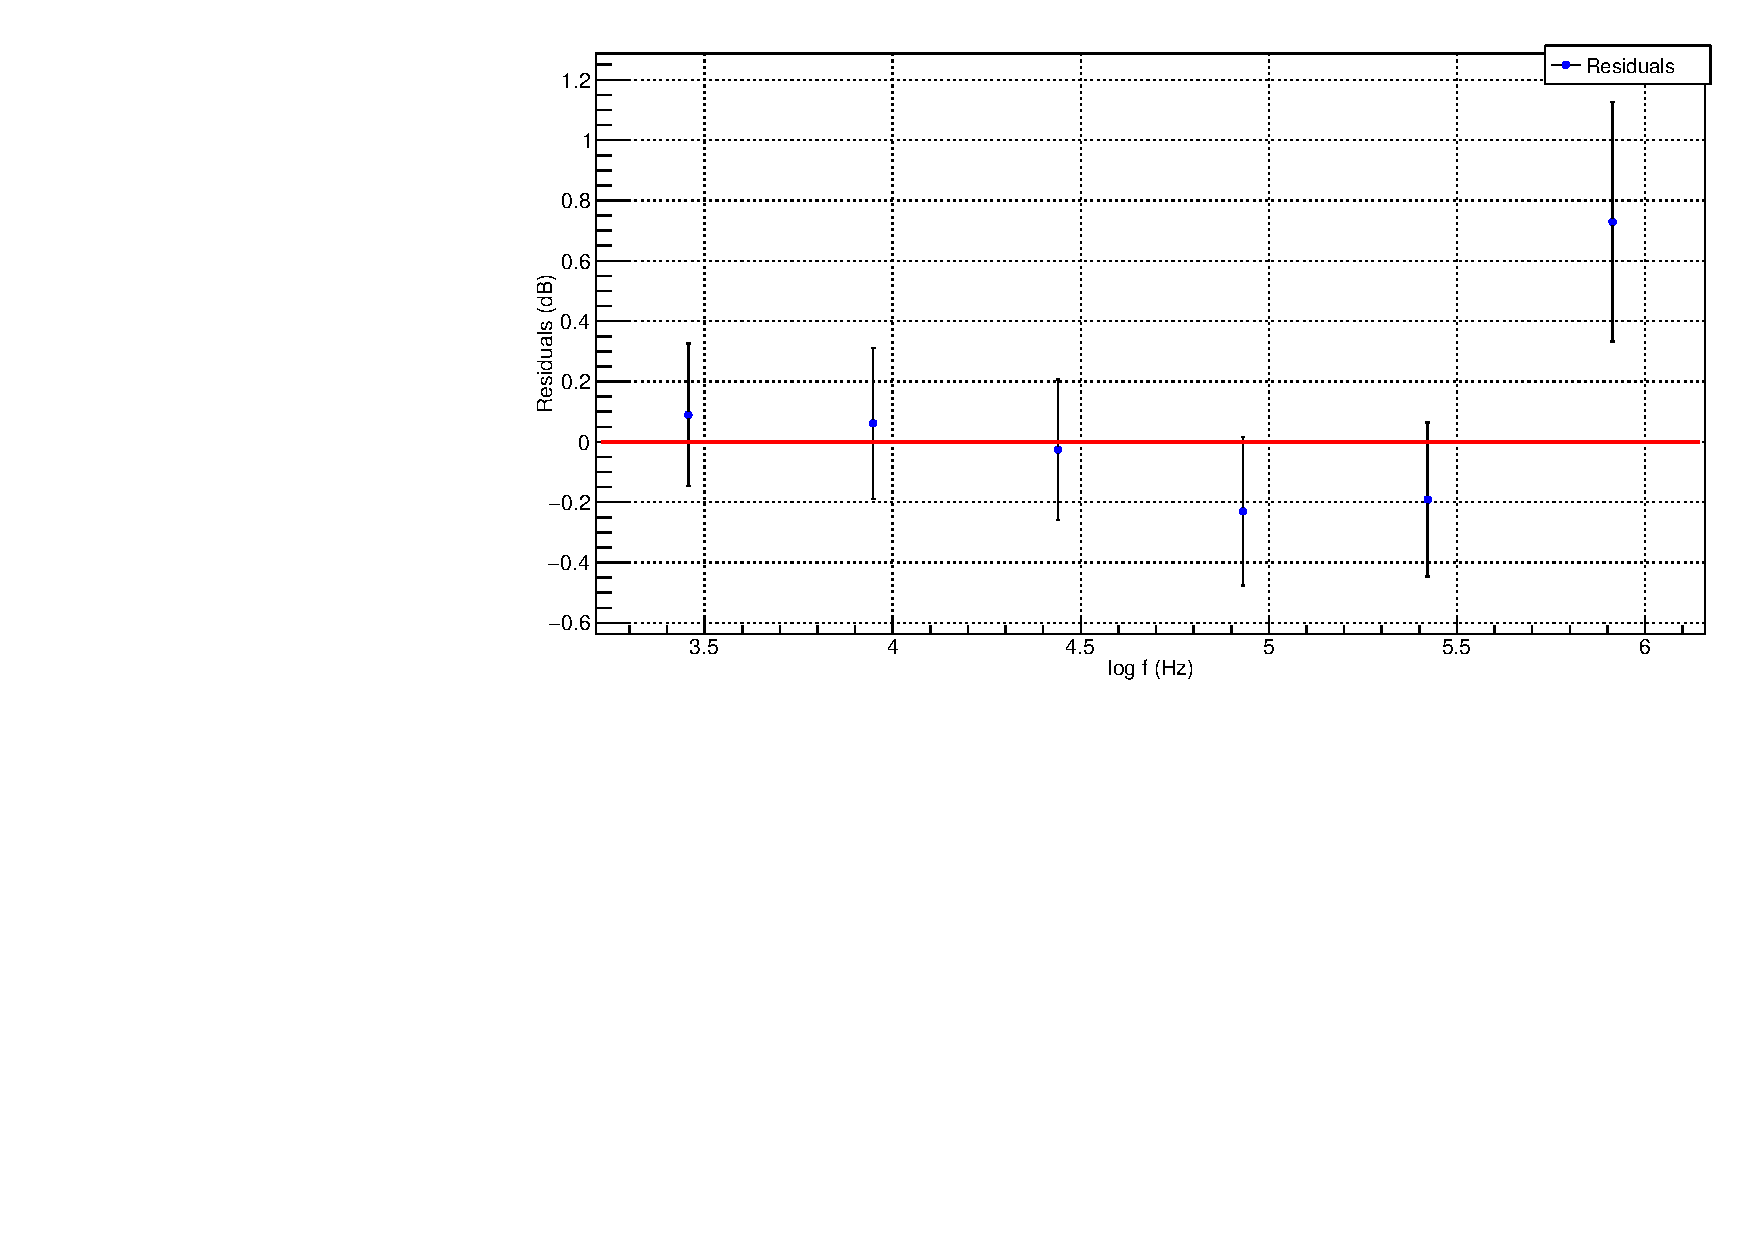
\includegraphics[scale=0.4, angle=0]{residuipreamplineare.pdf}
            \setlength{\belowcaptionskip}{-20pt}
            \caption{residui dell'interpolazione lineare della discesa}
            \label{fig:bodepreamp_res_lineare}
        \end{figure}
\end{center}

Si nota che il valore di slope non è di fatto
compatibile con il valore atteso: questa
problematica potrebbe essere dovuta a una sottostima degli
errori. In alternativa, è possibile che gli ultimi dati possano
avere qualche bias: infatti escludendo questi punti dal fit si
ottiene un valore di pendenza compatibile con il valore di
aspettazione. Si evita tuttavia di scartare dati: si otterrebbe
un set eccessivamente ristretto e soprattutto non si conosce
la natura di questo bias (potrebbe essere dovuto, come già detto, a
capacità parassite non considerate nello studio),
 sarebbe quindi del tutto arbitrario
tralasciare tali punti nell’analisi.

\begin{table}[ht]
    \centering
    \begin{tabular}{ccccc}
        \toprule
        $\sigma_{y, post}$    &$\chi^{(2)}$    &$\lambda_{\chi}$   &$\rho$ &t      \\
        \midrule
        0.4 dB                &5.03            &0.36               &-0.9998&-107.63\\
        \bottomrule
    \end{tabular}
    \caption{parametri di verifica della bontà del fit}
\end{table}
Tutti i parametri di verifica della bontà del fit permettono di accettare
l'ipotesi di linearità dei dati.



\section{Circuito formatore}
\subsection{Shaper base CR-RC}
\subsubsection{Breve discussione del circuito}

Il secondo passo per la costruzione della catena elettronica consiste invece nella costruzione del circuito formatore il cui schema è 
riportato in Figura \ref{fig:shaper}, che plasmi il segnale fornendo tipicamente un profilo gaussiano.

\begin{center}
    \begin{figure}[ht]
        \centering
        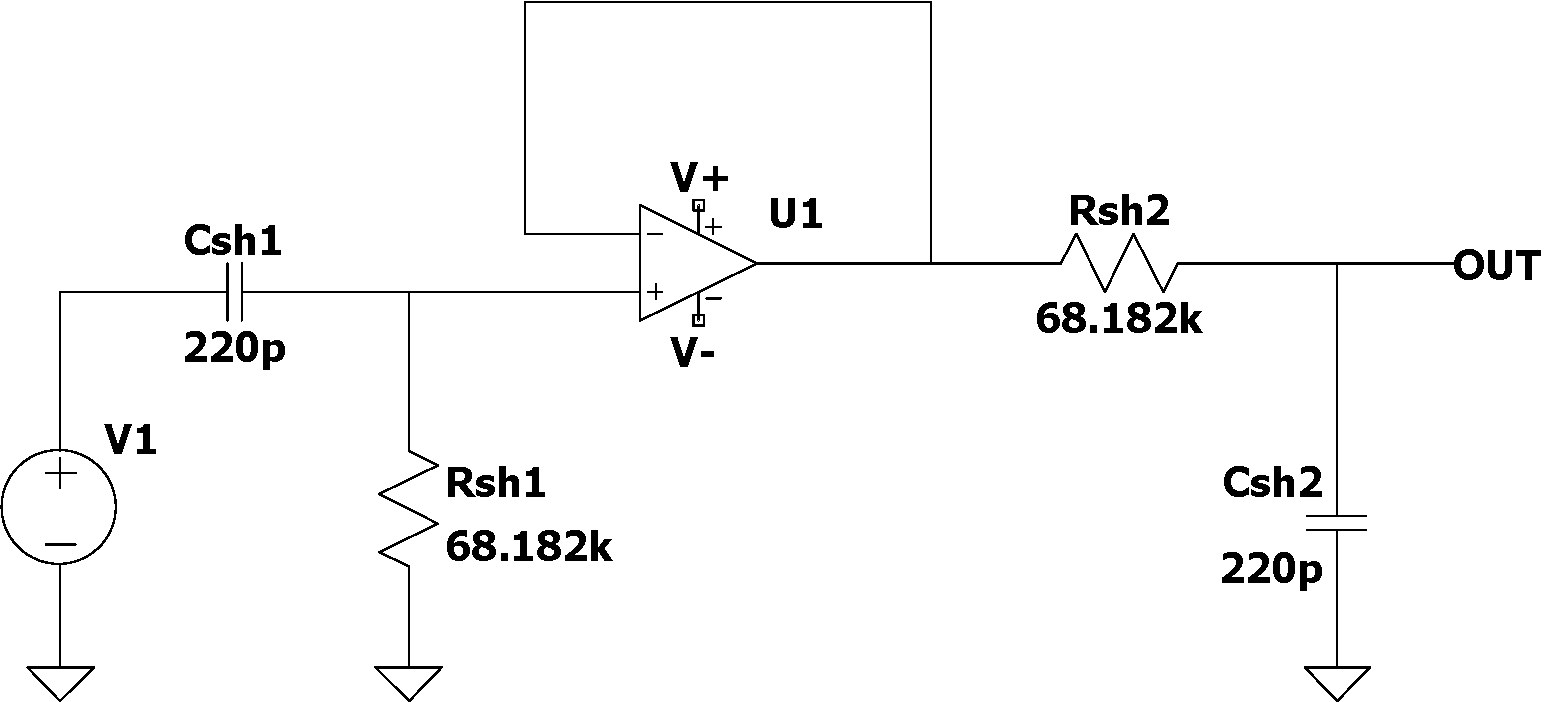
\includegraphics[scale=0.3, angle=0]{shaper.pdf}
        \caption{circuito formatore}
        \label{fig:shaper}
    \end{figure}
\end{center}
    
Si osserva che il circuito è costruito tramite due stadi RC e CR, disaccoppiati tramite un buffer costruito utilizzando il secondo 
opamp presente nel TL082.

Si specifica inoltre che i valori di $C_{sh}^{(1)}\approx C_{sh}^{(2)}$ e $R_{sh}^{(1)}\approx R_{sh}^{(2)}$ sono stati scelti in modo da ottenere 
il valore di $\tau_{sh}$ indicato nel logbook. Tuttavia, a causa di un cambio di combinazione in corso d'opera per problemi sorti durante la 
prima giornata di esperienza, $\tau_{sh}$ e $C_{sh}$ con cui si è lavorato sono sì quelli della nuova combinazione, ma le altre grandezze in gioco sono rimaste quelle
della combinazione originale ($C_{pre,th}=330$ pF, $\tau_{pre}=220$ $\mu s$). Si è utilizzata quindi una capacità di 220 pF
e una costante di tempo caratteristica $\tau_{sh}$ di 15 $\mu s$ che in realtà non sono associati ai parametri usati del preamplificatore in nessuna combinazione.

Trattando il circuito con Laplace e considerando la fase stazionaria, si ottiene che la funzione di trasferimento in funzione di 
$\omega$ è la seguente:
\begin{equation}
H(\omega)=\frac{\omega \tau}{1+\omega^2\tau^2}
\end{equation}
In particolare, inserendo in ingresso un'onda quadra tra 0 e $V_0$ si ottiene la funzione $V_{out}(t)$ facendo l'antitrasformata 
dal dominio delle frequenze:

\begin{equation}
    \label{eqn:V_sh}
    V_{out}(t)= - \frac{V_0}{\tau} t \cdot e^{-\frac{t}{\tau}}
\end{equation}
    

\subsubsection{Discussione dei dati}
Si è nuovamente impostata sul generatore di funzioni un'onda quadra di frequenza di 100 Hz e ampiezza misurata pari a $V_{0}=(992 \pm 15)$mV
in modo che simuli il comportamento di un preamplificatore ideale che mantenga il segnale alto per un tempo indefinito.

Sapendo che $\tau_{th}=R_{sh}^{(1)} C_{sh}^{(1)} = R_{sh}^{(2)} C_{sh}^{(2)}=15 \mu s$ si sono scelti e misurati i seguenti valori:

\begin{align*}
R_{sh}^{(1)} = (68.31  \pm 0.03)k\Omega \quad\quad \sigma_{\%}=  0.04 \% \\
R_{sh}^{(2)} = (68.075  \pm 0.03)k\Omega \quad\quad \sigma_{\%}=  0.04\% \\
C_{sh}^{(1)}= (234 \pm  9)pF \quad\quad \sigma_{\%}= 4 \% \\
C_{sh}^{(2)}= (234 \pm  9)pF \quad\quad \sigma_{\%}= 4 \% \\
\end{align*}
dove l'errore è stato calcolato secondo quanto scritto in appendice. %tenendo conto delle specifiche del multimetro Metrix 32292 relative
%ad un fondoscala di 100 k$\Omega$ per le resistenze e di 1000 pF per le misure delle capacità.

Mediante i cursori si è quindi misurato il valore massimo (in valore assoluto) $V_{sh}^{max}=(346 \pm 6)$mV e il tempo corrispondente 
$\tau_{sh}^{max}=(16 \pm 1)\mu$ s.

Si è poi verificata la correttezza del trasferimento immettendo nel circuito un'onda quadra di ampiezza 1V e misurando un set di 10 punti 
della curva in uscita, indicata dal modello in \ref{eqn:V_sh}. In particolare però per l'identificazione della curva teorica si è 
scelto di non utilizzare il $\tau_{sh}^{sper}$ ma bensì di sfruttarlo come parametro per applicare il metodo del minimo $\chi^{(2)}$, 
ossia vagliare i valori del $\chi^{(2)}$ rispetto ai dati sperimentali al variare di $\tau_{sh}$ e quindi
della curva teorica e poi scegliere il tempo caratteristico per cui l'estimatore risulta avere un minimo. 
La scelta del minimo è stata effettuata tramite un fit parabolico in prossimità della convessità, e calcolando l'ascissa del 
vertice della parabola.
L'errore di $\tau_{sh}$ è dato dalla semidispersione ottenuta facendo riferimento all'intervallo [$\tau_+ ; \tau_-$] 
tali per cui $\chi^{(2)}_{\pm} = \chi^{(2)}_{min} + 1$.

\begin{center}
    \begin{figure}[H]
        \centering
        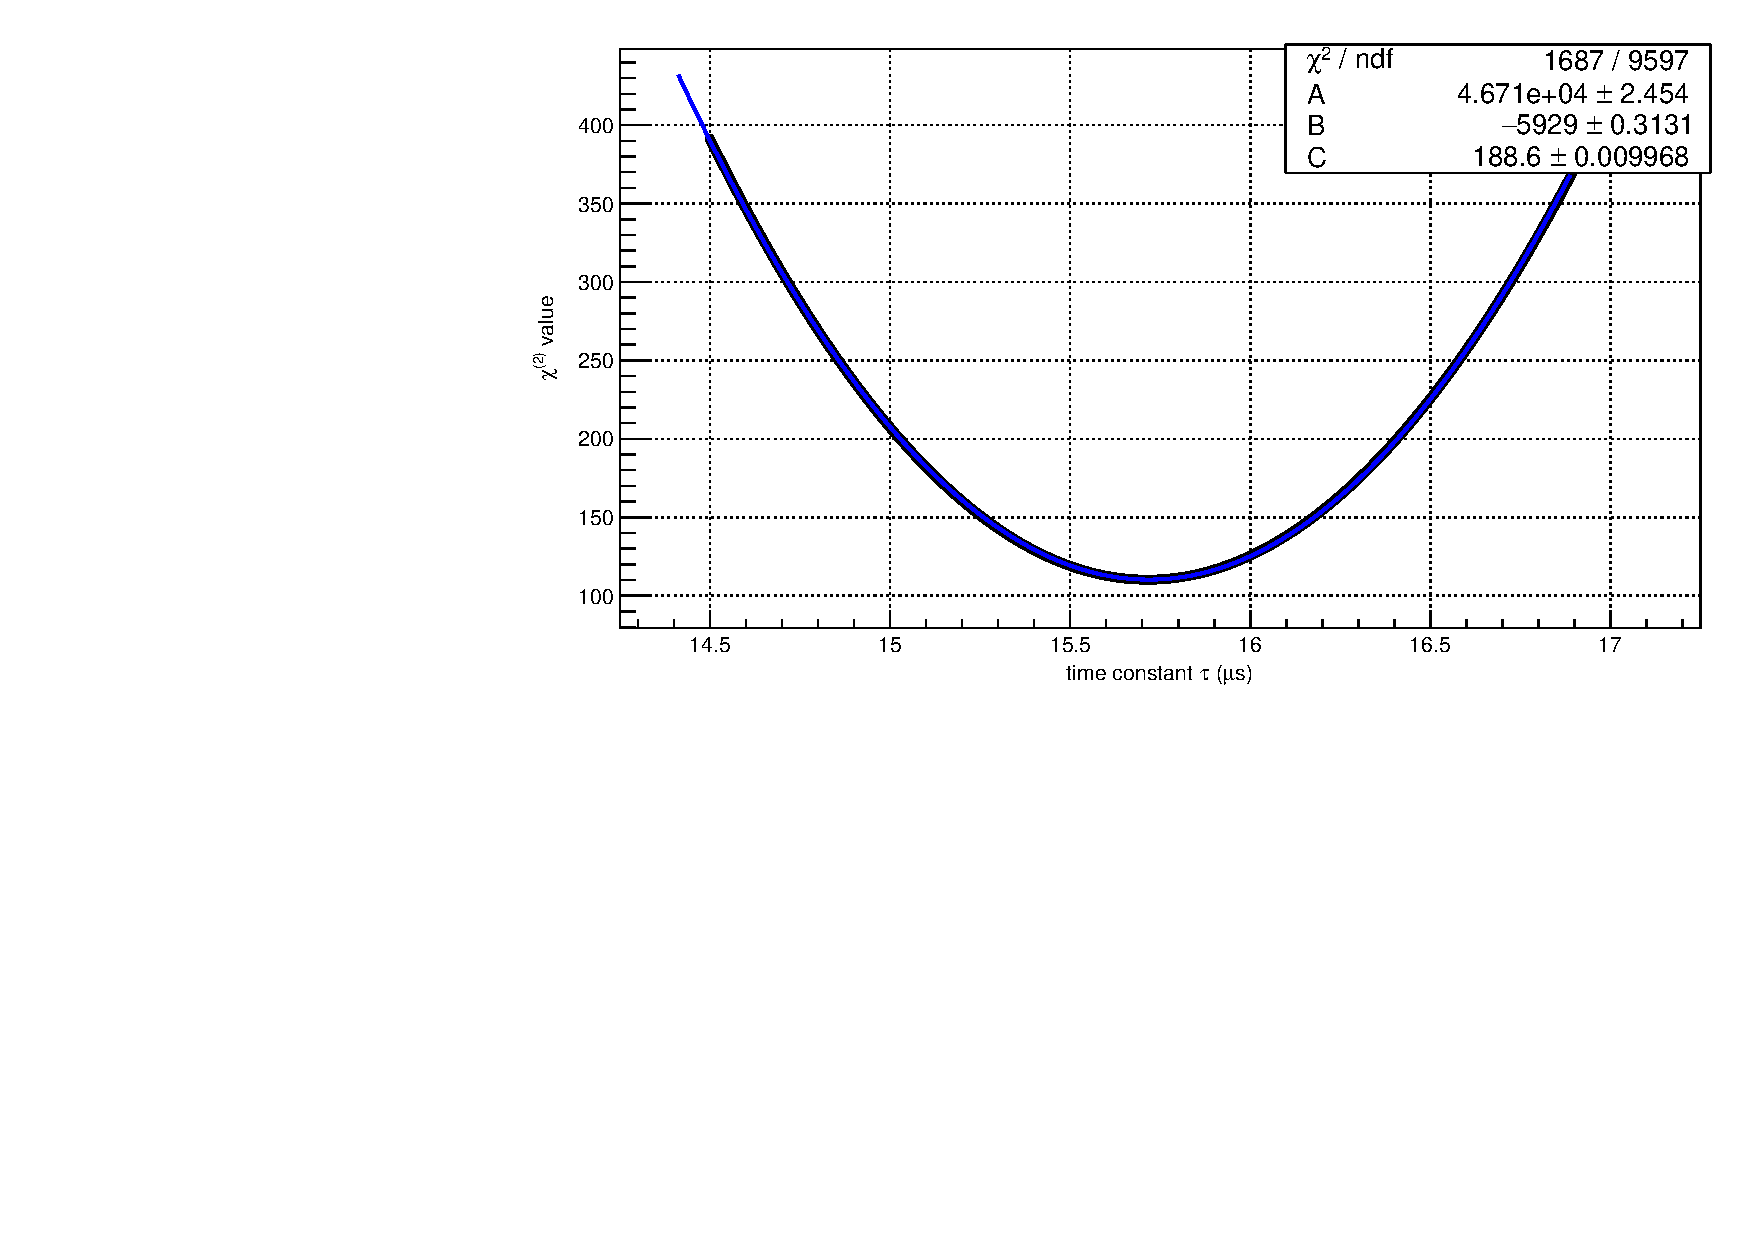
\includegraphics[scale=0.375, angle=0]{chi_forma_no_pz.pdf}
        \setlength{\belowcaptionskip}{-20pt}
        \caption{andamento di $\chi^{(2)}$ al variare di $\tau_{sh}$}
        \label{fig:chi_forma_no_pz}
    \end{figure}
\end{center}
Da cui si sceglie $\tau_{sh} = (15.72\pm 0.07) \mu s$.  Tuttavia si osserva che
il valore di $\chi^{(2)} \approx 110 $ corrispondente è tutt'altro che confortante 
considerando il numero limitato di gradi di libertà. I grafici seguenti
mostrano tale problematica:


\begin{center}
    \begin{figure}[H]
        \centering
        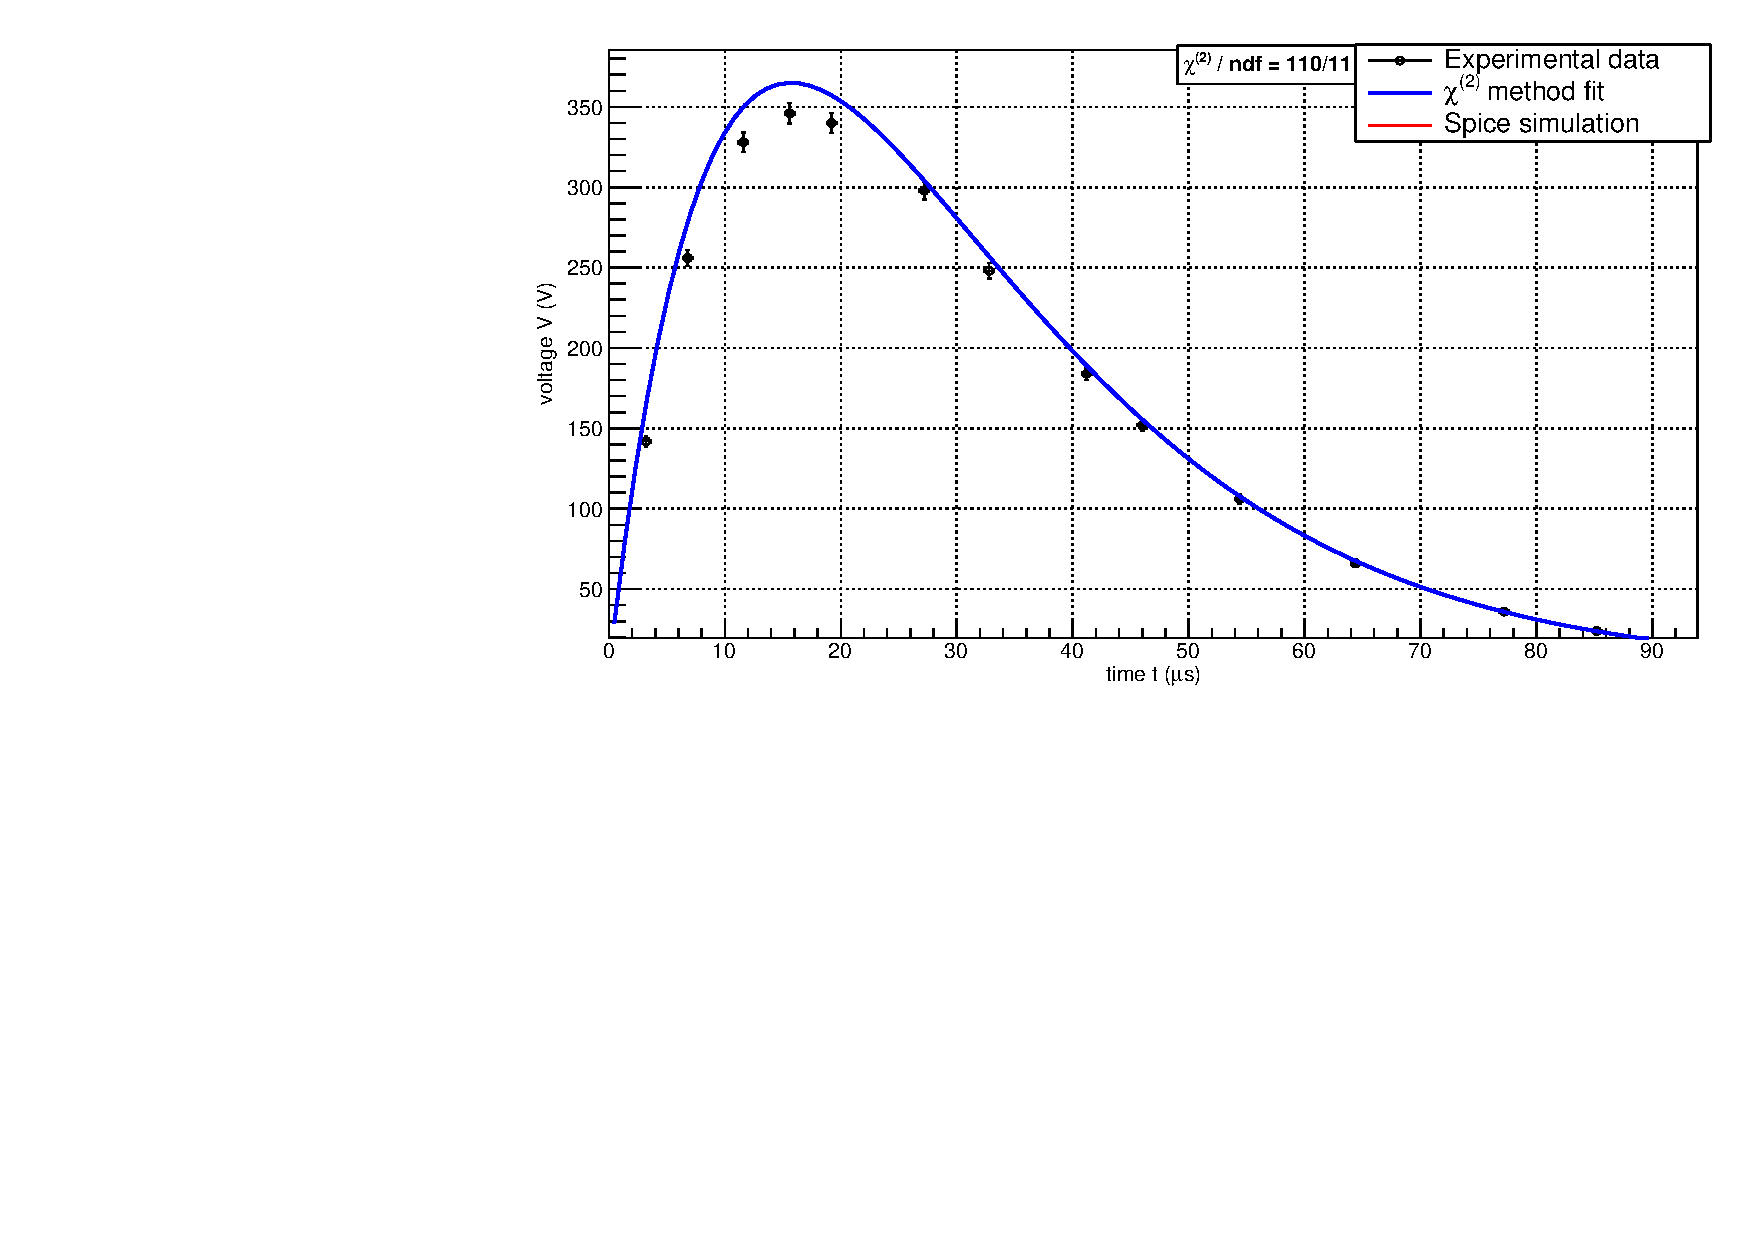
\includegraphics[scale=0.375, angle=0]{forma_no_pz.pdf}
        \setlength{\belowcaptionskip}{-20pt}
        \caption{risposta del circuito formatore a un'onda quadrata in ingresso}
        \label{fig:forma_no_pz}
    \end{figure}
\end{center}

\begin{center}
    \begin{figure}[H]
        \centering
        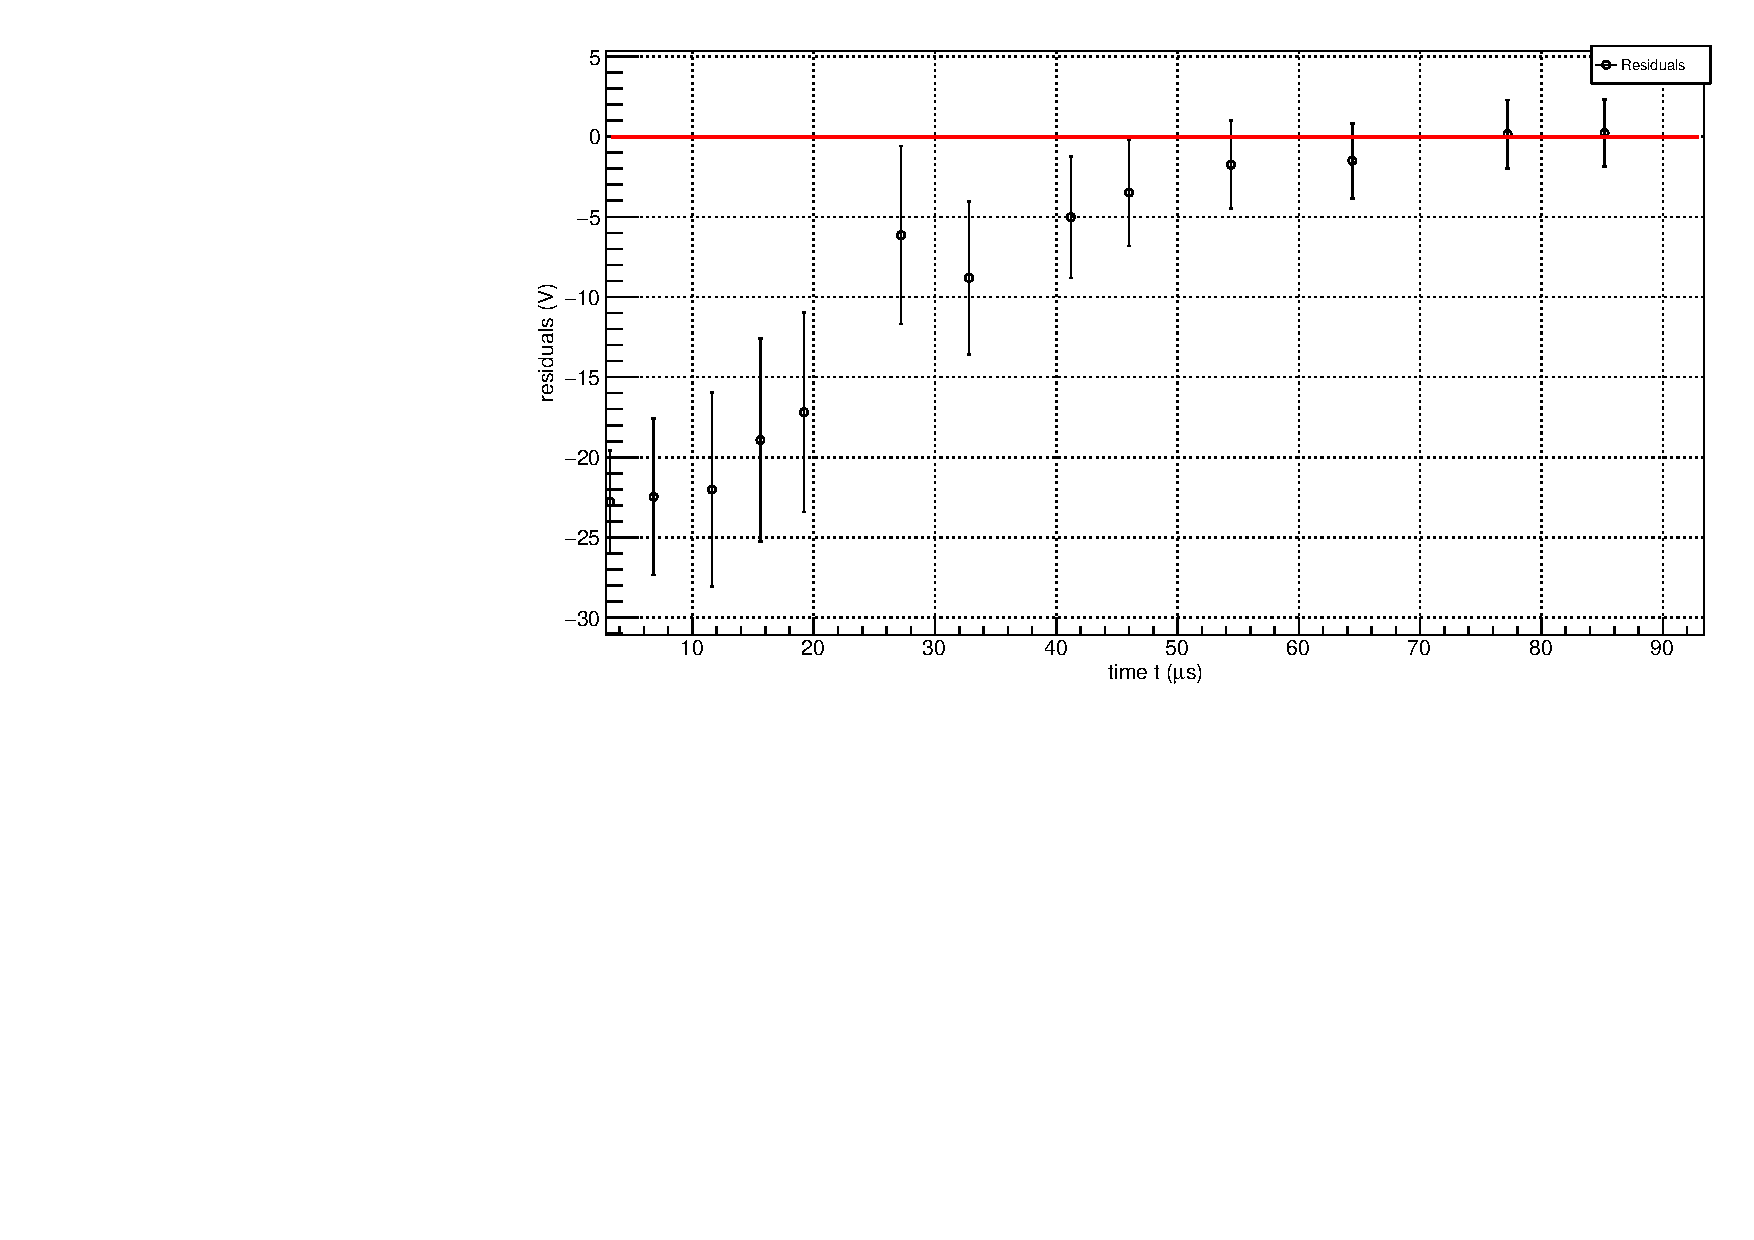
\includegraphics[scale=0.375, angle=0]{residui_forma_onda_no_pz.pdf}
        \setlength{\belowcaptionskip}{-20pt}
        \caption{residui della risposta dello shaper a un'onda quadra}
        \label{fig:forma_no_pz_residui}
    \end{figure}
\end{center}


Si nota che i dati non sono compatibili con il modello teorico, in quanto pur riproducendone l'andamento risultano sensibilmente 
staccati, in particolare in prossimità del picco. La forma \ref{eqn:V_sh} ha massimo in $V_0$/e, ossia il picco è proporzionale all'altezza dell'impulso
inserito, per cui si dovrebbe avere $V_{sh,th}^{max}$ = $(365 \pm 5) mV $, mentre si è misurato  $V_{sh}^{max}=(346 \pm 6)mV$. La compatibilità è $\lambda=2.3$,
accettabile, ma comunque pessima. Da una parte abbiamo quindi il cattivo $\chi^{(2)}$, dall'altra una compatibilità accettabile tra i due picchi: si potrebbe dunque 
sospettare una certa sottostima degli errori, che però non sembra sufficiente a spiegare un tale distacco dei dati dal modello, che sembrerebbe 
sistematico, in quanto i dati tendono a rimanere sempre al di sotto della curva teorica.


%Sembra dunque che nel circuito costruito in laboratorio il segnale erogato dal generatore si attenui leggermente all'ingresso del
%circuito, forse a causa di un settaggio non corretto di \textit{input impedance} nelle opzioni del generatore di funzioni  ????

Come anticipato, il valore di $\chi^{(2)}$ ottenuto porta a dover rifiutare il 
fit. Dal grafico dei residui si osserva la tendenza per la quale 
ai tempi iniziali la curva risulta completamente inadatta, mentre sulla coda descrive bene
i dati.

Osservando anche la curva ottenuta dalla simulazione spice si nota che 
essa risulta molto fedele alla curva ottenuta con il fit, quindi il problema
sembrerebbe essere sui dati.

Tale problematica potrebbe essere riconducibile ad un errore umano, dovuto a impostazioni sbagliate nell'onda in ingresso,
come ad esempio l'ampiezza dell'onda, o in alternativa
a qualche bias dovuta ancora alla non idealità del circuito.
 
\medskip

Si è infine nuovamente studiato il comportamento del circuito al variare della frequenza. Si è 
ottenuto il seguente grafico di Bode (Figura \ref{fig:bodeshaper_no_pz}), al fine di ottenere un confronto immediato sono plottate 
sovrapposte la curva teorica relativa ai dati sperimentali ed il fit dei dati ottenuti mediante la simulazione di LTspice:

\begin{center}
    \begin{figure}[H]
        \centering
        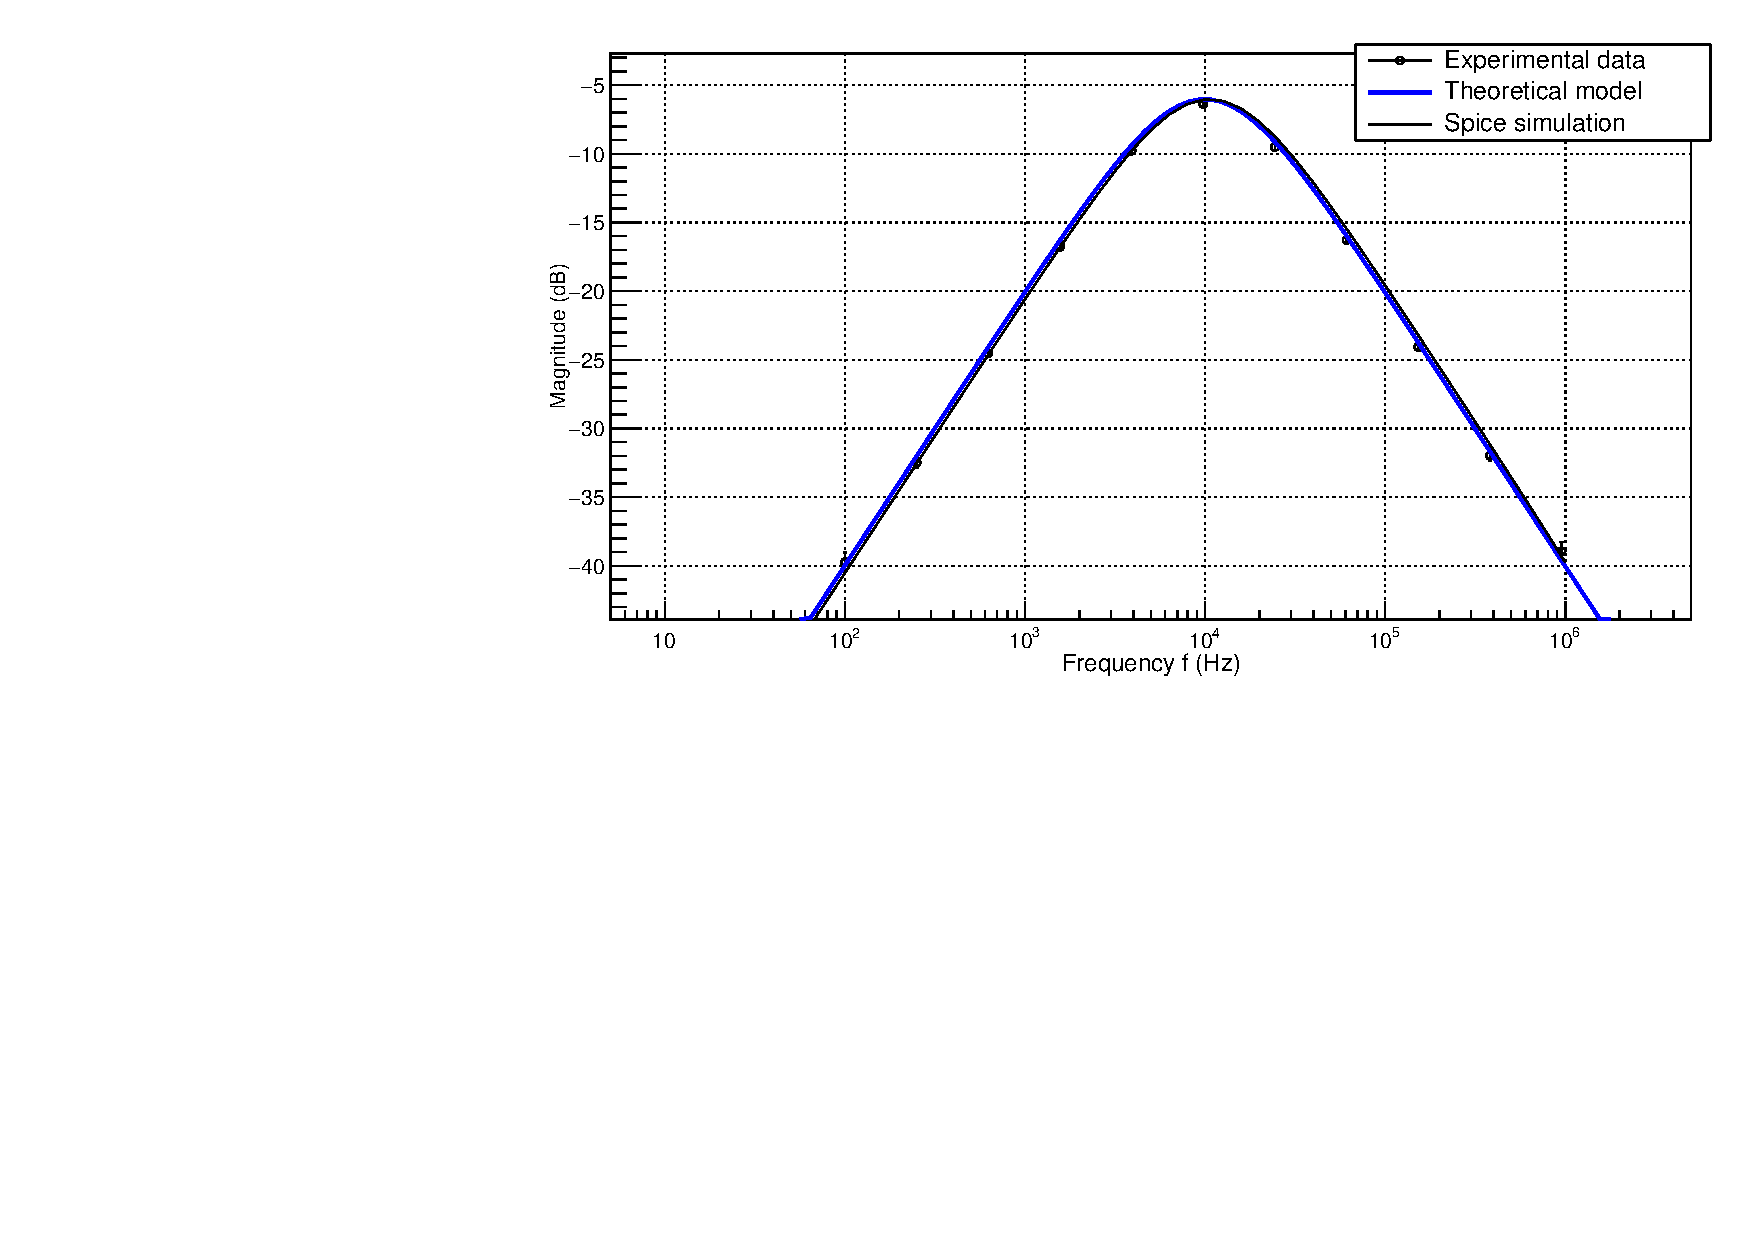
\includegraphics[scale=0.375, angle=0]{bodeshaper_no_pz.pdf}
        \setlength{\belowcaptionskip}{-40pt}
        \caption{grafico di Bode del circuito formatore}
        \label{fig:bodeshaper_no_pz}
    \end{figure}
\end{center}

\begin{center}
    \begin{figure}[ht]
        \centering
        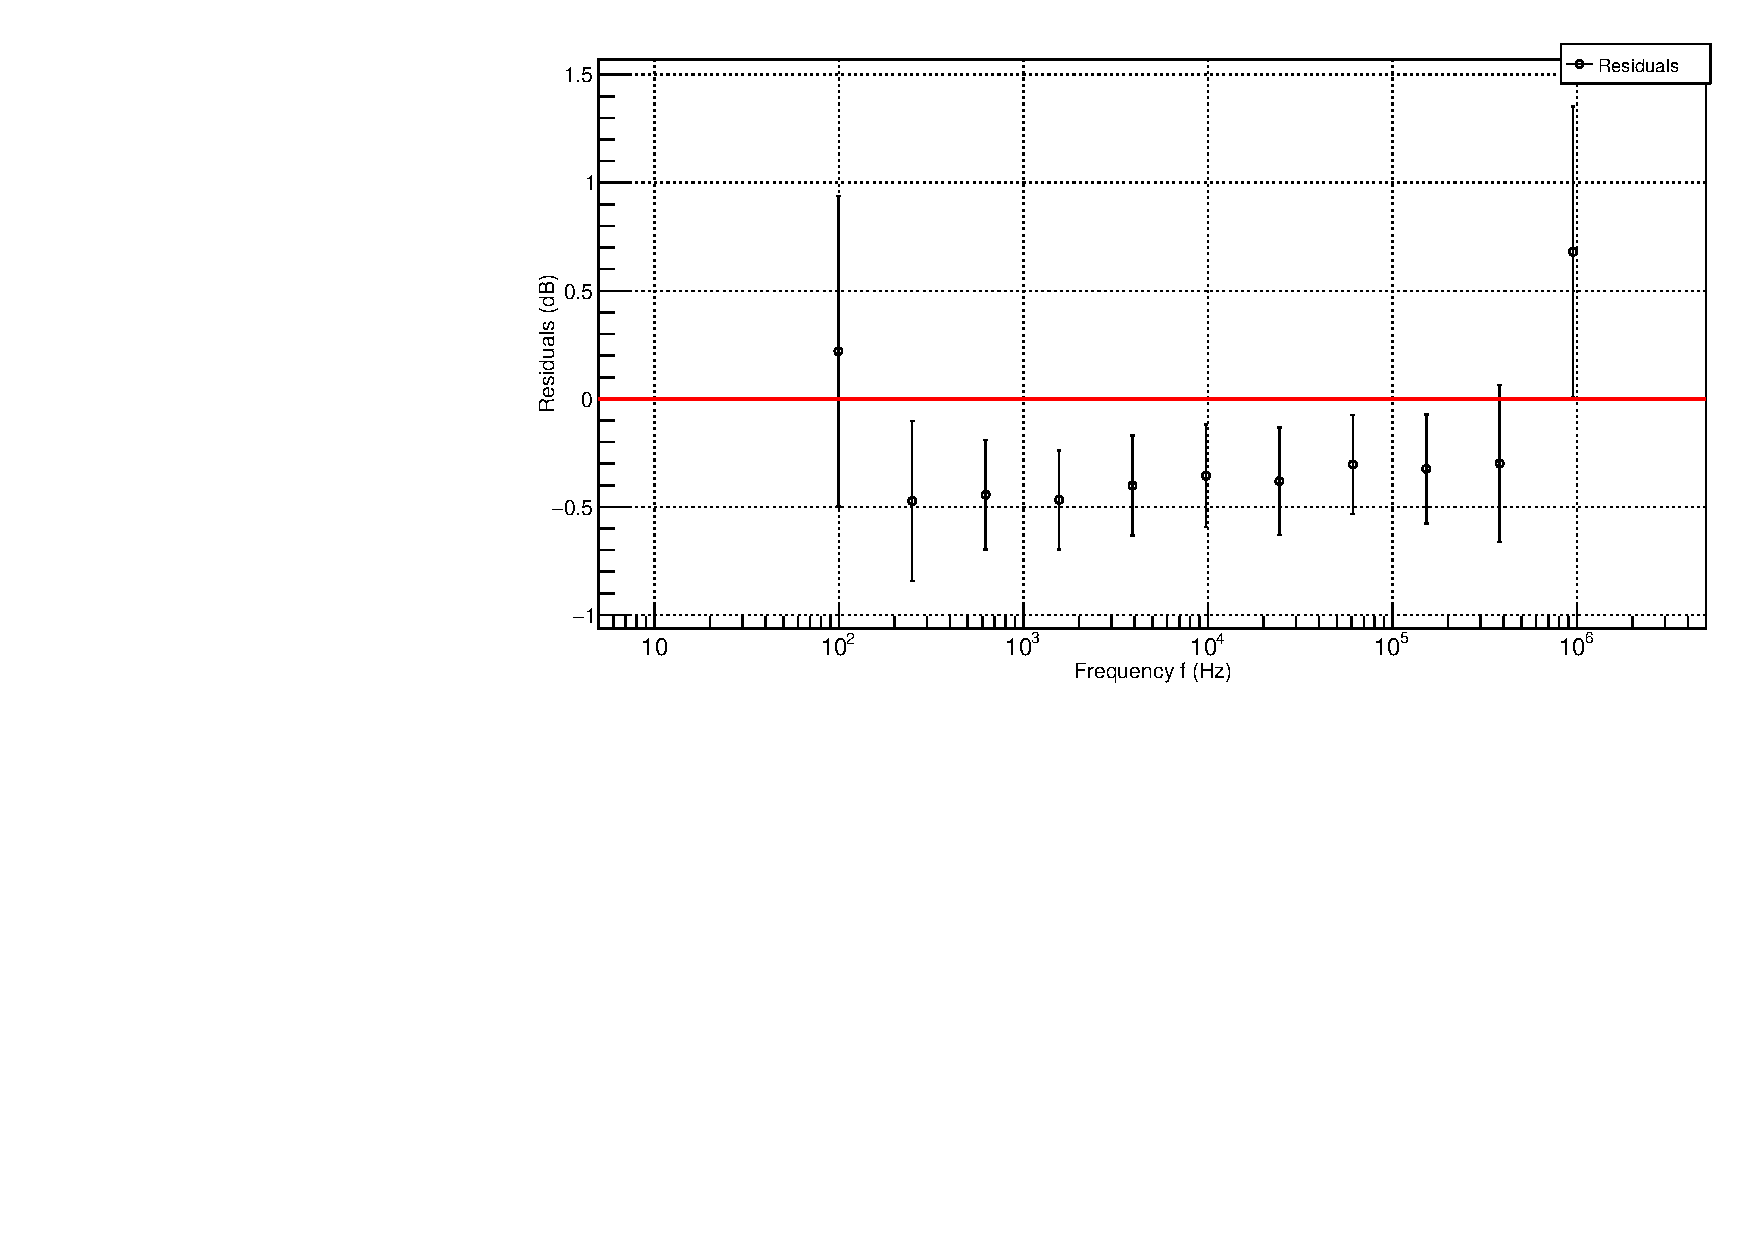
\includegraphics[scale=0.3875, angle=0]{bodeshaperresidui_no_pz.pdf}
        \setlength{\belowcaptionskip}{-20pt}
        \caption{ residui del grafico di Bode }
        \label{fig:bodeshaperresidui_no_pz}
    \end{figure}
\end{center}


Si osserva il diverso comportamento dello shaper base, che opera come derivatore per frequenze basse e come integratore a frequenze
alte.

Il valore di $\chi^{(2)}$ risulta compatibile con il suo valore di aspettazione, in accordo con la Tabella \ref{tab:compatibilità}.
Tuttavia si nota in Figura \ref{fig:bodeshaperresidui_no_pz} una certa sistematicità: la curva tende
a rimanere sempre sopra ai dati.

Come si osserva in Figura \ref{fig:bodeshaper_no_pz} si sono effettuati i fit della salita e della discesa,
per la verifica della consistenza delle pendenze.


\begin{table}[ht]
    \centering
    \begin{tabular}{rcccc}
        \toprule
                &\multicolumn{2}{c}{a$\pm \sigma_a$} &\multicolumn{2}{c}{b$\pm \sigma_b$}\\
                &\multicolumn{2}{c}{(dB)}  &\multicolumn{2}{c}{(dB/decade)}\\
        \midrule
        salita  &\multicolumn{2}{c}{-79$\pm$1}&\multicolumn{2}{c}{19.5$\pm$0.4}\\
        discesa &\multicolumn{2}{c}{77$\pm$2}&\multicolumn{2}{c}{-19.4$\pm$0.4}\\
        \bottomrule
    \end{tabular}
    \setlength{\belowcaptionskip}{-20pt}
    \caption{parametri di interpolazione della salita e della discesa}
\end{table}

\begin{figure}[H]
    \centering
    \subfloat[][\emph{Residui fit della discesa}]
        {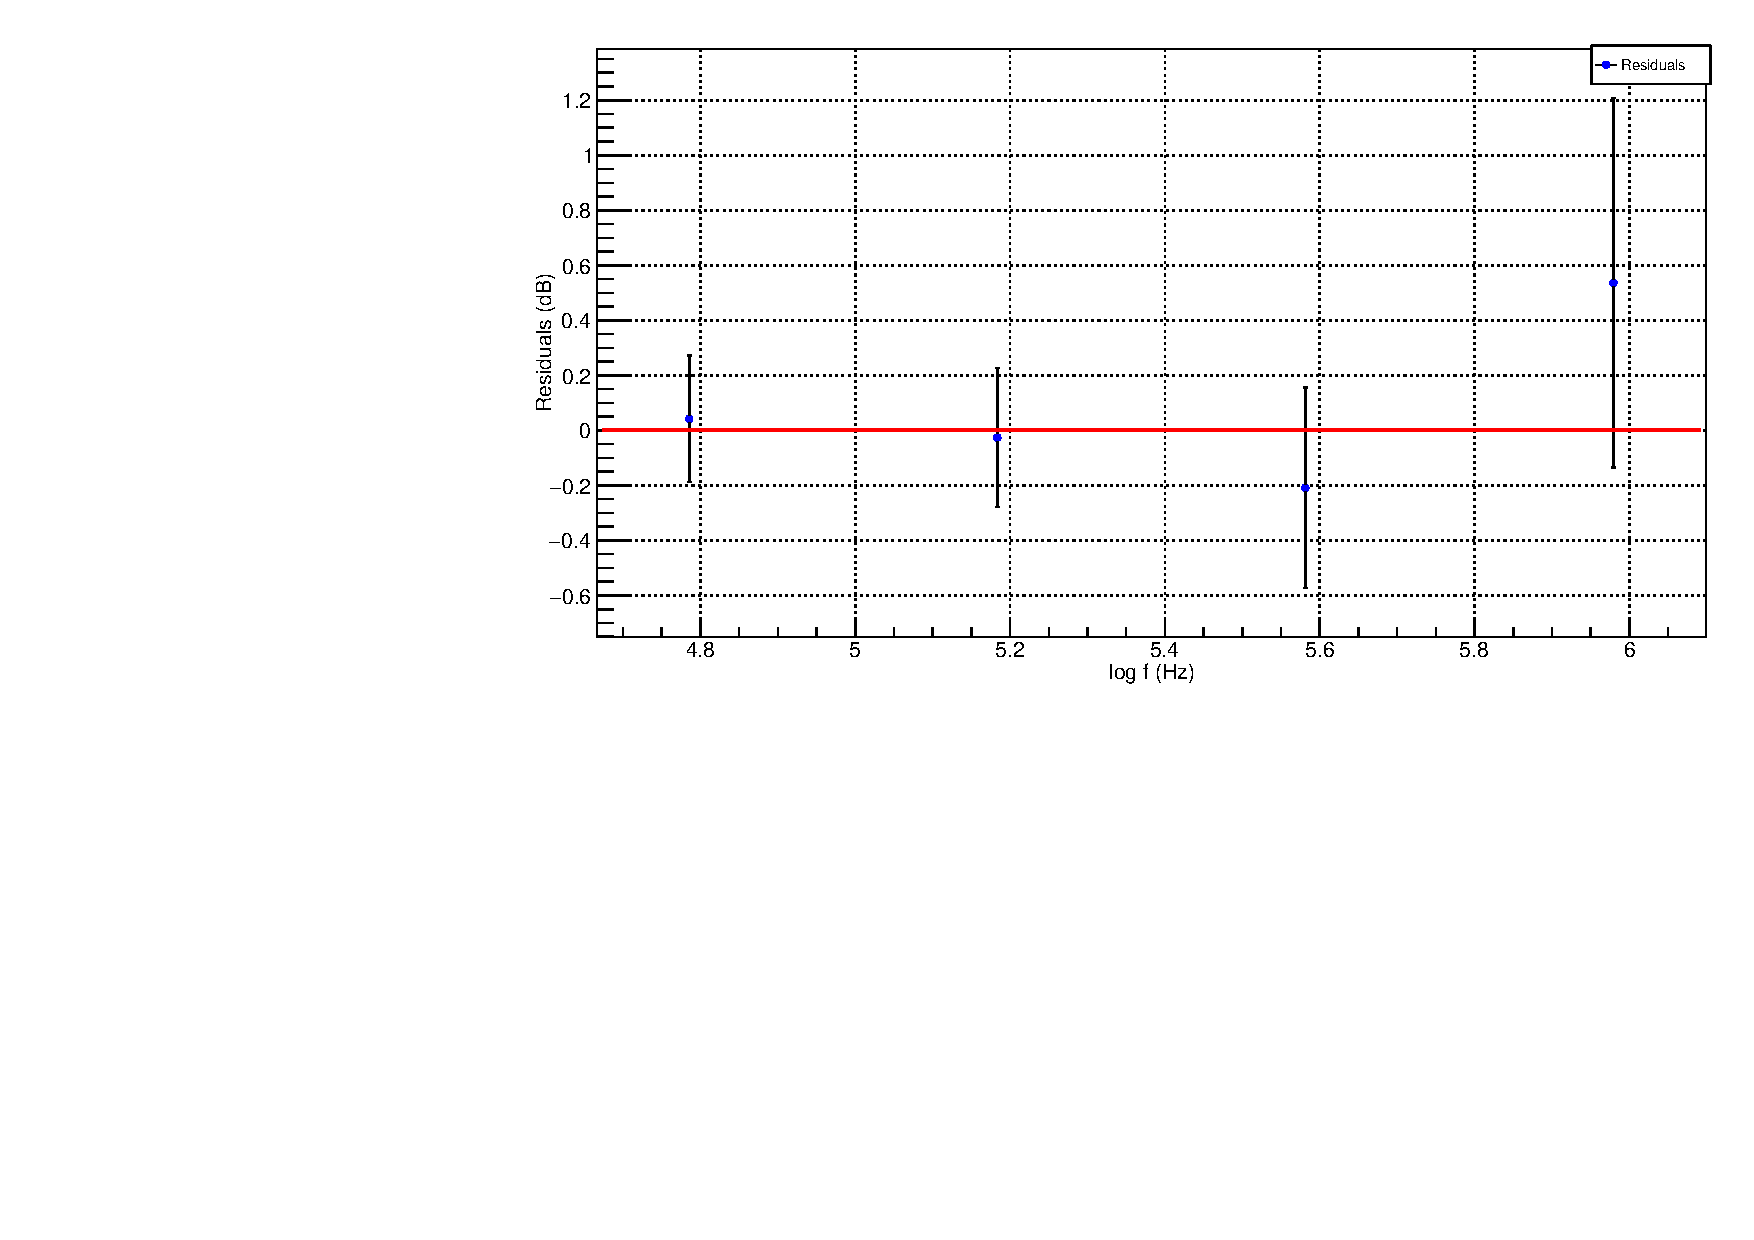
\includegraphics[width=.23\textwidth]{residuishaperdiscesa.pdf}} 
    \subfloat[][\emph{Residui fit della salita}]
        {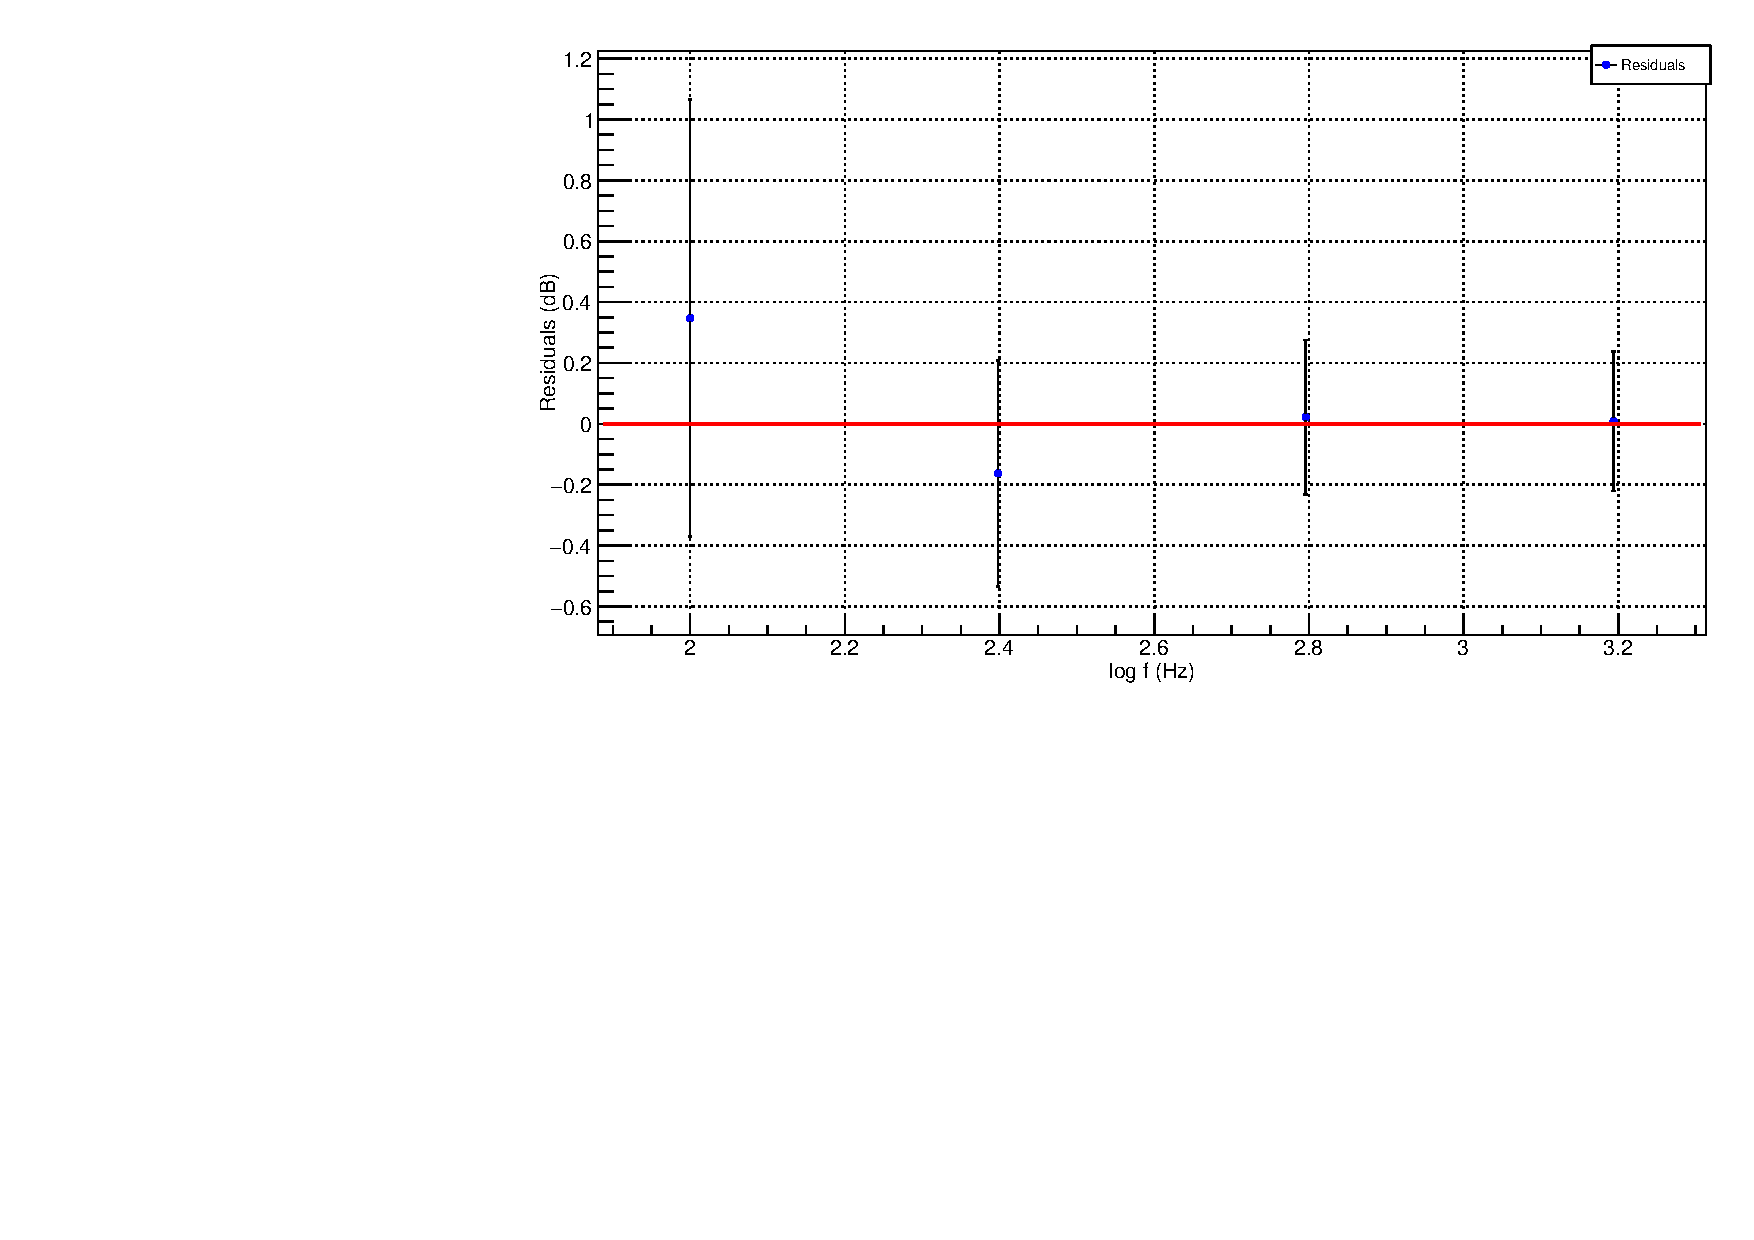
\includegraphics[width=.23\textwidth]{residuishapersalita.pdf}}
    \caption{residui per i fit lineari dello shaper}
    \label{fig:residuishapersladis}
\end{figure}

\begin{table}[H]
    \centering
    \begin{tabular}{cccccc}
        \toprule
                &$\sigma_{y, post}$    &$\chi^{(2)}$    &$\lambda_{\chi}$   &$\rho$ &t      \\
        \midrule
        discesa &0.4 dB                &1.01            &0.49               &-0.9996&-51.23\\
        salita  &0.3 dB                &0.44            &0.78               &0.9998 &76.28  \\
        \bottomrule
    \end{tabular}
    \caption{parametri di verifica della bontà del fit}
\end{table}

Si osserva che i valori di slope osservati sono compatibili con i valori attesi e i parametri di verifica
della bontà del fit permettono tutti di accettare l'ipotesi di andamento lineare.

\subsection{Shaper compensato}

\subsubsection{Breve discussione del circuito}

Si è proceduto inserendo come segnale in ingresso dello shaper il segnale di uscita del preamplificatore. Subentra quindi il problema 
di dover compensare l'effetto del pole-zero: infatti, se si considera in ingresso un segnale del tipo 
\[V_{in}(t)=V_0 e^{-\frac{t}{\tau_{pre}}}\] 
si ottiene la seguente trasformata di Laplace:
\begin{equation}
    V_{in}(s)=\frac{Vo}{s+\frac{1}{\tau_{pre}}}
\end{equation}
che presenta un polo in $-\frac{1}{\tau_{pre}} $,  responsabile dell’undershoot del segnale.

Si osserva però che il segnale in uscita dal primo stadio (CR) del formatore con una tensione in ingresso a gradino è descritto dalla seguente formula: 
$V_{out}(s)^{CR}=\frac{V_{0}}{s+\frac{1}{\tau_{sh}}}$;
si vuole quindi modificare il circuito in modo che all'ingresso del buffer arrivi un segnale che segua questo stesso andamento.
Si è quindi inserita una resistenza $R_{pz}$ in parallelo a $C_{sh}^{(1)}$ e si è studiato l'andamento di $ V_{out}(s)^{CR}$ di questo nuovo circuito mediante la trasformata di Laplace:


\begin{equation}
    V_{out}(s)^{CR}=\frac{V_{0}}{s+\frac{1}{\tau_{pre}}}\cdot \frac{s+\frac{1}{\tau_{pz}}}{s+\frac{1}{\tau_{\parallel}}}
\end{equation}


dove $\tau_{pz}= C_{sh}^{(1)}R_{pz}$, $\tau_{\parallel}= C_{sh}^{(1)}R_{\parallel}$ e $R_{\parallel}$ è il parallelo di $R_{sh}^{(1)}$ e $R_{pz}$;
l’effetto del polo del preamplificatore è quindi annullato con quello dello zero del CR compensato nel caso in cui $\tau_{sh}=\tau_{pz}$ .
Regolando quindi opportunamente tale valore si compensa l'effetto pole-zero;
 si è quindi scelto 
$$R_{pz}= \frac{\tau_{pre}}{C_{sh}^{(1)}}$$



Si riporta quindi di seguito lo schema del circuito dello shaper compensato:
\begin{center}
    \begin{figure}[H]
        \centering
        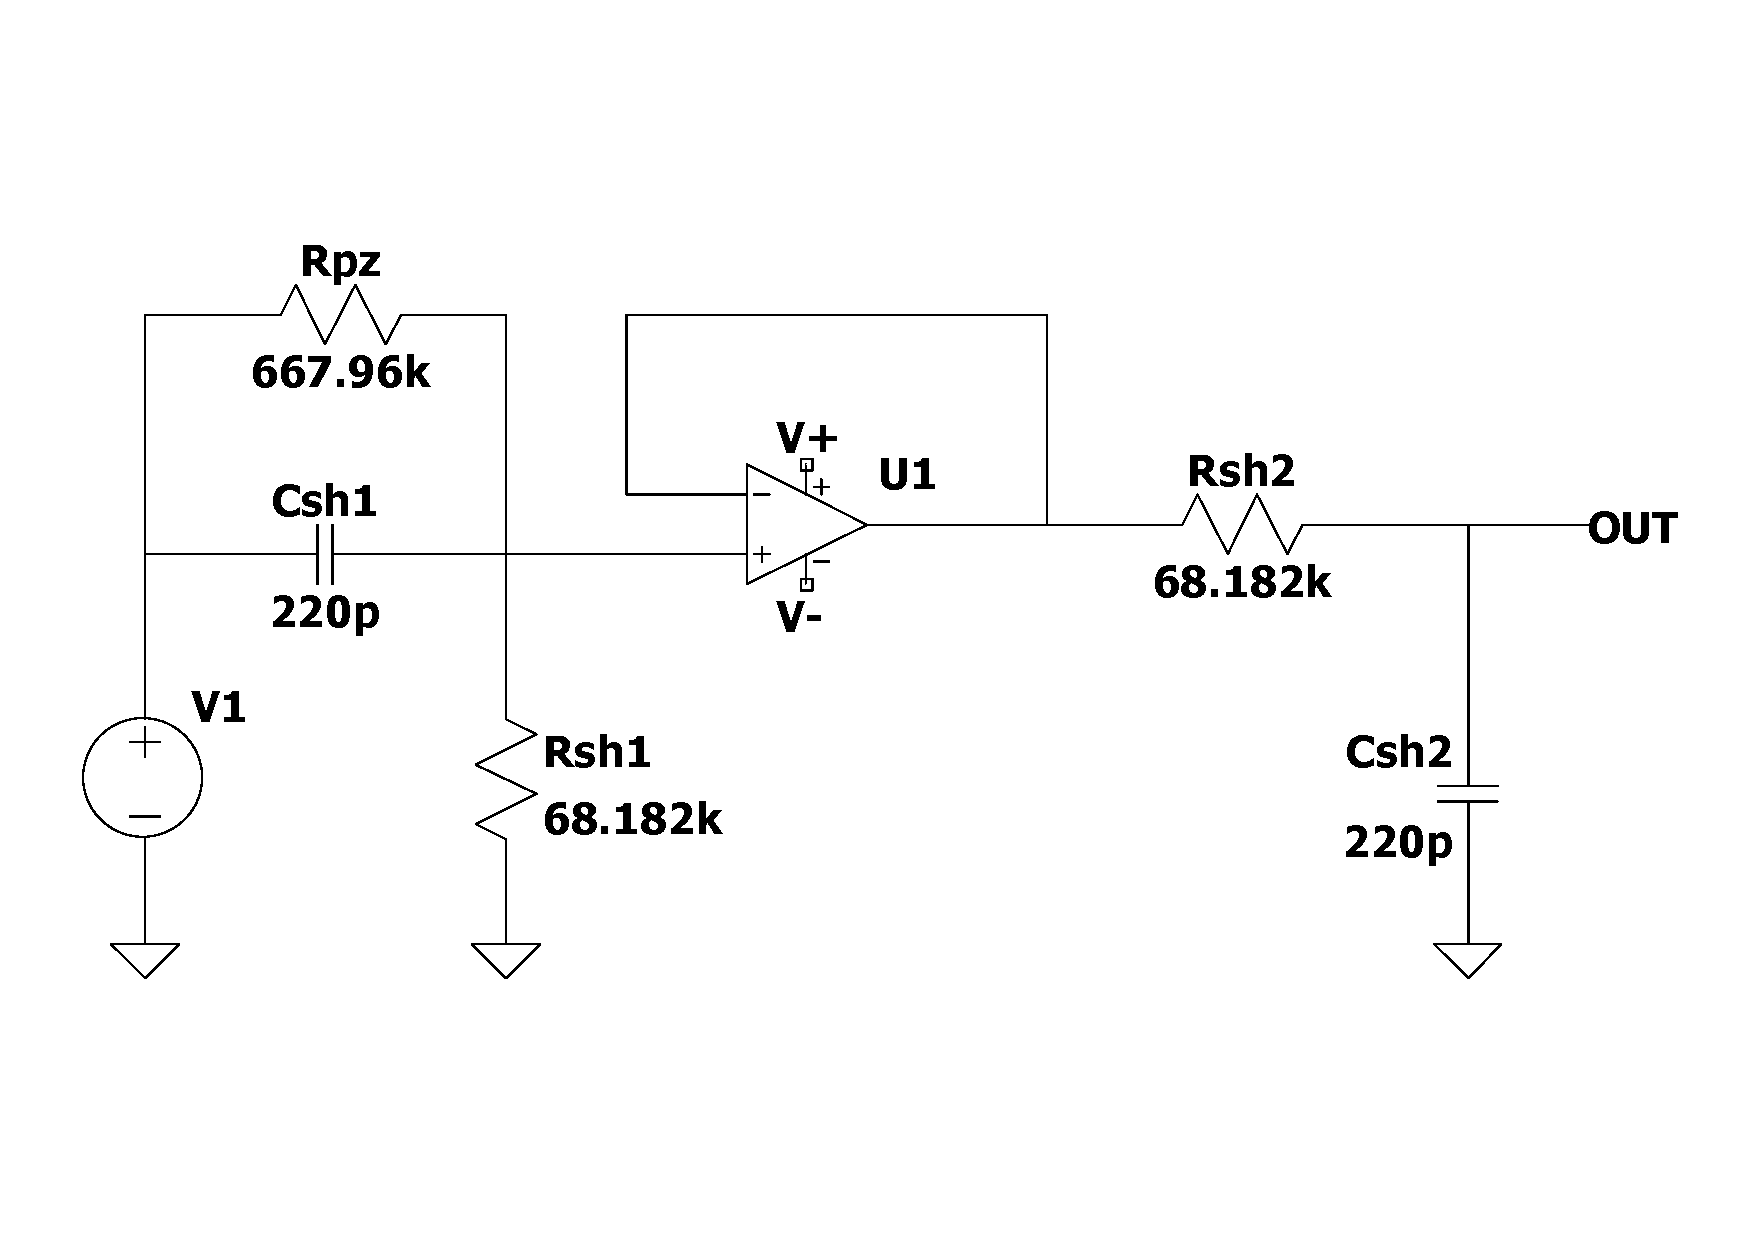
\includegraphics[scale=0.3, angle=0]{shapercomp.pdf}
        \setlength{\belowcaptionskip}{-20pt}
        \caption{circuito formatore con compensazione}
        \label{fig:shaper_pz}
    \end{figure}
\end{center}
dove $V_1$ è il segnale in uscita dal preamplificatore.

Studiando infine la funzione di trasferimento dell'intero circuito  mediante la trasformata di Laplace e passando al dominio delle frequenze con la sostituzione $s\xrightarrow[]{} i\omega$ si ottiene:

\begin{multline}
    \label{eqn:shapercomp_trasf}
    |H(\omega)| =\sqrt{\frac{1}{1+(\omega\tau)^2}\cdot \frac{(R_{sh}^{(1)})^2+(R_{pz}\omega\tau)^2 }{(R_{sh}^{(1)}+R_{pz})^2+(R_{pz}\omega\tau)^2}}
\end{multline}

\subsubsection{Discussione dei dati}

Si è osservato che senza utilizzare lo shaper base per un segnale esponenziale come quello fornito dal preamplificatore si ottiene il 
fenomeno dell'undershoot: infatti unendo preamplificatore e shaper si è misurato $V_{sh, undershoot}=(346 \pm 6)mV$ (l'undershoot è positivo poichè
il segnale è ribaltato a causa della natura invertente del preamplificatore). Inserendo invece la resistenza 
$R_{pz} = (668.0 \pm 3) k\Omega$ si vede che l'effetto di undershoot sparisce e il segnale si adagia correttamente sullo zero 
delle tensioni.

Con il circuito correttamente compensato, si è verificato che la relazione tra carica iniettata e tensione in uscita fosse
lineare, variando la durata dell'impulso in ingresso e acquisendo i picchi delle forme d'onda semigaussiane in uscita dallo shaper.

\begin{center}
    \begin{figure}[H]
        \centering
        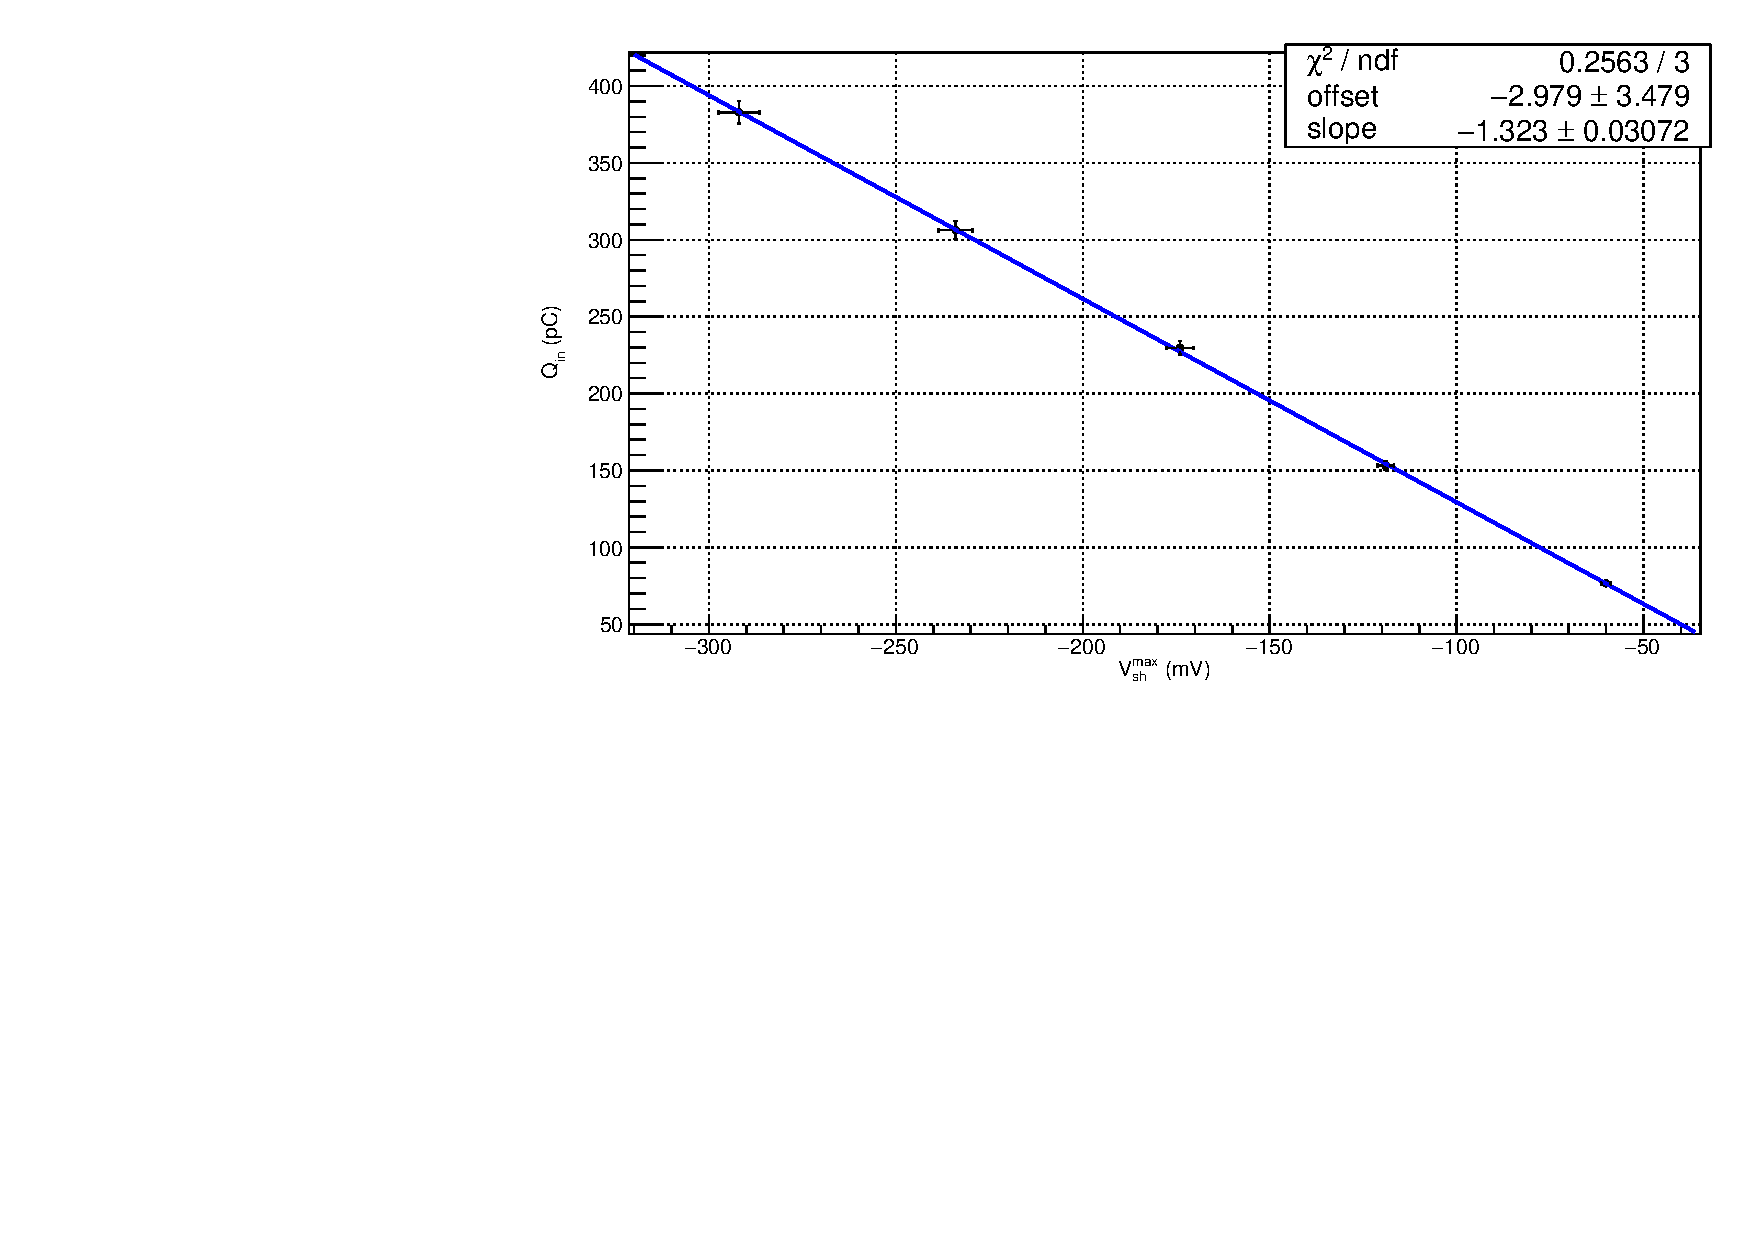
\includegraphics[scale=0.375, angle=0]{fitshaper.pdf}
        \setlength{\belowcaptionskip}{-20pt}
        \caption{carica iniettata e picco di tensione in uscita}
        \label{fig:fitshaper}
    \end{figure}
\end{center}

\begin{center}
    \begin{figure}[H]
        \centering
        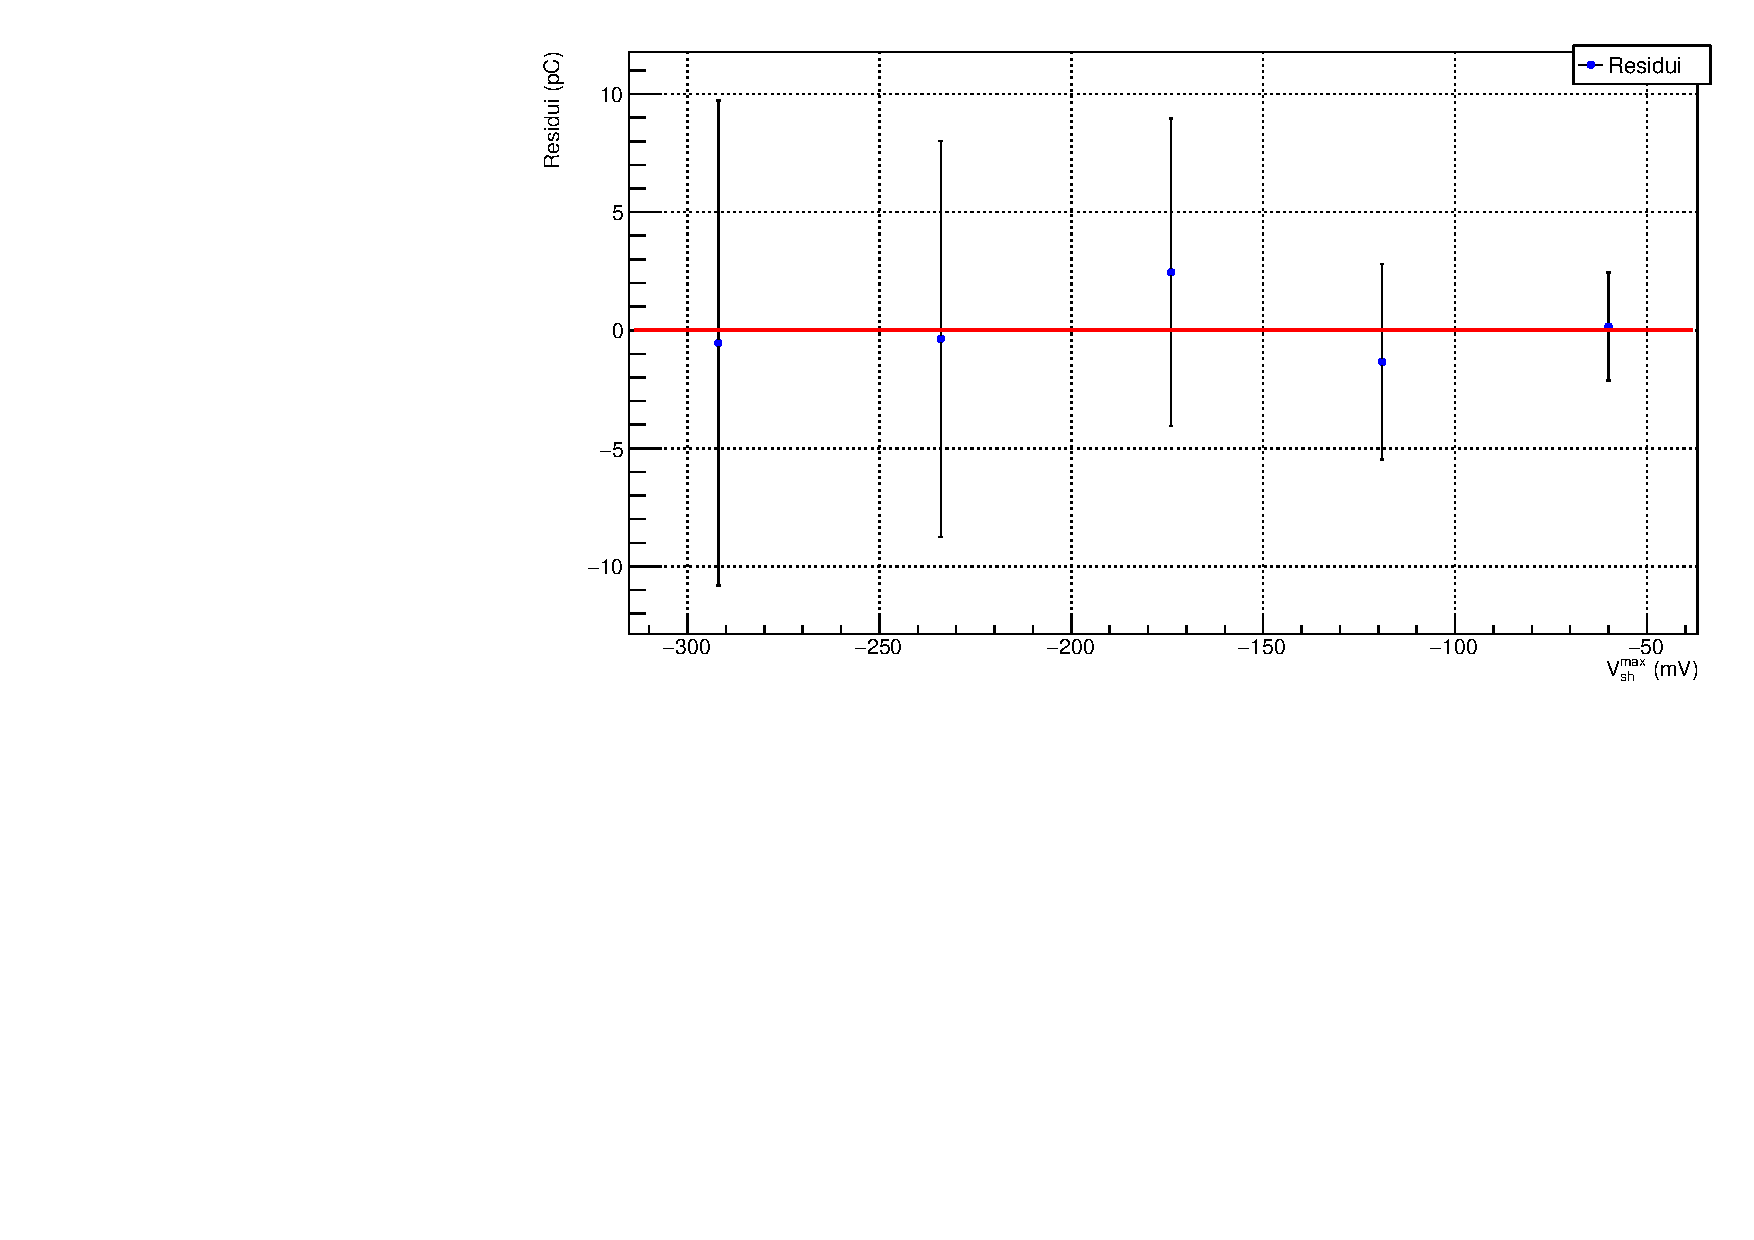
\includegraphics[scale=0.375, angle=0]{residuishaper.pdf}
        \setlength{\belowcaptionskip}{-20pt}
        \caption{grafico dei residui della relazione tra $Q_{in}$ e $V_{pre}^{max}$}
        \label{fig:residuishaper}
    \end{figure}
\end{center}

\begin{table}[ht]
    \centering
    \begin{tabular}{ccccc}
        \toprule
        $\sigma_{y, post}$    &$\chi^{(2)}$    &$\lambda_{\chi}$   &$\rho$  &t   \\
        \midrule
        1.7 V               &0.26            &1.12              &-0.99993&-146.28\\
        \bottomrule
    \end{tabular}
    \caption{parametri di verifica della bontà del fit}
\end{table}

I parametri confermano la buona riuscita del fit lineare e dunque costituiscono la prova della relazione lineare che intercorre tra
carica iniettata e uscita dello shaper.


\section{Circuito amplificatore invertente}

\subsection{Descrizione del circuito}

Unendo il circuto preamplificatore con il circuito formatore otteniamo un segnale correttamente processato ma negativo e dunque non
adatto all'acquisizione da parte di Arduino. Pertanto implementiamo un circuito amplificatore invertente, in particolare un
amplificatore di strumentazione. Tale apparato consiste di un opamp alimentato nell'ingresso invertente, capace dunque di cambiare
segno al segnale, preceduto da un buffer, che ha la funzione di garantire un'alta impedenza di ingresso: infatti con il solo 
amplificatore invertente il segnale cadrebbe sulla resistenza $R_{1a}$, mentre grazie alla presenza dell'inseguitore di tensione 
l'impedenza di ingresso è l'impedenza interna dell'opamp $U_1$, che si può considerare infinita.

\begin{center}
    \begin{figure}[H]
        \centering
        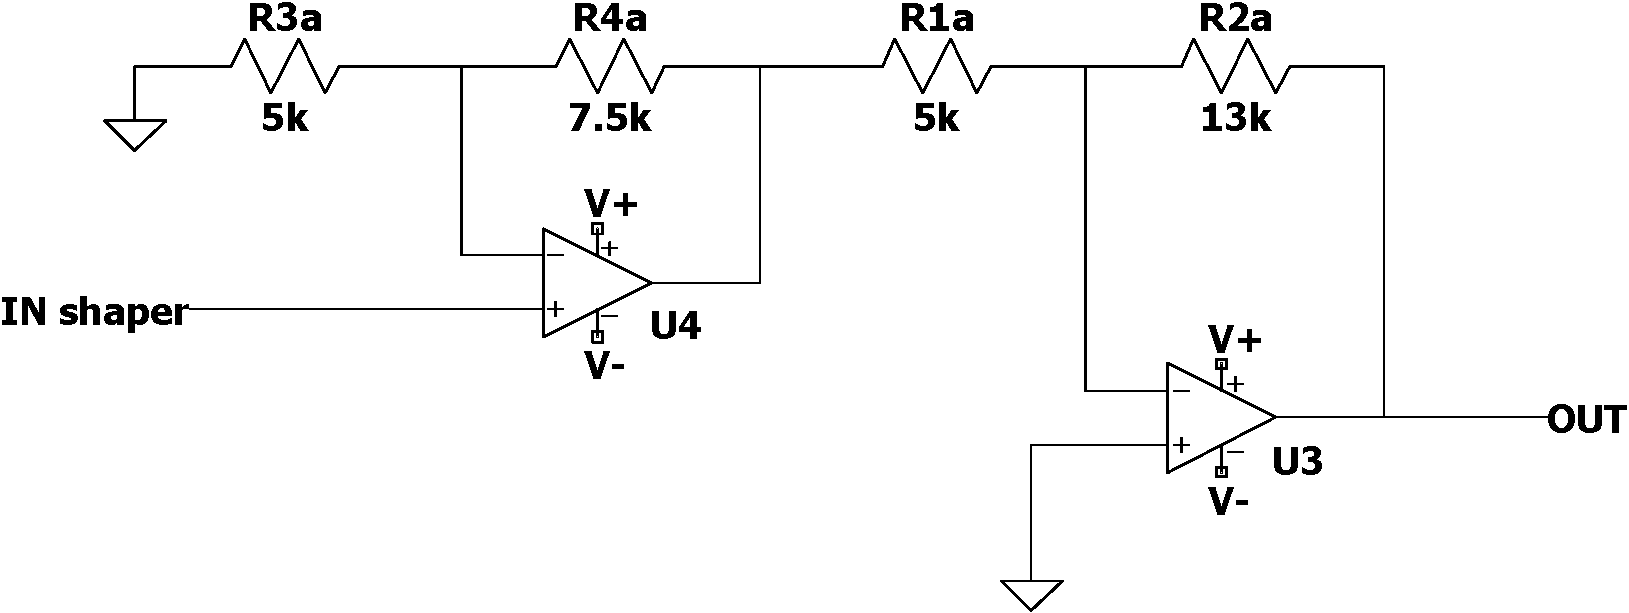
\includegraphics[scale=0.26, angle=0]{catena.pdf}
        \setlength{\belowcaptionskip}{-20pt}
        \caption{circuito amplificatore invertente}
        \label{fig:invertnete}
    \end{figure}
\end{center}

Da semplici considerazioni si trova che la funzione di trasferimento è costante rispetto alla frequenza e data dal

\begin{equation}
    \label{eqn:ampinv_trasf}
    H = - \frac{R_{2a}}{R_{1a}} \left( \frac{R_{4a}}{R_{3a}} + 1 \right)
\end{equation}

Innanzitutto si è predisposta la corretta amplificazione, per poter visualizzare segnali dell'ordine di qualche volt immettendo
nel circuito impulsi della durata di qualche unità di $\mu s$: si deve dunque considerare la quantità di carica $Q_{in}$ 
scegliendo un impulso di durata $10 \mu s$ in ingresso, misurare l'uscita dell'apparato preamplificatore + shaper $V_{sh}$ 
e si calcola l'opportuno apparato resistivo in modo da generare in uscita un segnale di approssimativamente 2 V, cioè imporre, usando
la \ref{eqn:ampinv_trasf}, H = 2 V/$V_{sh}$, dove $V_{sh}$ corrisponde al picco in uscita dal formatore.

Variando poi la durata dell'impulso di $V_{in}$ e quindi la carica $Q_{in}$ è verificata la relazione lineare che ancora
intercorre con il $V_{out}$ della catena completa.

Introducendo poi segnali sinusoidali in ingresso di frequenza variabile si è effettuato un grafico di Bode per verificare la risposta
in frequenza della catena elettronica. Combinando quindi le funzioni di trasferimento del circuito preamplificatore 
\ref{eqn:preamp_trasf}, dello shaper compensato \ref{eqn:shapercomp_trasf} e dell'amplificatore di strumentazione 
\ref{eqn:ampinv_trasf}, si ottiene la funzione di trasferimento totale.

\begin{multline}
    \label{eqn:catena_trasf}
    |H(\omega)| = \frac{R_{pre}}{R_{in}} \frac{1}{\sqrt{1+\omega^2\tau_{pre}^2}} \cdot \\
    \cdot \frac{R_{sh}^2 + \omega^2 R_{pz}^2 \tau_{sh}^2}{(R_{sh}+R_{pz})^2 + \omega^2 R_{pz}^2 \tau_{sh}^2} \cdot \\
    \cdot \frac{R_{2a}}{R_{1a}} \left( \frac{R_{4a}}{R_{3a}} + 1 \right)
\end{multline}

\subsection{Discussione dati}

Utilizzando quindi il circuito fin qui costruito e iniettando la $V_{in}$ di cui sopra si trova $V_{sh} = (-282 \pm 5) mV$, pertanto
$H_{th} \approx 7$. Si può dunque scegliere le resistenze di conseguenza, in particolare:

\begin{align*}
    R_{1a} = (15.003 \pm 0.007) k\Omega \quad \sigma_{\%} = 0.05\% \\
    R_{2a} = (32.57 \pm 0.01) k\Omega \quad \sigma_{\%} = 0.04\% \\
    R_{1a} = (14.999 \pm 0.007) k\Omega \quad \sigma_{\%} = 0.05\% \\
    R_{1a} = (32.60 \pm 0.01) k\Omega \quad \sigma_{\%} = 0.04\% \\
\end{align*}

da cui $H_{sper}=-6.88$. Realizzato dunque il circuito si è proceduto con l'acquisizione di $V_{out}$ al variare dell'impulso in
ingresso, di cui si riportano di seguito dati e fit lineare.

\begin{center}
    \begin{figure}[H]
        \centering
        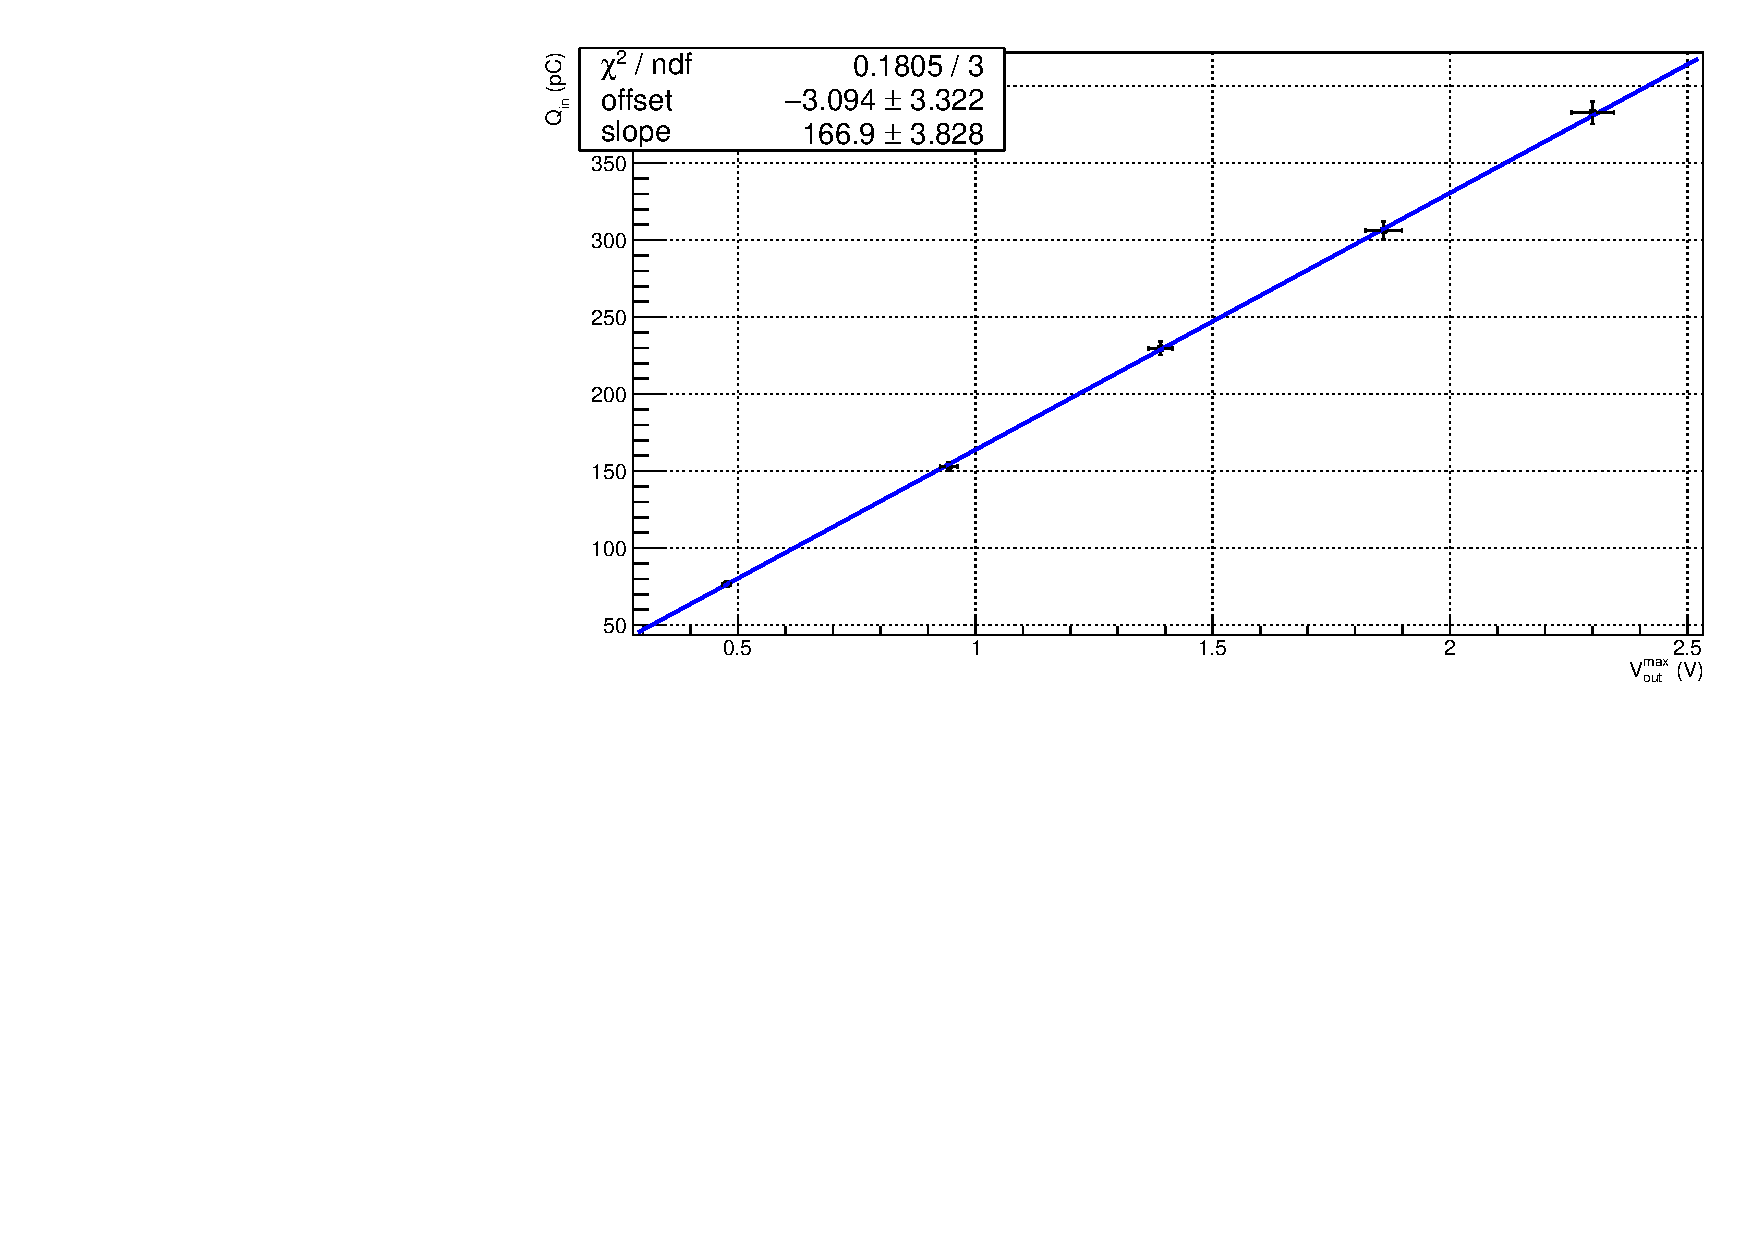
\includegraphics[scale=0.4, angle=0]{fitcatena.pdf}
        \setlength{\belowcaptionskip}{-20pt}
        \caption{Relazione lineare tra carica iniettata e uscita della catena}
        \label{fig:catenaQvsV}
    \end{figure}
\end{center}

\begin{center}
    \begin{figure}[H]
        \centering
        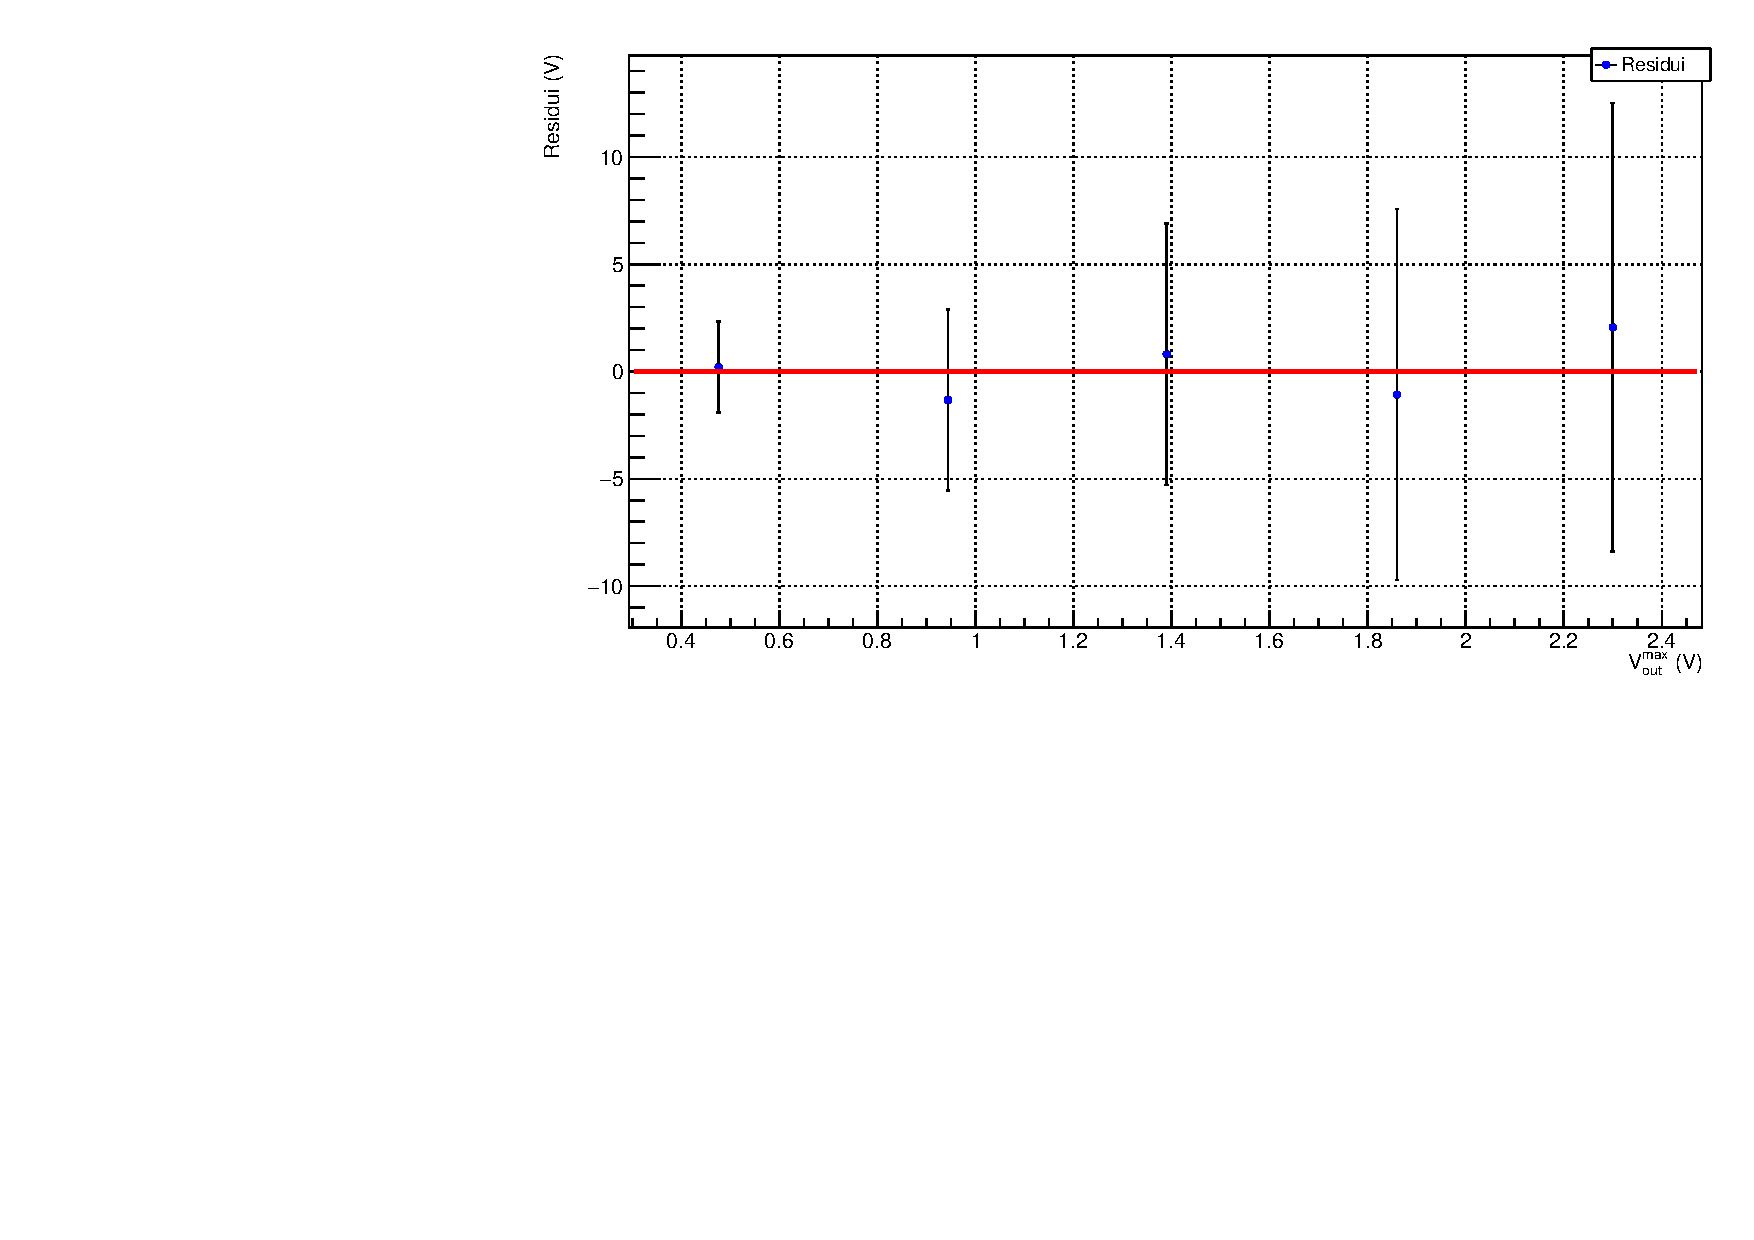
\includegraphics[scale=0.4, angle=0]{residuicatena.pdf}
        \setlength{\belowcaptionskip}{-20pt}
        \caption{Grafico dei residui della relazione tra $Q_{in}$ e $V_{out}$}
        \label{fig:catenaQvsV_res}
    \end{figure}
\end{center}

\begin{table}[ht]
    \centering
    \begin{tabular}{ccccc}
        \toprule
        $\sigma_{y, post}$    &$\chi^{(2)}$    &$\lambda_{\chi}$   &$\rho$ &t   \\
        \midrule
        1.6 pC                &0.18            &1.15               &0.99994&167.63\\
        \bottomrule
    \end{tabular}
    \caption{parametri di verifica della bontà del fit}
\end{table}

Si osserva che i parametri di bontà del fit sono buoni, a testimonianza di una ben verificata relazione

Successivamente si presenta il grafico di Bode della catena, in cui sono raffigurati i dati sperimentali, i dati simulati
su LTspice e il modello teorico espresso dalla \ref{eqn:catena_trasf}.



\begin{center}
    \begin{figure}[H]
        \centering
        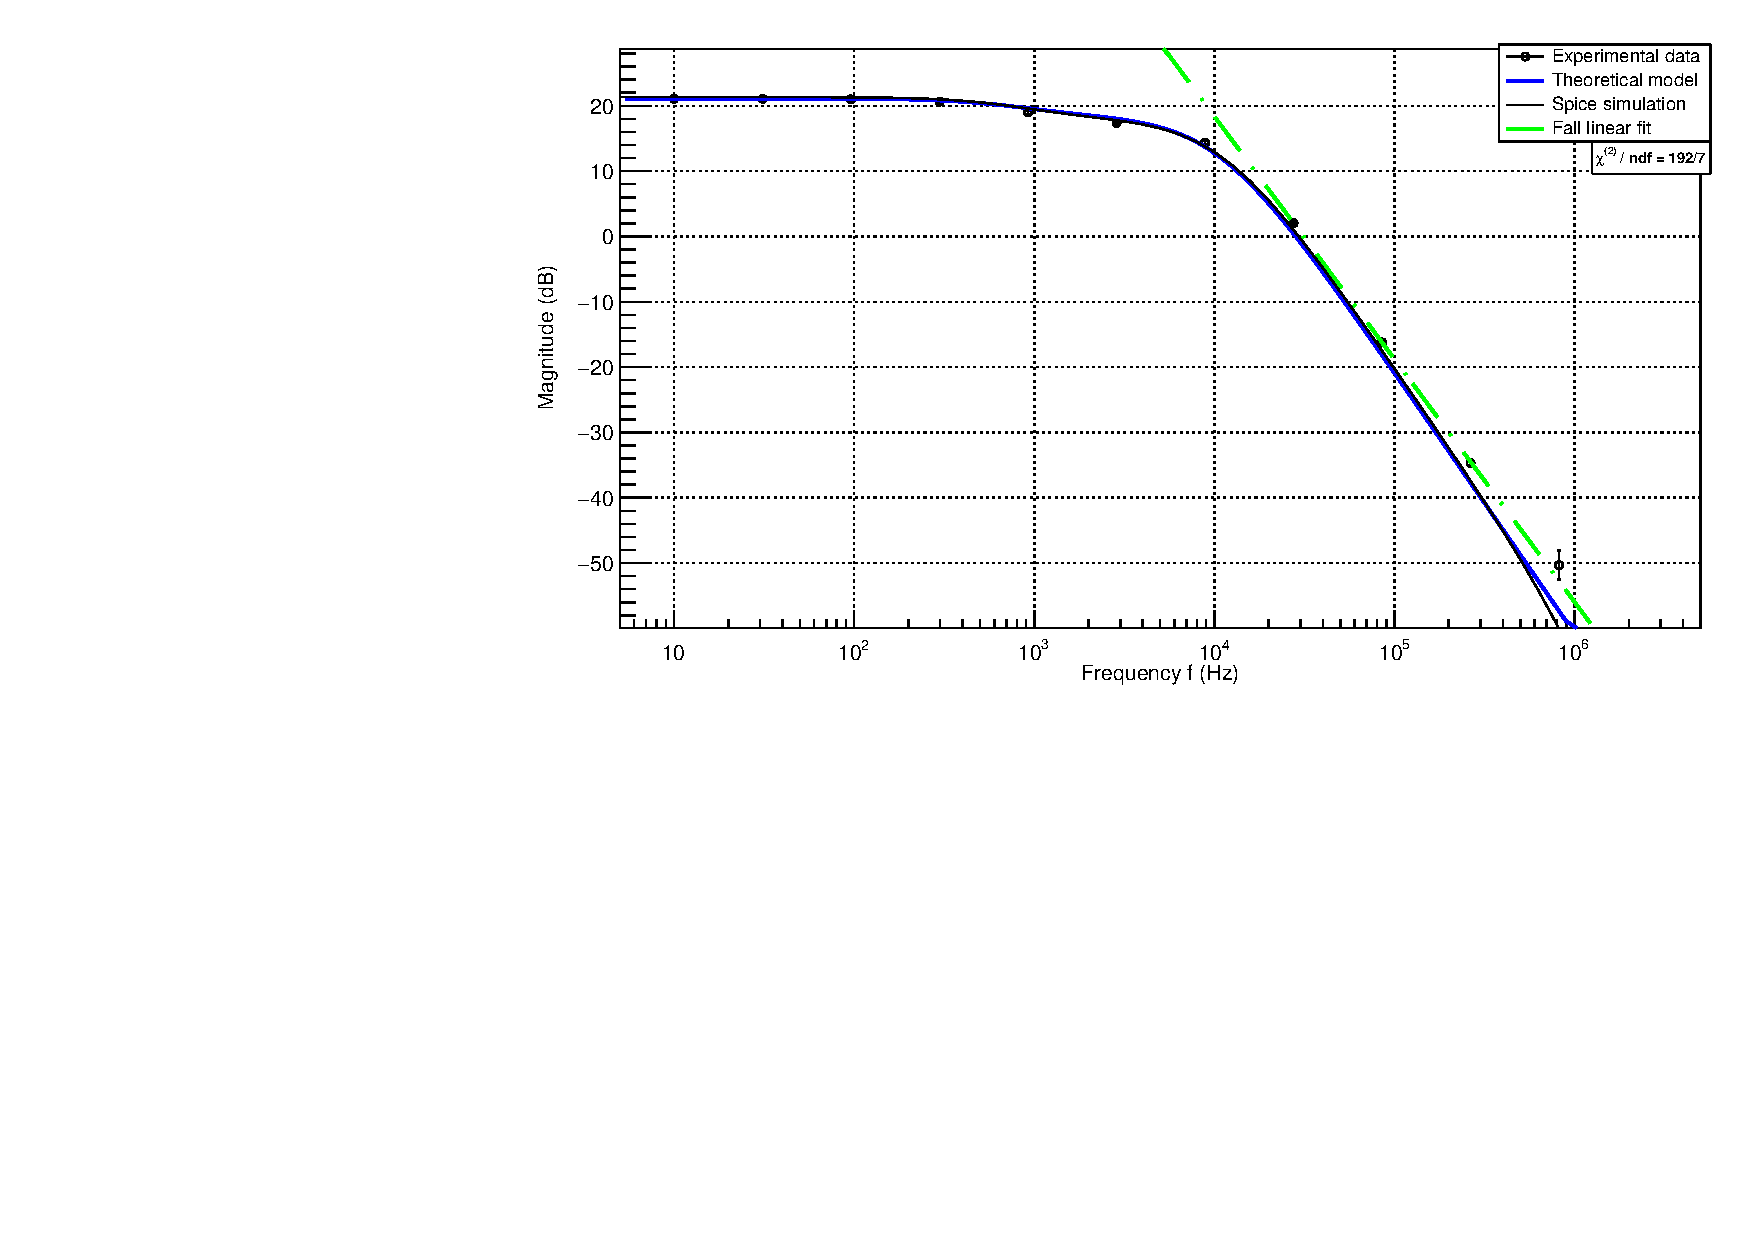
\includegraphics[scale=0.4, angle=0]{bodecatena.pdf}
        \setlength{\belowcaptionskip}{-20pt}
        \caption{grafico di Bode della risposta in frequenza della catena elettronica}
        \label{fig:catenaBODE}
    \end{figure}
\end{center}

\begin{center}
    \begin{figure}[H]
        \centering
        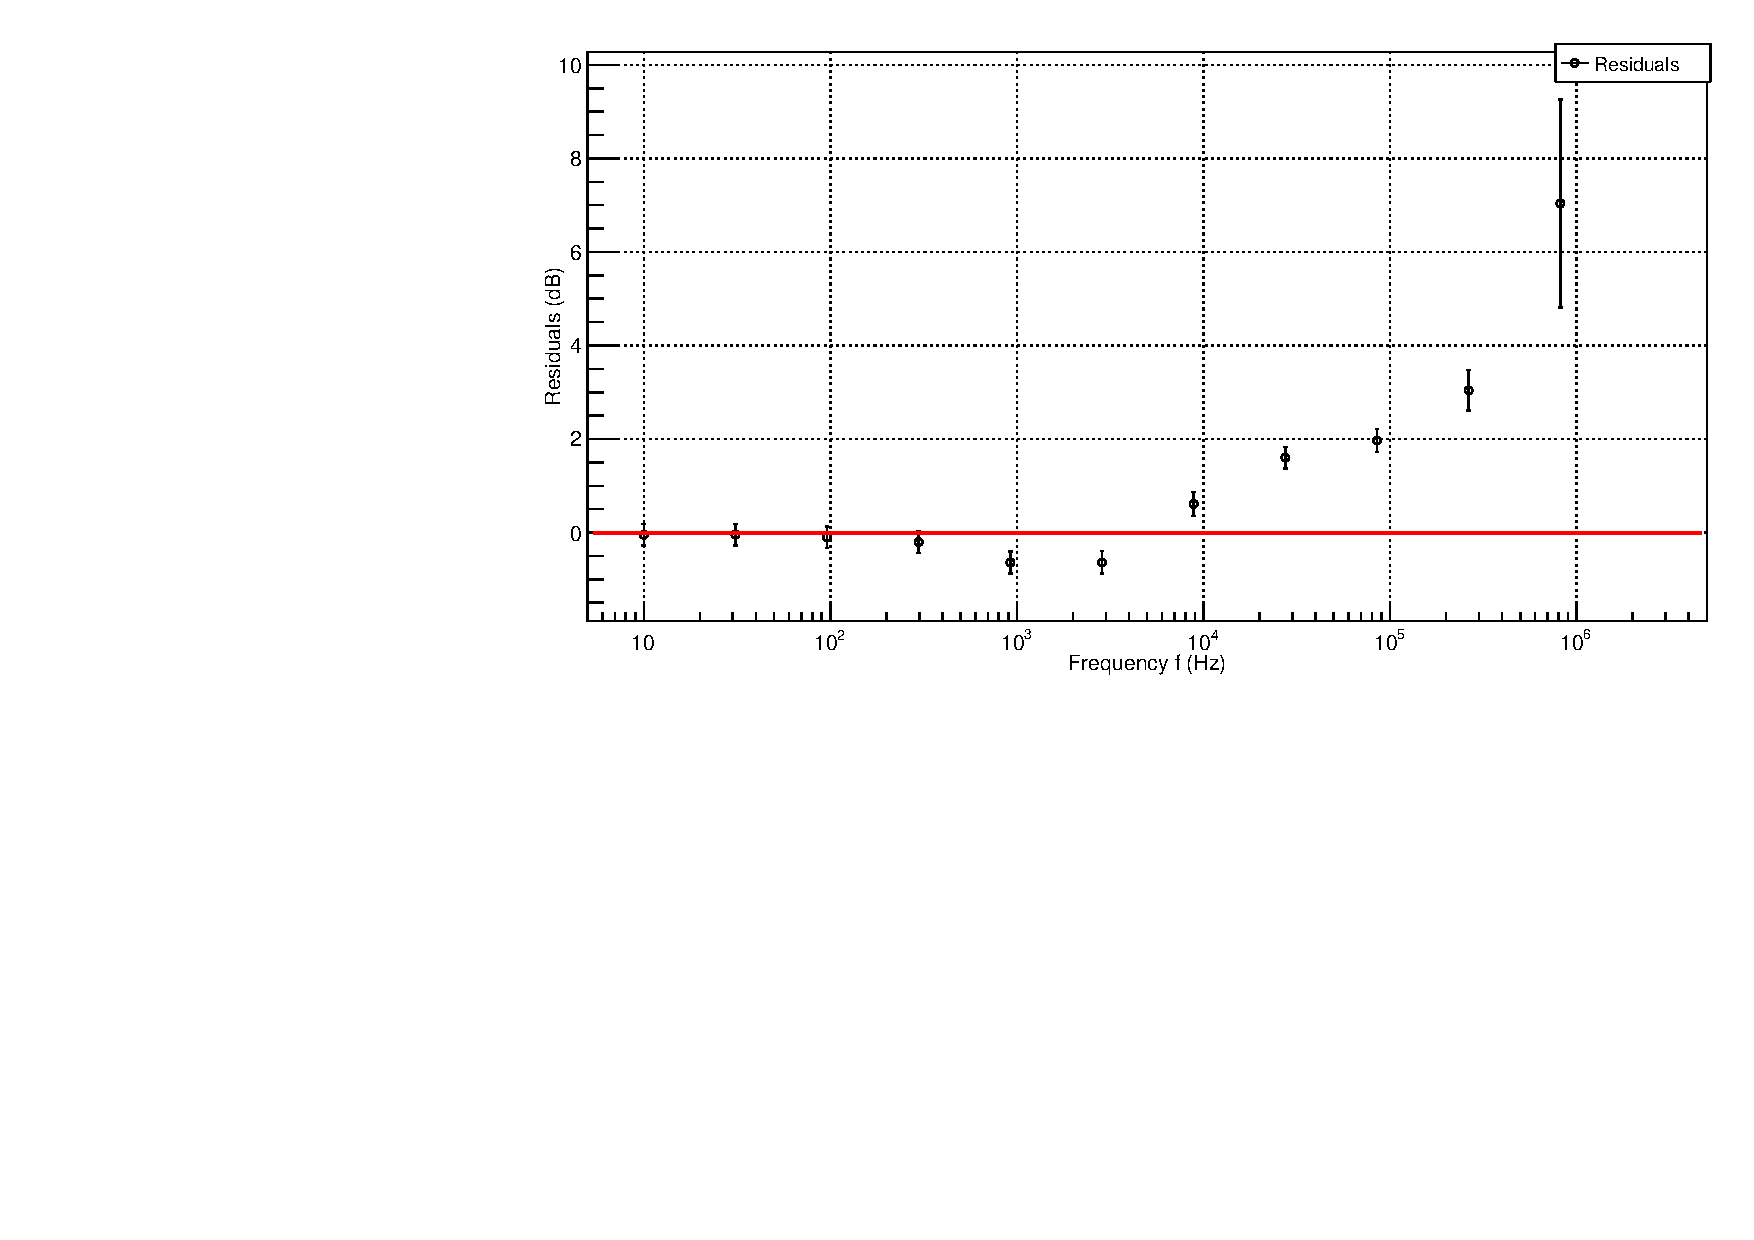
\includegraphics[scale=0.4, angle=0]{bodecatenaresidui.pdf}
        \setlength{\belowcaptionskip}{-20pt}
        \caption{grafico dei residui tra dati sperimentali e modello}
        \label{fig:catenaBODE_res}
    \end{figure}
\end{center}

Si può osservare una forte incompatibilità dei dati con il modello teorico: il valore
di $\chi^{(2)}$ risulta assolutamente incompatibile con il suo valore di aspettazione.
Come si può osservare nel grafico dei residui, le problematiche sono sulle alte frequenze:
questo fenomeno, alla luce dei problemi su preamplificatore e shaper in cui la curva teorica
aveva problemi sulle alte frequenze, era preventivabile: infatti la funzione di trasferimento
della catena completa altro non è che il prodotto delle funzioni delle sue singole parti, quindi 
tali problematiche si amplificano.

Si è infine effettuato un fit della discesa per verificare che la pendenza sia compatibile con -40 dB/decade.

\begin{table}[ht]
    \centering
    \begin{tabular}{rcccc}
        \toprule
                &\multicolumn{2}{c}{a$\pm \sigma_a$} &\multicolumn{2}{c}{b$\pm \sigma_b$}\\
                &\multicolumn{2}{c}{(dB)}  &\multicolumn{2}{c}{(dB/decade)}\\
        \midrule
        discesa &\multicolumn{2}{c}{167$\pm$2}&\multicolumn{2}{c}{-37.2$\pm$0.5}\\
        \bottomrule
    \end{tabular}
    \caption{parametri di interpolazione lineare della discesa}
\end{table}


\begin{center}
    \begin{figure}[H]
        \centering
        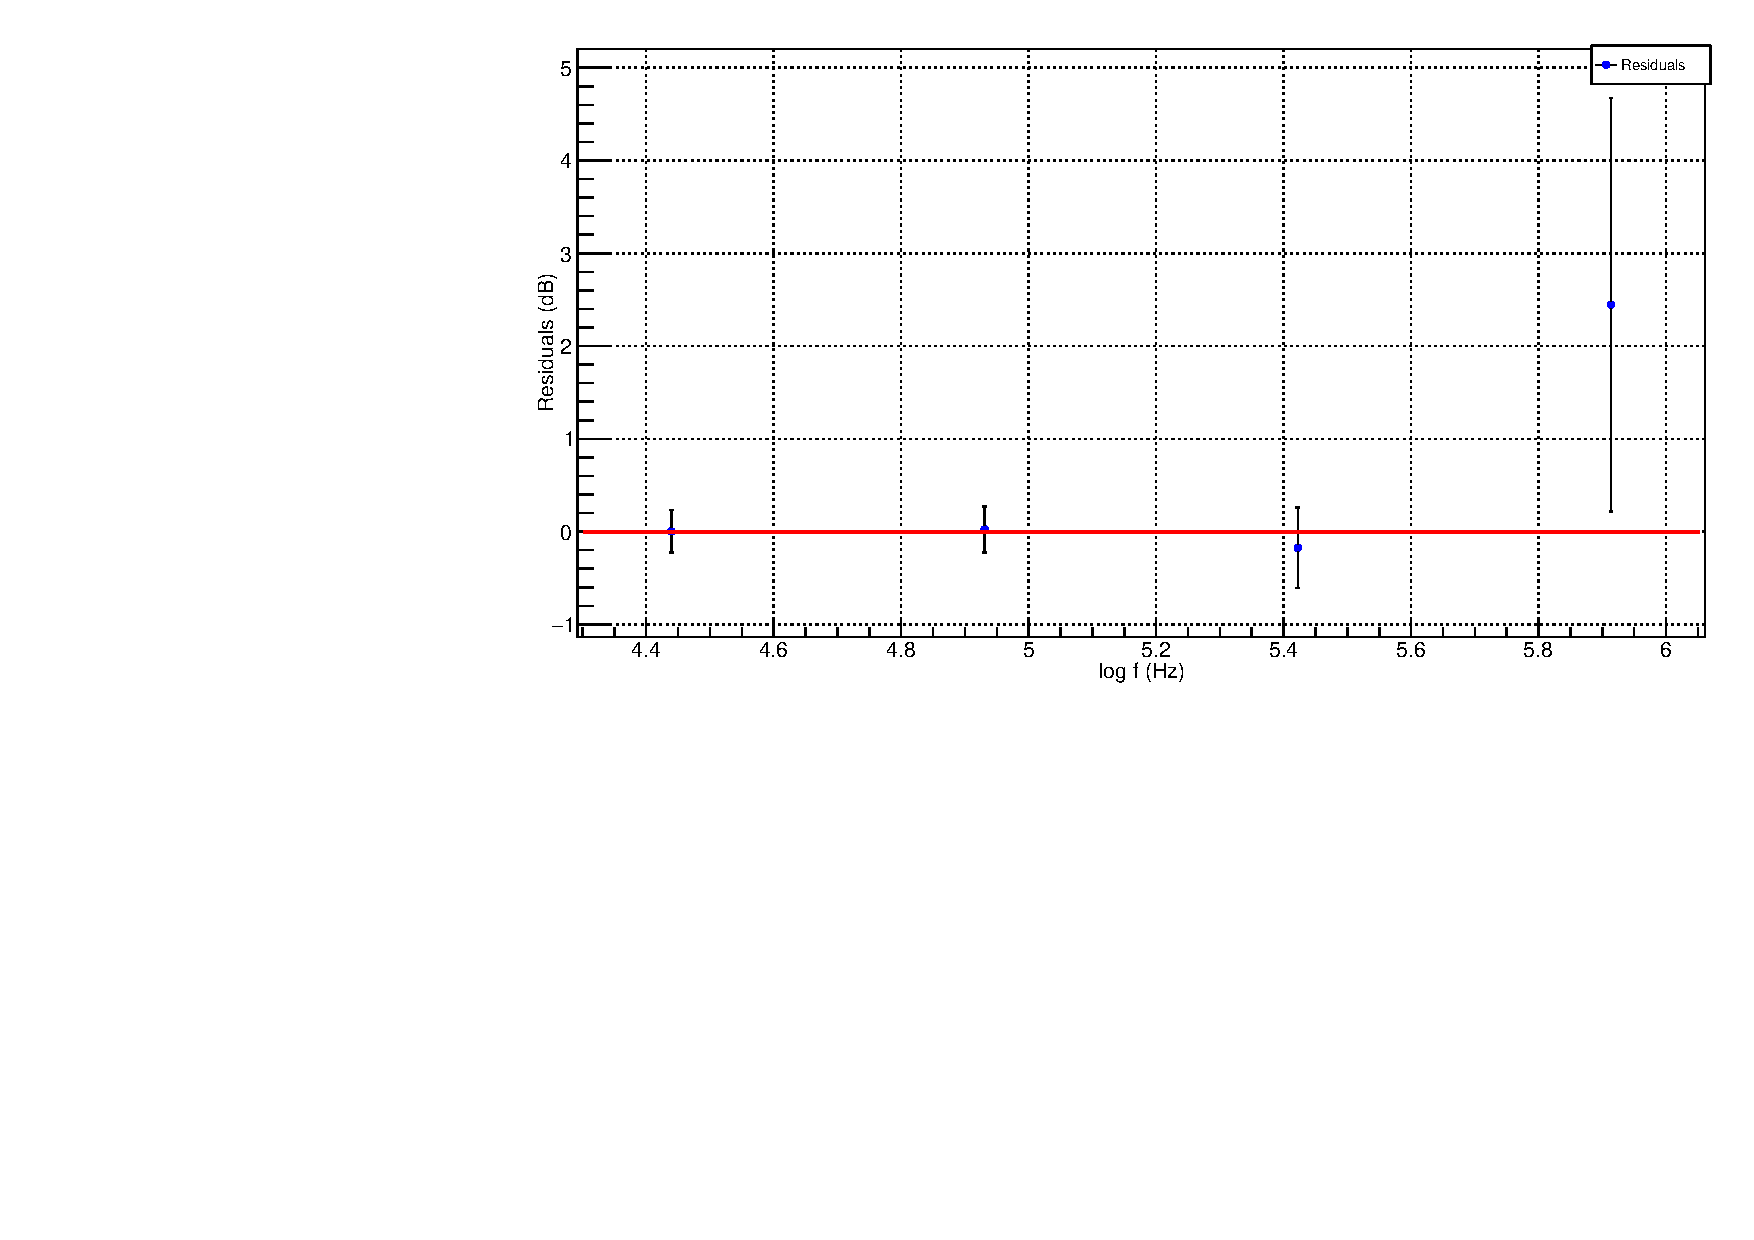
\includegraphics[scale=0.375, angle=0]{residuicatenadiscesa.pdf}
        \setlength{\belowcaptionskip}{-20pt}
        \caption{grafico dei residui del fit della discesa della catena}
        \label{fig:residuicatenadiscesa}
    \end{figure}
\end{center}

\begin{table}[ht]
    \centering
    \begin{tabular}{ccccc}
        \toprule
        $\sigma_{y, post}$    &$\chi^{(2)}$    &$\lambda_{\chi}$   &$\rho$  &t   \\
        \midrule
        1.7 dB                &1.38           &1.12              &-0.9993&-37.85\\
        \bottomrule
    \end{tabular}
    \caption{parametri di verifica della bontà del fit}
\end{table}

Si nota ancora una volta che la pendenza non è compatibile con il valore atteso ($\lambda \approx 5.6$). Il fatto, alla luce delle analisi precedenti,
non stupisce: i problemi incontrati nelle precedenti sezioni si ripercuotono fin qui.

\section{Acquisizione forme d'onda con Arduino}

Ora la catena elettronica restituisce un segnale correttamente processato e amplificato, adatto alla rivelazione da parte di una scheda Arduino Due. Prima di iniziare
l'acquisizione delle forme d'onda restituite dal circuito, occorre comprendere la taratura della scheda per poi gestire i dati sperimentali. Si effettuano dunque delle 
acquisizioni preliminari al fine di realizzare una calibrazione orizzontale (sui tempi) e una verticale (sulle tensioni).

In particolare per la calibrazione orizzontale si sono utilizzate onde sinusoidali di diversa frequenza (e dunque periodo), confrontando
il periodo T con il conteggio dei punti nell'acquisizione secondo la formula $T = a + b \cdot ch$, dove ch rappresenta il periodo in 
counts stimato attraverso un algoritmo che individua gli zeri nella forma sinusoidale traslata in modo da essere simmetrica rispetto all'asse
delle ascisse. Per brevità si riporta, per entrambe le calibrazioni, un solo set di dati.

\begin{center}
    \begin{figure}[H]
        \centering
        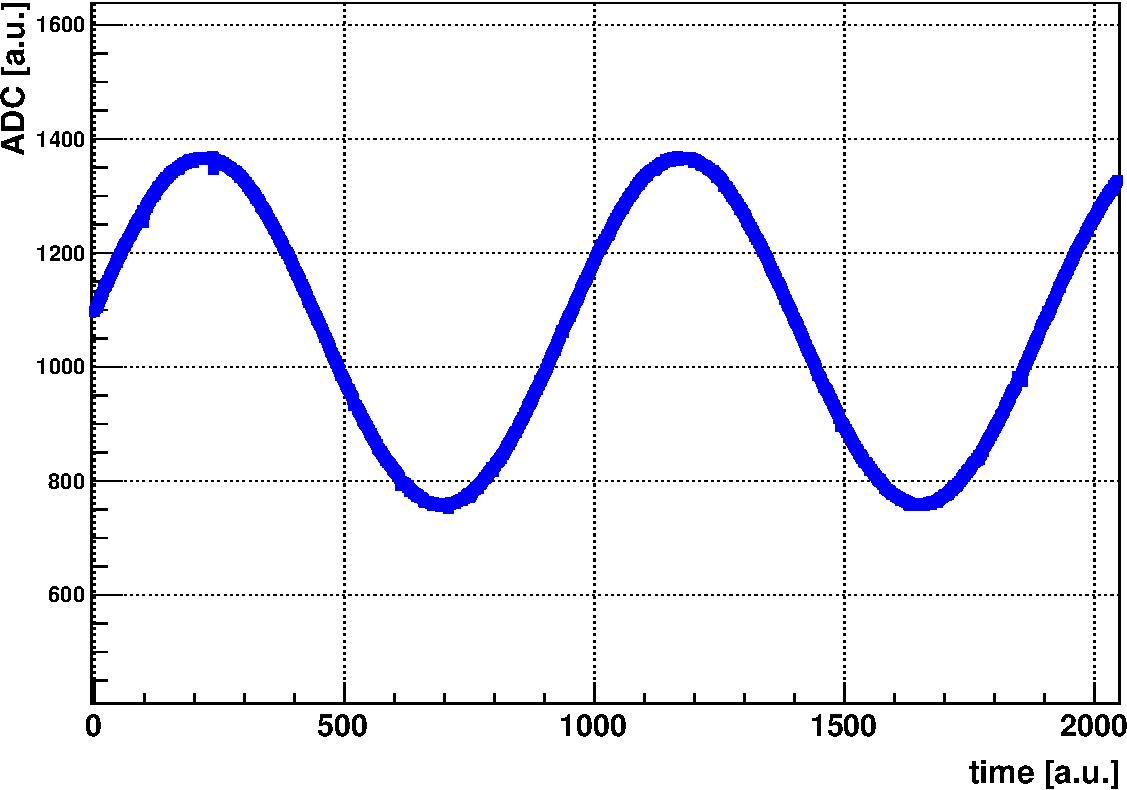
\includegraphics[scale=0.4, angle=0]{4_1.pdf}
        \setlength{\belowcaptionskip}{-20pt}
        \caption{acquisizione forma sinusoidale per frequenza 1 kHz}
        \label{fig:period_counts}
    \end{figure}
\end{center}

\begin{center}
    \begin{figure}[H]
        \centering
        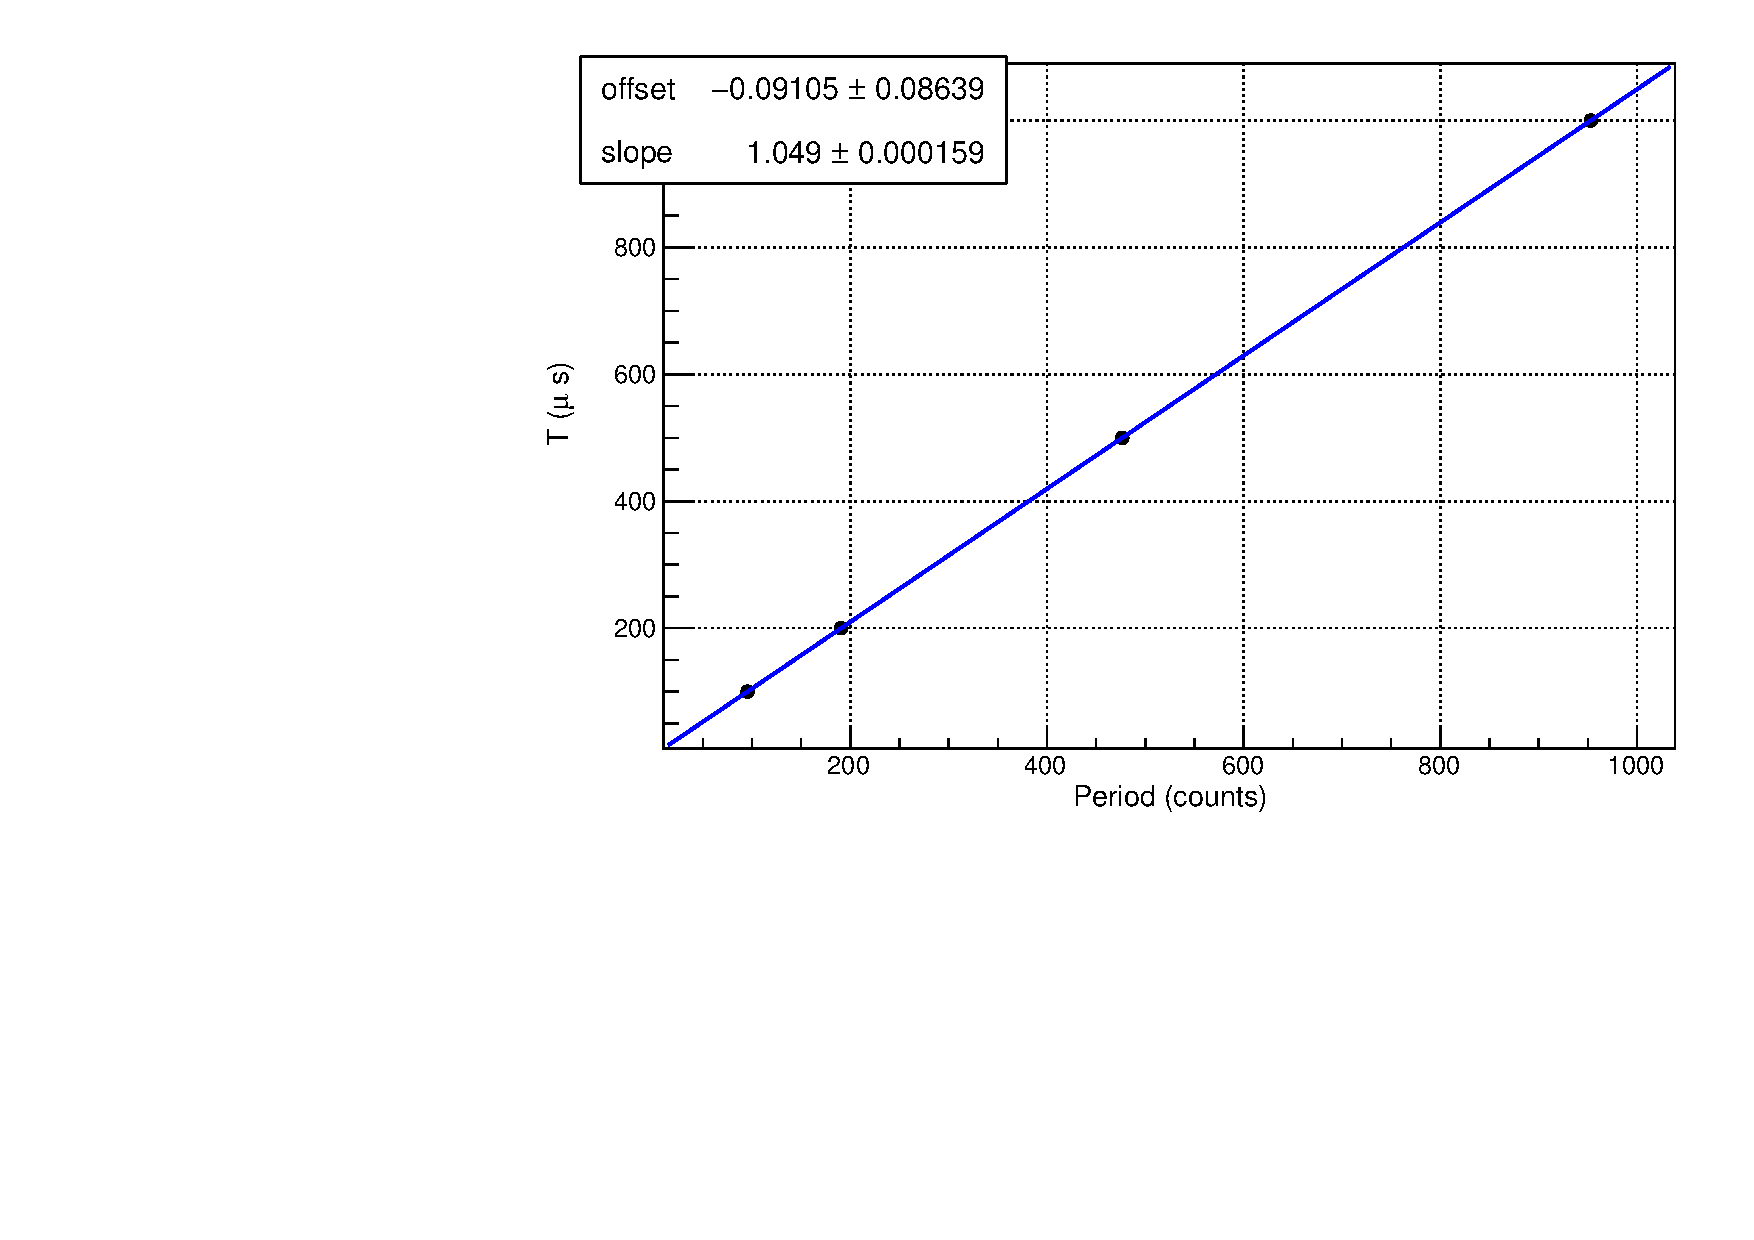
\includegraphics[scale=0.4, angle=0]{calibtempi.pdf}
        \setlength{\belowcaptionskip}{-20pt}
        \caption{calibrazione temporale}
        \label{fig:calibtempi}
    \end{figure}
\end{center}

Ne si ricava che il software acquisisce un punto in ogni intervallo pari alla slope b, ossia ogni $(1.0490 \pm 0.0002)\mu $s.
Inoltre, come atteso il valore di offset risulta compatibile con lo 0.

Per la calibrazione verticale sulle tensioni si sono immesse nel circuito onde quadrate tra 0 e una tensione di altezza variabile, 
per poi effettuare nuovamente un fit lineare del tipo $V = a + b \cdot ch$, dove ch stavolta indica l'altezza dei plateau della tensione 
in conteggi: il parametro $b$ fornirà il fattore di conversione mV/counts, mentre $a$ mostra l'offset aggiunto dalla scheda arduino alla tensione effettiva.

\begin{center}
    \begin{figure}[H]
        \centering
        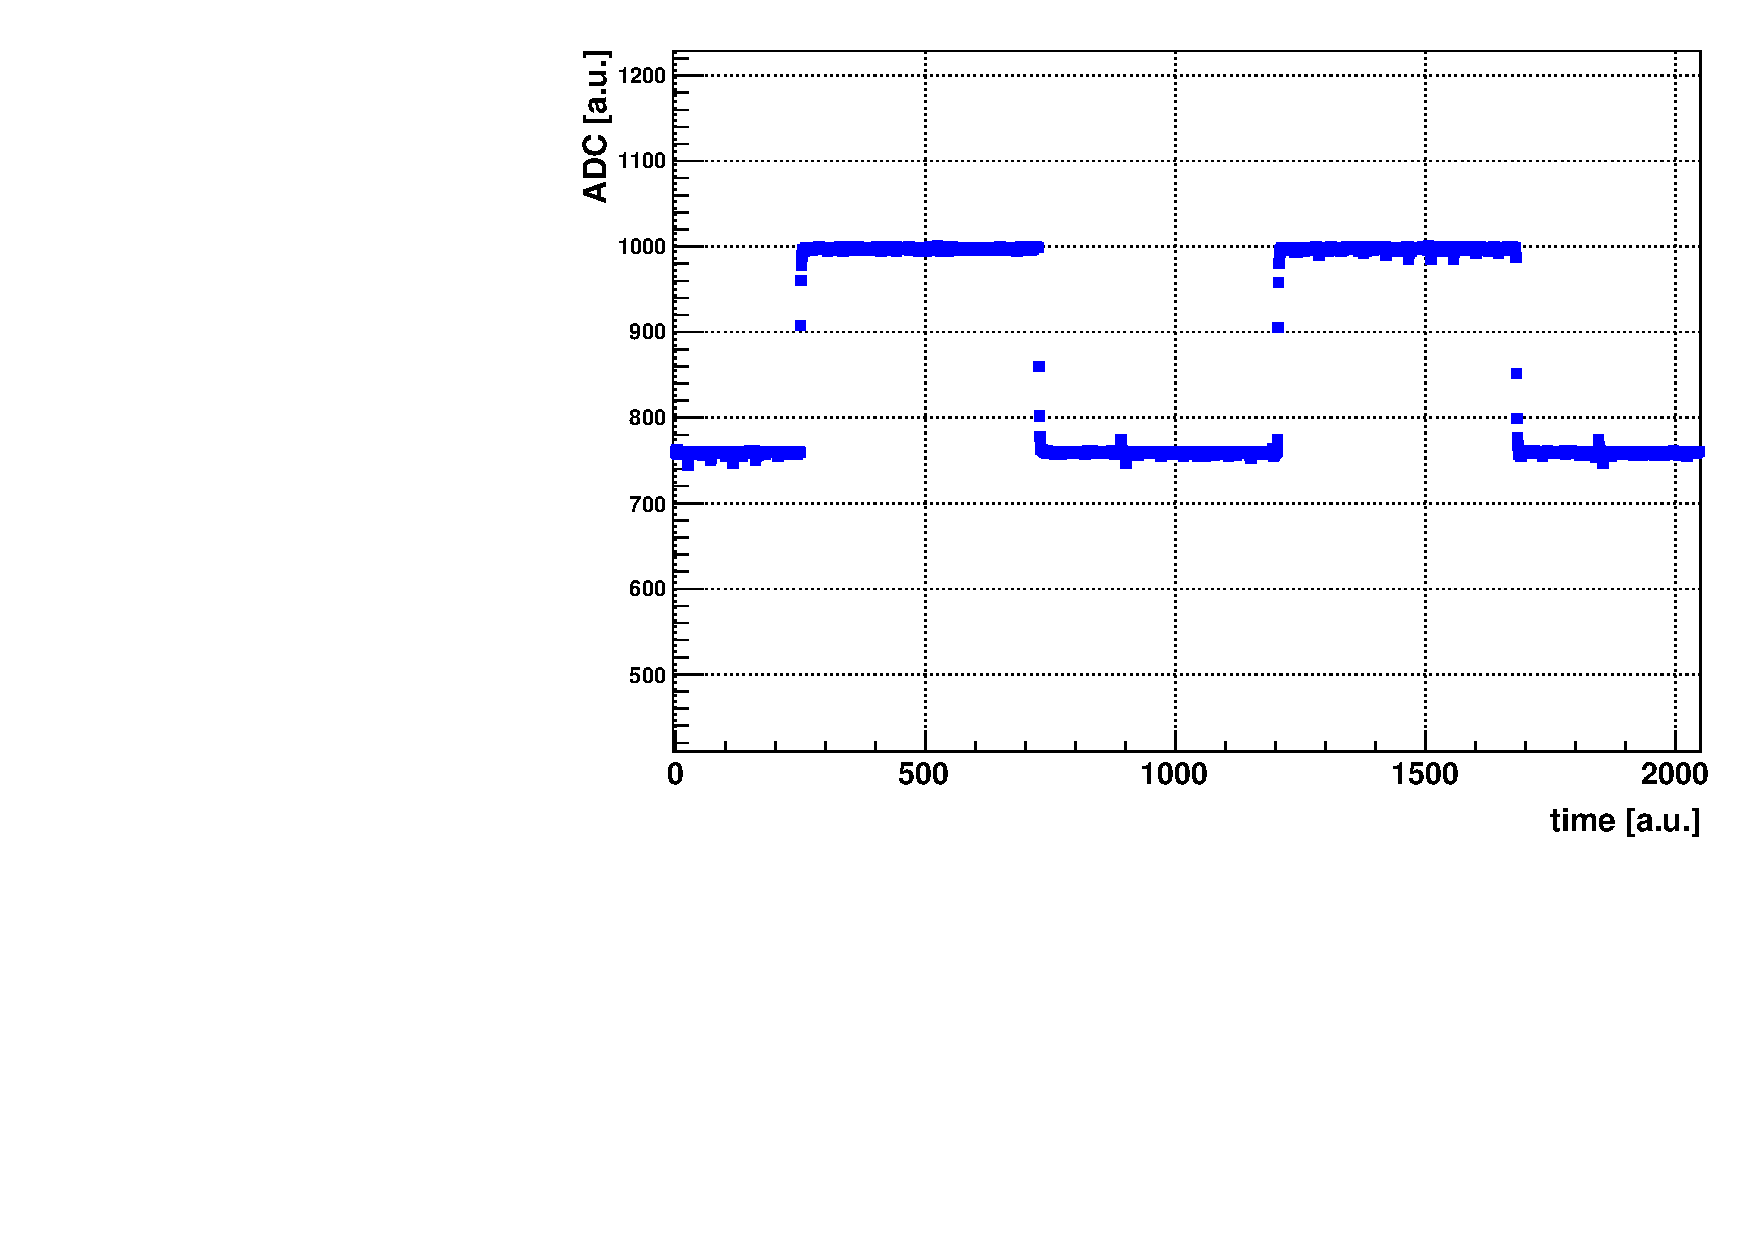
\includegraphics[scale=0.4, angle=0]{4_2.pdf}
        \setlength{\belowcaptionskip}{-20pt}
        \caption{acquisizione onda quadrata per tensione 200 mV}
        \label{fig:voltage_counts}
    \end{figure}
\end{center}

\begin{center}
    \begin{figure}[H]
        \centering
        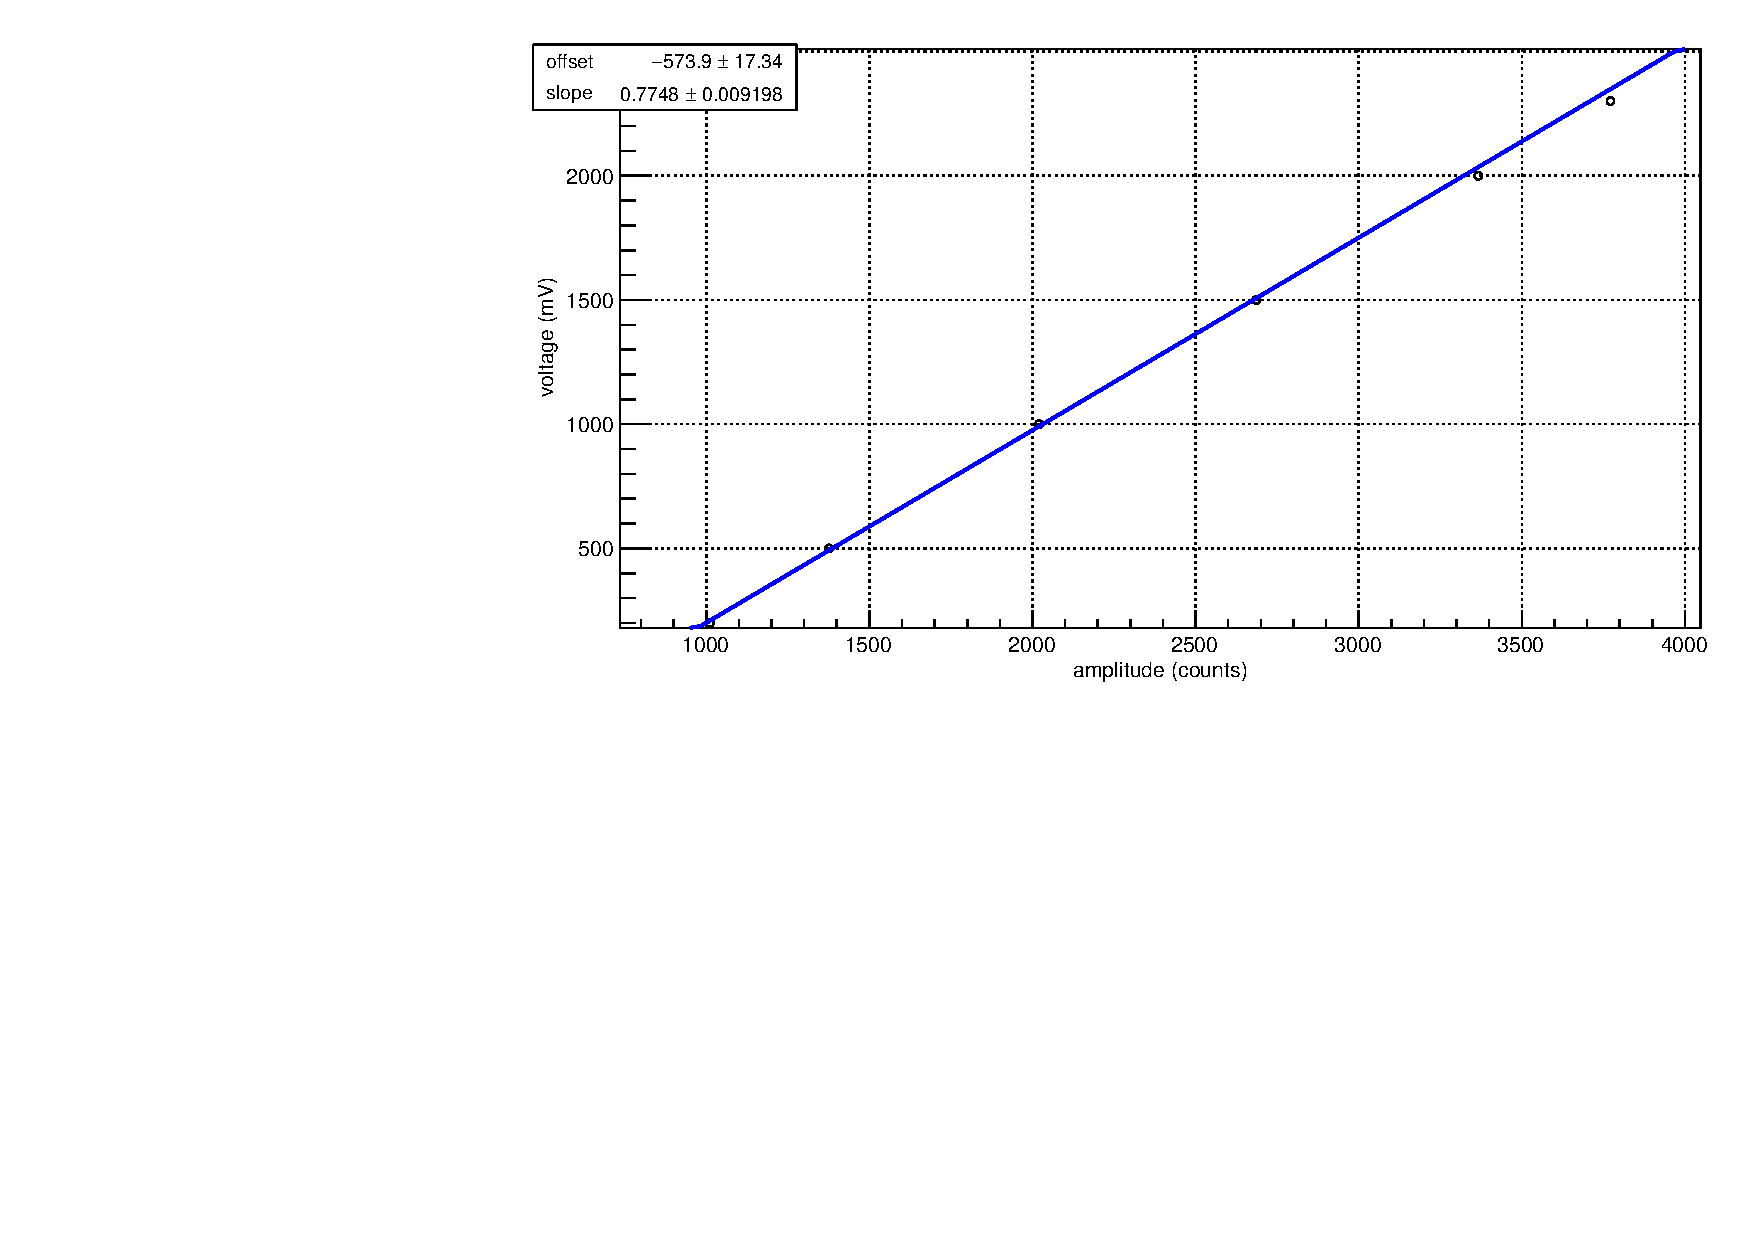
\includegraphics[scale=0.4, angle=0]{calibverticale.pdf}
        \setlength{\belowcaptionskip}{-20pt}
        \caption{calibrazione verticale}
        \label{fig:calibverticale}
    \end{figure}
\end{center}

Il valore acquisito da Arduino dovrà quindi essere moltiplicato per la slope ($0.775 \pm 0.009)$mV/counts
e traslato dell'offset ($-574 \pm 17$) mV.

L'algoritmo utilizzato in questo caso individua i punti nel plateau superiore e in quello 
inferiore, e effettua di tali punti la media in modo iterato, escludendo di volta in volta i punti che si discostano
dalla media "provvisoria" per più di $3\sigma$.



Effettuata dunque la calibrazione, si è acquisita la forma d'onda in uscita dalla catena elettronica completa con in input il solito
impulso di tensione, partendo da una durata di $10 \mu $s e diminuendola via via di un'unità ad ogni nuova acquisizione.

Si riportano di seguito, per evitare risultati ripetitivi, solamente due grafici di confronto tra la forma d'onda acquisita dalla scheda e opportunamente 
convertita con i parametri ottenuti dalla
calibrazione e la simulazione ottenuta dal software LTspice; uno dei due grafici si riferisce a un impulso in ingresso di durata 10 $\mu $s, l'altro di 2 $\mu $s.
Per realizzare al meglio tale sovrapposizione grafica, si è dovuto allineare il primo picco della simulazione con quello restituito dalla scheda, poiché Arduino
presenta un delay temporale nell'acquisizione che ostacola un corretto allineamento delle due curve.


\begin{center}
    \begin{figure}[H]
        \centering
        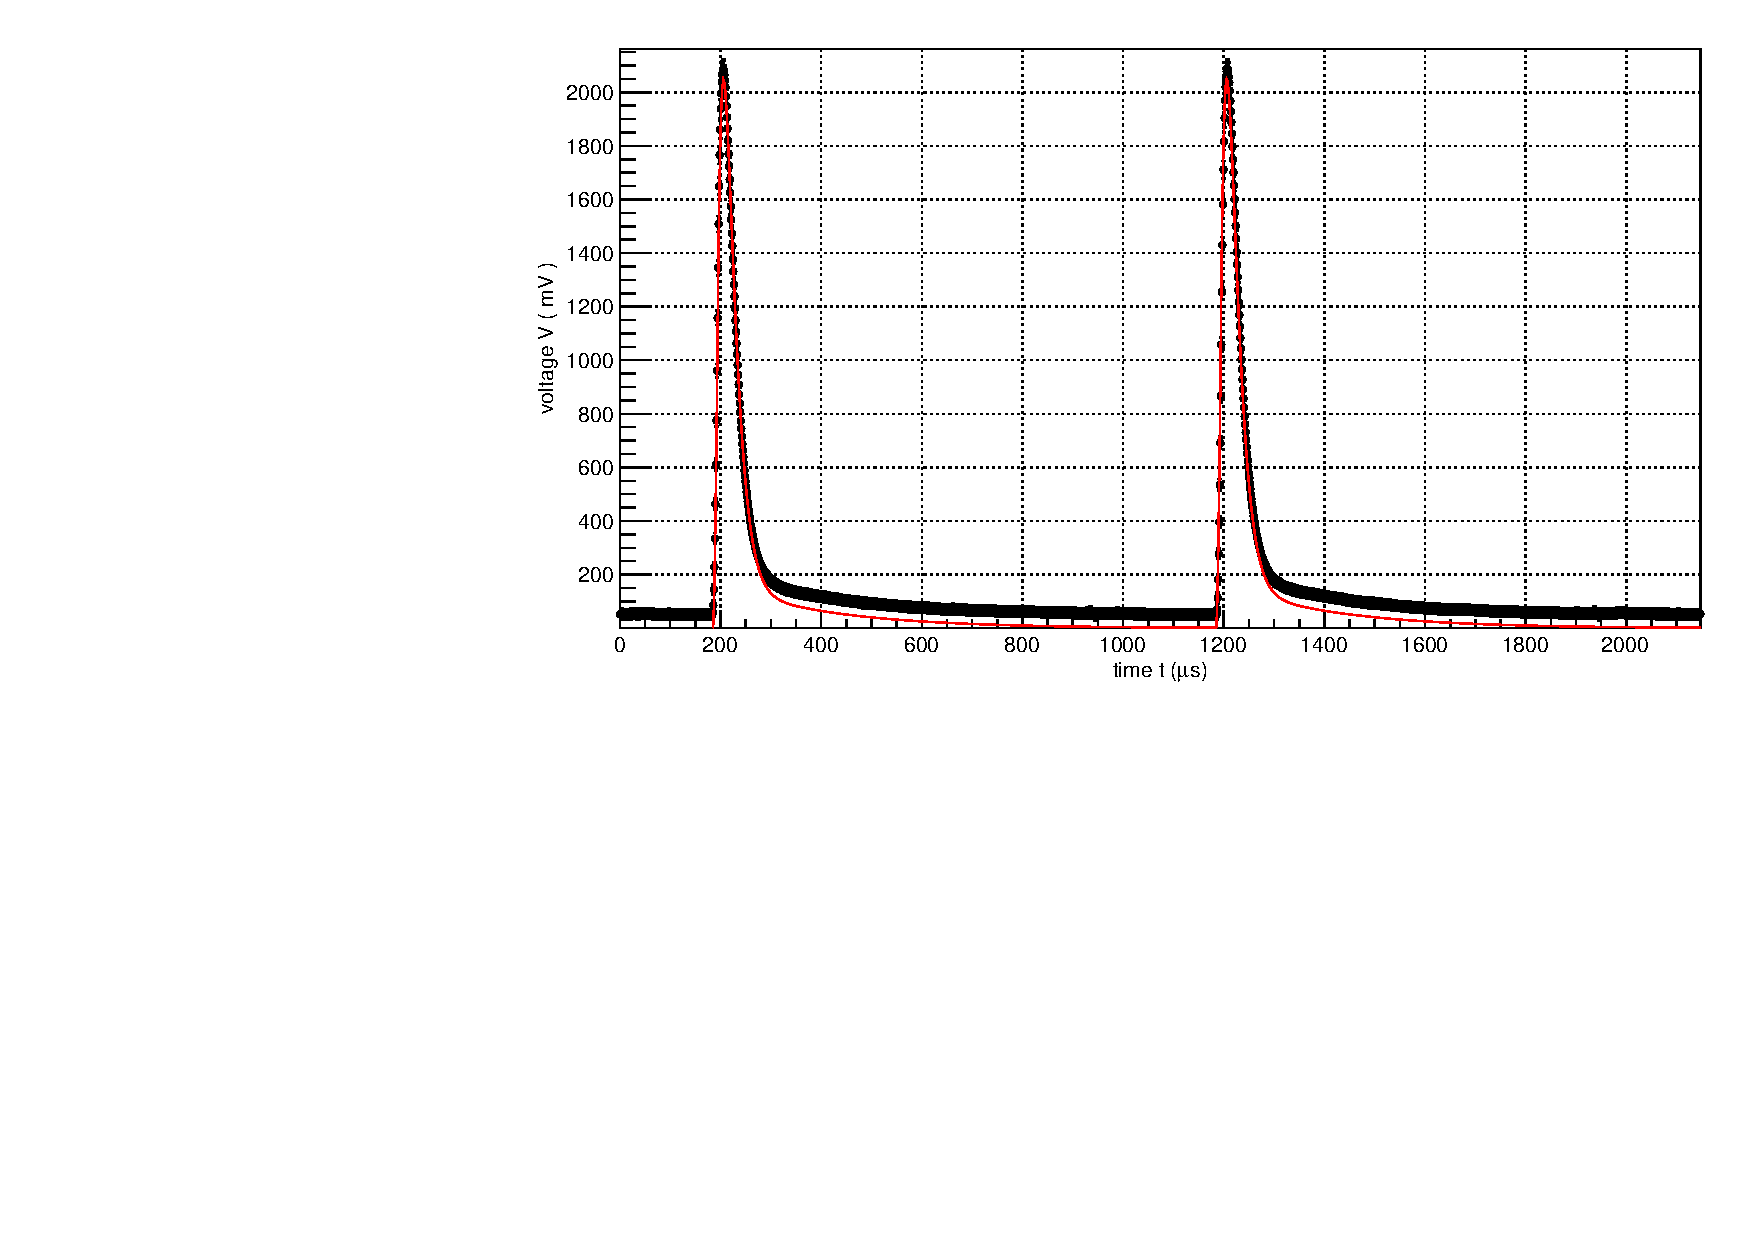
\includegraphics[scale=0.4, angle=0]{arduino10.pdf}
        \setlength{\belowcaptionskip}{-20pt}
        \caption{confronto grafico tra le due forme d'onda per $t_{pulse}=10 \mu s$}
        \label{fig:arduino10}
    \end{figure}
\end{center}

\begin{center}
    \begin{figure}[H]
        \centering
        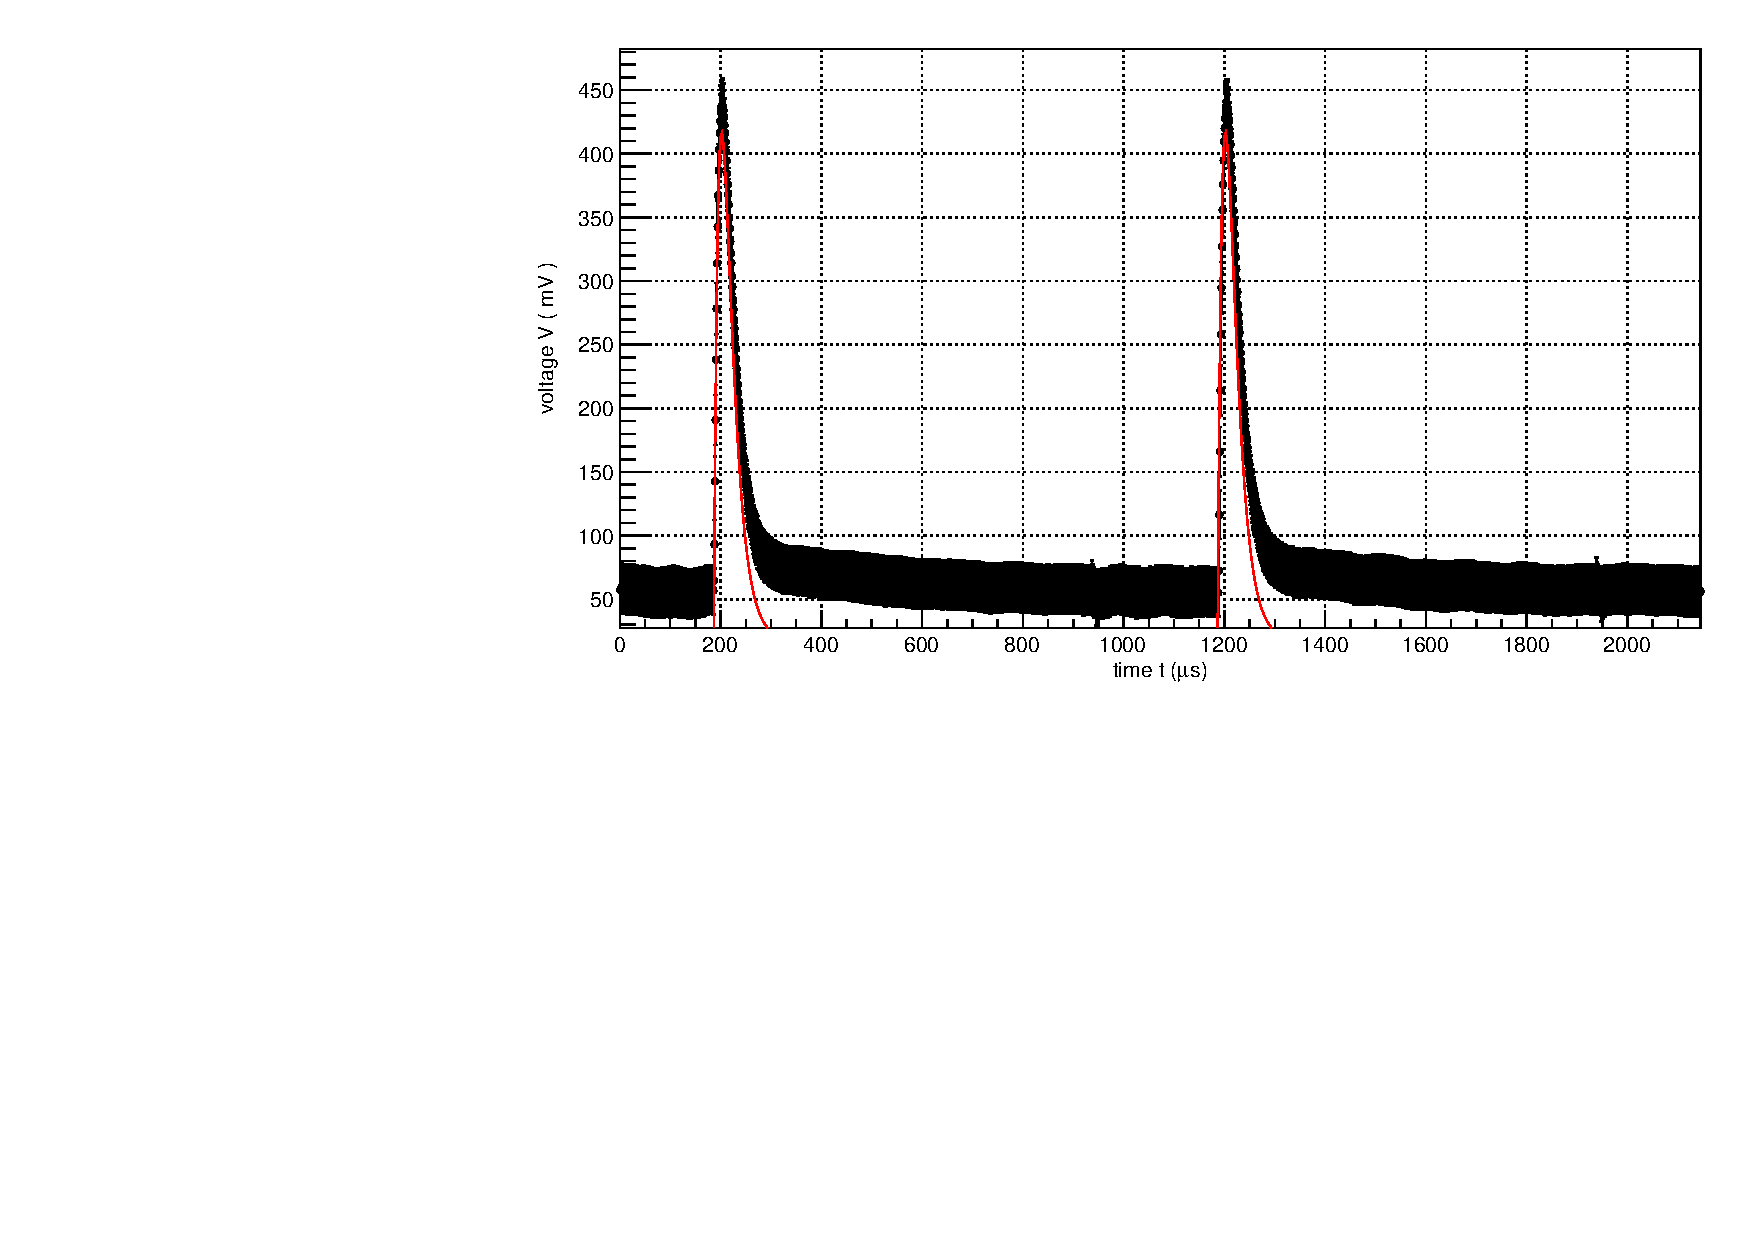
\includegraphics[scale=0.4, angle=0]{arduino2.pdf}
        \setlength{\belowcaptionskip}{-20pt}
        \caption{confronto grafico tra le due forme d'onda per $t_{pulse}=2 \mu s$}
        \label{fig:arduino2}
    \end{figure}
\end{center}


Oltre al confronto grafico, si è eseguita anche un'analisi dei picchi (due per ciascun grafico): nello specifico, poichè il campionamento risulta sufficientemente fitto, si è preso il massimo
acquisito come riferimento. Si è anche calcolata la distanza in 
$\sigma$ tra il picco simulato e acquisito, dove $\sigma$ è l'errore associato al massimo: l'errore sui punti della simulazione
è considerato trascurabile, motivo per cui la distanza è valutata solamente in unità di errore dei dati sperimentali.
Inoltre, si riporta un controllo asintotico della distanza in forma di compatibilità tra le code delle due forme d'onda, per verificare che queste 
si adagino correttamente allo zero: in particolare si è scelto un intervallo di tempo appena precedente all'innalzamento del secondo picco e si è eseguita la media
pesata tra i valori di tensione associati agli estremi di tale intervallo, con errore fornito dall'errore della media pesata. Nel caso della forma simulata, priva di 
errore sui punti, si è svolta invece una media semplice attribuendo l'errore della media.

Già da un confronto visivo immediato si intuisce la presenza di un discreto offset tra la simulazione e la forma convertita da Arduino, che si ripercuote
anche nella compatibilità tra le coppie di picchi rispettive e nel controllo dello stato asintotico, in cui tale scarto risalta in modo notevole, come esposto
nel seguito.


Come anticipato, segue un confronto tra i picchi di tensione, uno tra i tempi del secondo picco (per verificare che persista la corretta periodicità),
e infine il controllo della distanza delle tensioni asintotica $V_{as}$. 

\begin{table}[H]
    \centering
    \begin{tabular}{cccc}
        \toprule
                        & Arduino & Simulazione & Compatibilità \\
        \midrule
        $V_{peak}^{(1)}$    &   \multirow{2}{*}{$2086 \pm 36$} & \multirow{2}{*}{$2046.19$} & \multirow{2}{*}{1.1 $\sigma$}\\
        (mV)\\
        $V_{peak}^{(2)}$    &   \multirow{2}{*}{$2088 \pm 36$} & \multirow{2}{*}{$2047.7$} & \multirow{2}{*}{1.1 $\sigma$}\\
        (mV)\\
        $t_{peak}^{(2)}$    &   \multirow{2}{*}{$1206.9 \pm 0.2$} & \multirow{2}{*}{$1205.69$} & \multirow{2}{*}{6.4 $\sigma$}\\
        ($\mu s$)\\
        $V_{as}$            &   \multirow{2}{*}{$51 \pm 2$} & \multirow{2}{*}{$2.03 \pm 0.09$} & \multirow{2}{*}{24.3} \\
        (mV)\\
        \bottomrule
    \end{tabular}
    \caption{confronto analitico tra le due forme d'onda per $t_{pulse}=10 \mu s$}
\end{table}

Si  precisa che per "compatibilità" si intende "distanza in $\sigma$" laddove l'errore sulla simulazione è considerato trascurabile; invece 
la compatibilità per $V_{as}$ è quella "tradizionale" alla luce del metodo
precedentemente descritto , in quanto disponiamo di entrambi gli errori.

I risultati del caso $t_{pulse}=2 \mu s$ sono del tutto analoghi:

\begin{table}[H]
    \centering
    \begin{tabular}{cccc}
        \toprule
                        & Arduino & Simulazione & Compatibilità \\
        \midrule
        $V_{peak}^{(1)}$    &   \multirow{2}{*}{$438 \pm 21$} & \multirow{2}{*}{$416.38$} & \multirow{2}{*}{1.0 $\sigma$}\\
        (mV)\\
        $V_{peak}^{(2)}$    &   \multirow{2}{*}{$437 \pm 21$} & \multirow{2}{*}{$416.68$} & \multirow{2}{*}{1.0 $\sigma$}\\
        (mV)\\
        $t_{peak}^{(2)}$    &   \multirow{2}{*}{$1203.7 \pm 0.2$} & \multirow{2}{*}{$1202.51$} & \multirow{2}{*}{6.4 $\sigma$}\\
        ($\mu s$)\\
        $V_{as}$            &   \multirow{2}{*}{$56 \pm 2$} & \multirow{2}{*}{$0.4 \pm 0.02$} & \multirow{2}{*}{25.5} \\
        (mV)\\
        \bottomrule
    \end{tabular}
    \caption{confronto analitico tra le due forme d'onda per $t_{pulse}=2 \mu s$}
\end{table}

Il risultato è chiaro: nonostante la compatibilità tra i due picchi risulti buona, le due curve non hanno lo stesso comportamento asintotico, ossia è presente
un certo offset che la calibrazione non riesce a prevedere. Si nota anche una certa incompatibilità tra gli istanti di tempo del secondo picco, che segnala 
un problema anche nella distribuzione temporale.


A scopo esemplificativo si riporta anche il caso $t_{pulse}=5 \mu s$, ancora in linea con le considerazioni fatte. In realtà è stata effettuata tale analisi per tutti 
i valori interi intermedi tra quelli considerati, tuttavia non vengono riportati poiché i risultati risultano sempre gli stessi e riportarli risulterebbe ridondante.

\begin{table}[ht]
    \centering
    \begin{tabular}{cccc}
        \toprule
                        & Arduino & Simulazione & Compatibilità \\
        \midrule
        $V_{peak}^{(1)}$    &   \multirow{2}{*}{$1049 \pm 26$} & \multirow{2}{*}{$1036.72$} & \multirow{2}{*}{0.5 $\sigma$}\\
        (mV)\\
        $V_{peak}^{(2)}$    &   \multirow{2}{*}{$1047 \pm 26$} & \multirow{2}{*}{$1037.44$} & \multirow{2}{*}{0.4 $\sigma$}\\
        (mV)\\
        $t_{peak}^{(2)}$    &   \multirow{2}{*}{$1205.8 \pm 0.2$} & \multirow{2}{*}{$1203.59$} & \multirow{2}{*}{12.2 $\sigma$}\\
        ($\mu s$)\\
        $V_{as}$            &   \multirow{2}{*}{$53 \pm 2$} & \multirow{2}{*}{$1.07 \pm 0.05$} & \multirow{2}{*}{24.1} \\
        (mV)\\
        \bottomrule
    \end{tabular}
    \caption{confronto analitico tra le due forme d'onda per $t_{pulse}=5 \mu s$}
\end{table}

In conclusione, è evidente che la calibrazione difettosa porta a problematiche nella posizione dello zero.
In realtà anche il valore della slope nella calibrazione ha dei problemi che però sono nascosti dalla buona compatibilità 
dei picchi sperimentali con quelli simulati. Tuttavia la covarianza tra i due parametri di interpolazione è ovviamente non nulla,
non è quindi sufficiente individuare l'offset dello zero e traslare il segnale di conseguenza: si andrebbe a perdere compatibilità in presenza
del segnale. 

Ci sono inoltre evidenti criticità anche sulla calibrazione temporale, sottolineate dall'incompatibilità del periodo del segnale misurato e quello 
simulato.


\section{Conclusioni}

Nel corso dell'analisi dati sono emersi alcuni punti critici, a partire dallo studio del preamplificatore, in cui si è osservato un comportamento anomalo del circuito
rispetto al modello teorico ad alte frequenze, caratteristica confermata anche dalla cattiva compatibilità della pendenza della discesa lineare con il valore atteso.
Tale effetto è imputabile a molteplici fattori, non per ultima l'oscillazione capacitiva dei componenti del circuito.

Questi stessi fattori potrebbero essere responsabili anche della cattiva riuscita del fit della forma d'onda in uscita dallo shaper non compensato, in risposta a
un'onda quadra: i dati si staccano dal fit soprattutto in prossimità del picco, dove il $\chi^{(2)}$ riceve i contributi più rilevanti. La simulazione, che rappresenta
il riferimento teorico assunto corretto, dà ragione al fit piuttosto che ai dati, motivo per cui si sospetta una cattiva configurazione del circuito costruito o un
funzionamento non pulito dei suoi componenti.

Da queste problematiche è naturale aspettarsi che il grafico di Bode del circuito completo non sia ideale: in effetti la pendenza della discesa lineare è di nuovo
incompatibile.

Tuttavia, mentre queste complicazioni possono probabilmente spiegarsi alla luce del non perfetto apparato strumentale, è più difficile giustificare i cattivi risultati emersi 
dall'analisi dei dati acquisito con la scheda Arduino, che costituiscono il problema principale dell'esperienza. 
Le acquisizioni infatti sembrano descrivere solo sommariamente i dati e producono problemi di compatibilità, primo tra tutti il forte offset asintotico di tensione. 
Tali incongruenze sono probabilmente legate a una cattiva riuscita della calibrazione, che  risulta 
difficile da spiegare: potrebbe essere dovuta a problemi della scheda di acquisizione o, forse, nell'algoritmo di ricerca dei massimi e dei periodi.
Non si esclude nemmeno che le problematiche sorgano dal fatto che l'acquisizione si è 
svolta una settimana dopo il resto della presa dati, e il circuito, seppur riposto e recuperato identico, potrebbe aver subito qualche modifica accidentale e 
imprevedibile.



\newpage
\appendix
\section{Appendici}
\label{appendice}
\subsection{Costruzione dell'errore sulle misure}
\label{Calcerr}

Nel trattare i dati rilevati dall'oscilloscopio nel corso dell'esperienza si sono assegnati gli errori alle misure tenendo conto che ogni misura è affetta da un'incertezza di origine sistematica e da una di lettura, dovuta al posizionamento dei cursori sulla schermata. Per semplificare il calcolo degli errori, si sceglie di considerare un errore massimo $\Delta_{\%}$ di tipo percentuale per identificare il contributo sistematico presente nella presa dati, e un errore massimo $\Delta_{lett}$ per coprire le fluttuazioni casuali. La percentuale del valore letto da utilizzare come $\Delta_{\%}$ è del $3\%$ per le tensioni e dello $0.01\%$ sui tempi: per quanto riguarda invece l'errore di lettura, si è considerato 1/10 della divisione utilizzata.
Tuttavia, poiché l'errore percentuale sui tempi è sempre decisamente trascurabile rispetto a quello di lettura, lo si è omesso nel calcolo dell'incertezza totale.

Infine, si precisa che tutti i risultati sono presentati con un errore non massimo, ma di tipo statistico: si riporta la regola di conversione, in ipotesi di distribuzione uniforme per l'errore sistematico e in ipotesi di distribuzione triangolare per l'errore di lettura.

\begin{equation}
\sigma_{\%}=\frac{2\Delta_{\%}}{\sqrt{12}} \quad \quad \sigma_{lett}=\frac{2\Delta_{lett}}{\sqrt{24}}
\end{equation}

Un meccanismo analogo vale per le misure dirette di grandezze quali resistenze e capacità effettuate con il multimetro: anche in questo caso abbiamo un contributo sistematico e uno casuale, il primo dato ancora da un errore percentuale e il secondo da un errore in digit. Tale contributo in digit è dato da $\Delta_{dgt}=ns$ dove $n=\#digit$ è un numero intero riportato sul manuale dello strumento e $s$ è la sensibilità usata nella lettura del valore. Anche qui si utilizza la conversione in errori statistici in ipotesi di distribuzione uniforme.

\subsection{Commento sull'accettazione/rifiuto dei fit}
Nel corso della relazione sono stati riportati diverse volte i parametri per la verifica della bontà del fit, sostenendo che essi permettessero di accettare o rifiutare l'interpolazione.


Per quanto riguarda i valori di $\chi^{(2)}$, l'ipotesi che il fit descriva i dati viene accettata o rifiutata con 0.90 CL, mentre
per il valore di $t$ di Student l'ipotesi di non correlazione è stata rifiutata o accettata con lo stesso CL.

Il valore di $\chi^{(2)}$ riportato nel caso di fit con errori sia in ascissa che in ordinata sono calcolati, in accordo con la documentazione di ROOT, secondo:
\[\frac{(y-f1(x))^{2}}{ey^{2}+(\frac{1}{2}(exl+exh)f1'(x))^{2}}\]

Si specifica inoltre che per i fit effettuati con errore costante il valore di $\chi^{(2)}$, se riportato si riferisce alla somma dei
residui al quadrato, \textit{non} normalizzati.

\subsection{Tabella delle compatibilità}
\medskip
\begin{table}[H]
    \centering
    \begin{tabular}{c}
        %\hline
        \begin{Large}
        $\lambda=\frac{|a-b|}{\sqrt{\sigma_a^2+\sigma_b^2}}$
        \end{Large}\\
        %\hline
    \end{tabular}
    \hspace{0.5cm}
    \begin{tabular}{cc}
        \toprule
        &       \textbf{Compatibilità   }       \\
        \midrule
        0$\leq \lambda$<1   &Ottima                 \\
        1$\leq \lambda$<2   &Buona                  \\
        2$\leq \lambda$<3   &Accettabile            \\
        3$\leq\lambda$<5   &Pessima                \\
        $ \lambda \geq $  5     &Non compatibile        \\
        \bottomrule
    \end{tabular}
    \caption{indicazioni lettura compatibilità}
    \label{tab:compatibilità}
\end{table}

\subsection{Dati sperimentali}

\begin{table}[H]
    \centering
    \begin{tabular}{cccc}
        \toprule
        t ($\mu s$) & div ($\mu s$) & $V_{pre}^{max}$ (mV) & div (mV) \\
        \midrule
        2		&	25	&	-176	&	50	\\
        4		&	25	&	-352	&	100	\\
        6		&	25	&	-520	&	100	\\
        8		&	25	&	-680	&	100	\\
        10		&	25	&	-848	&	200	\\
        \bottomrule
    \end{tabular}
    \caption{verifica linearità tra durata impulso e $V_{pre}^{max}$ nel preamplificatore}
\end{table}

\begin{table}[H]
    \centering
    \begin{tabular}{cc}
        \toprule
        t ($\mu s$)& $V_{pre}^{max}$ (mV) \\
        div = 50 $\mu s$ & div = 50 mV\\
        \midrule
        38 & -144 \\
        78 & -120 \\
        116 & -100 \\
        156 & -82 \\
        196 & -68 \\
        242 & -56 \\
        292 & -44 \\
        404 & -26 \\
        \bottomrule
    \end{tabular}
    \caption{misura scarica RC}
\end{table}

\begin{table}[H]
    \centering
    \begin{tabular}{ccccc}
        \toprule
        f (Hz) & $V_{in}$ (V) & div (mV) & $V_{out}$ & div\\
        \midrule
        10 & 1.06 & 200 & 19.2 V & 5 V\\
        31 & 1.06 & 200 & 19.2 V& 5 V\\
        96 & 1.06 & 200 & 19 V& 5 V\\
        298 & 1.06 & 200 & 17.6 V& 5 V\\
        924 & 1.06 & 200 & 11.3 V& 2 V\\
        2863 & 1.06 & 200 & 4.64 V& 1 V\\
        8875 & 1.06 & 200 & 1.56 V& 500 mV\\
        27513 & 1.05 & 200 & 516 mV& 100 mV\\
        85289 & 1.05 & 200 & 170 mV& 50 mV\\
        264396 & 1.05 & 200 & 57.6 mV & 20 mV\\
        819628 & 1.05 & 200 & 21.6 mV& 20 mV\\
        \bottomrule
    \end{tabular}
    \caption{risposta in frequenza del preamplificatore}
\end{table}

\begin{table}[H]
    \centering
    \begin{tabular}{ccccc}
        \toprule
        f (Hz) & $V_{in}$ & div (mV) & $V_{out}$ (mV) & div (mV)\\
        \midrule
        100 & 1.01 V & 200 & 10.4 & 20\\
        250 & 1.01 V& 200 & 24 & 20\\
        625 & 1.01 V& 200 & 60 & 20\\
        1563 & 992 mV & 200 & 144 & 20\\
        3906 & 992 mV & 200 & 322 & 50\\
        9766 & 992 mV & 200 & 476 & 100\\
        24414 & 992 mV & 200 & 332 & 100\\
        61035 & 984 mV & 200 & 151 & 20\\
        152588 & 984 mV & 200 & 61.6 & 20\\
        381470 & 984 mV & 200 & 24.8 & 20\\
        953674 & 992 mV & 200 & 11.2 & 20\\
        \bottomrule
    \end{tabular}
    \caption{risposta in frequenza dello shaper}
\end{table}

\begin{table}[H]
    \centering
    \begin{tabular}{cc}
        \toprule
        t ($\mu s$)& $V_{pre}^{max}$ (mV) \\
        div = 10 $\mu s$ & div = 50 mV\\
        \midrule
        3.2 & 142 \\
        6.8 & 256 \\
        11.6 & 328 \\
        15.6 & 346 \\
        19.2 & 340 \\
        27.2 & 298 \\
        32.8 & 248 \\
        41.2 & 184 \\
        46 & 152 \\
        54.4 & 106 \\
        64.4 & 66 \\
        77.2 & 36 \\
        85.2 & 24 \\
        \bottomrule
    \end{tabular}
    \caption{forma d'onda dello shaper}
\end{table}




\begin{table}[H]
    \centering
    \begin{tabular}{ccc}
        \toprule
        t ($\mu s$) & $V_{sh}^{max}$ (mV) & div (mV) \\
        \midrule
        2 & -60 & 20 \\
        4 & -119 & 20 \\
        6 & -174 & 50 \\
        8 & -234 & 50 \\
        10 & -292 & 50 \\
        \bottomrule
    \end{tabular}
    \caption{verifica linearità tra durata impulso e $V_{sh}^{max}$ nello shaper}
\end{table}


\begin{table}[H]
    \centering
    \begin{tabular}{ccc}
        \toprule
        t ($\mu s$) & $V_{out}$ & div (mV) \\
        \midrule
        2 & 476 mV& 100 \\
        4 & 944 mV& 200 \\
        6 & 1.39 V & 200 \\
        8 & 1.86 V & 500 \\
        10 & 2.3 V & 500 \\
        \bottomrule
    \end{tabular}
    \caption{verifica linearità tra durata impulso e $V_{out}$ nella catena elettronica}
\end{table}


\begin{table}[H]
    \centering
    \begin{tabular}{ccccc}
        \toprule
        f (Hz) & $V_{in}$ (V) & div (mV) & $V_{out}$ & div\\
        \midrule
        10 & 1.06 & 200 & 12 V & 2 V\\
        31 & 1.06 & 200 & 12 V& 2 V\\
        96 & 1.07 & 200 & 12 V& 2 V\\
        298 & 1.07 & 200 & 11.5 V& 2 V\\
        924 & 1.07 & 200 & 9.52 V& 2 V\\
        2863 & 1.06 & 200 & 7.84 V& 2 V\\
        8875 & 1.06 & 200 & 5.52 V& 2 V\\
        27513 & 1.06 & 200 & 1.34 V& 200 mV\\
        85289 & 1.06 & 200 & 164 mV& 50 mV\\
        264396 & 1.04 & 200 & 19.2 mV & 20 mV\\
        819628 & 1.05 & 200 & 3.2 mV & 20 mV\\
        \bottomrule
    \end{tabular}
    \caption{risposta in frequenza della catena elettronica}
\end{table}


\end{document}
